\RequirePackage{etoolbox}
\csdef{input@path}{%
 {sty/}% cls, sty files
 {img/}% eps files
}%
\csgdef{bibdir}{bib/}% bst, bib files

\documentclass[ba]{imsart}
%
\pubyear{0000}
\volume{00}
\issue{0}
\doi{0000}
\firstpage{1}
\lastpage{1}

%
\usepackage{amsthm}
\usepackage{amsmath}
\usepackage{natbib}
\usepackage[algo2e]{algorithm2e}
\usepackage{algorithmic}  
\usepackage{algorithm}
\usepackage{mathtools}
\usepackage[colorlinks,citecolor=blue,urlcolor=blue,filecolor=blue,backref=page]{hyperref}
\usepackage{graphicx}
\usepackage{subcaption}

\def\spacingset#1{\renewcommand{\baselinestretch}%
	{#1}\small\normalsize} \spacingset{1}
\usepackage{fmtcount}
\startlocaldefs
\numberwithin{equation}{section}
\theoremstyle{plain}
\newtheorem{thm}{Theorem}[section]
\endlocaldefs
\DeclarePairedDelimiter\abs{\lvert}{\rvert}
\begin{document}

\begin{frontmatter}
\title{The Hyperedge Event Model}
\runtitle{The Hyperedge Event Model}

\begin{aug}
\author{\fnms{Bomin} \snm{Kim}\thanksref{addr1,t1,t2,m1}\ead[label=e1]{bzk147@psu.edu}},
\author{\fnms{Aaron} \snm{Schein}\thanksref{addr2,t3,m1,m2}\ead[label=e2]{aschein@cs.umass.edu}},
\author{\fnms{Bruce} \snm{A. Desmarais}\thanksref{addr3,t3,m1,m2}\ead[label=e3]{bdesmarais@psu.edu}},
\and
\author{\fnms{Hanna} \snm{Wallach}\thanksref{addr4,t1,m2}
\ead[label=e4]{hanna@dirichlet.net}
%\ead[label=u1,url]{http://www.foo.com}
}
\runauthor{B. Kim et al.}

\address[addr1]{Department of Statistics, Pennsylvania State University
    \printead{e1} % print email address of "e1"
}
\address[addr2]{College of Information and Computer Sciences, UMass Amherst
	\printead{e2} % print email address of "e1"
}
\address[addr3]{Department of Political Science, Pennsylvania State University
	\printead{e3} % print email address of "e1"
}
\address[addr4]{ Microsoft Research NYC
    \printead{e3}
}

%\thankstext{t1}{Some comment}
%\thankstext{t2}{First supporter of the project}
%\thankstext{t3}{Second supporter of the project}

\end{aug}

\begin{abstract}
We introduce the hyperedge event model (HEM)---a generative model for events that can be represented as directed edges with one sender and one or more receivers or one receiver and one or more senders. To define the model, we
integrate a dynamic version of the exponential random graph model (ERGM) of edge structure with a survival model for event timing to jointly understand who interacts with whom, and when. The HEM offers three innovations with respect to the literature---first, it extends a growing class of dynamic network models to model hyperedges. Second, we derive a receiver-selection distribution that forces the sender to select at least one receiver. Third, we incorporate both a timing equation and an edge-formation equation into the model specification. We use the HEM to analyze emails sent among department managers in Montgomery County government in North Carolina. Our application demonstrates that the model is effective at predicting and explaining time-stamped network data involving edges with multiple receivers. We present a out-of-sample prediction experiment to illustrate how researchers can select between different specifications of the model. 
\end{abstract}

\begin{keyword}[class=MSC]
\kwd[Primary ]{60K35}
\kwd{60K35}
\kwd[; secondary ]{60K35}
\end{keyword}

\begin{keyword}
\kwd{continuous time network model} 
\kwd{email data analysis}
\end{keyword}

\end{frontmatter}

\section{Introduction}\label{sec:introduction}

In recent decades, real-time digitized textual communication has developed into a ubiquitous form of social and professional interaction \citep{kanungo2008modeling, szostek2011dealing, burgess2004email, pew2016}. From the perspective of the computational social scientist, this has led to a growing need for methods of modeling interactions that manifest as edges exchanged in continuous time. In recent decades, several dynamic network models which could handle time-stamped events with temporal granularity have been developed, where their edge formations are governed by structural dynamics similar to those used in the exponential random graph model (ERGM)---the canonical model for modeling the structure of a static network. For example, stochastic actor-oriented models (SAOMs) \citep{snijders1996stochastic,snijders2007modeling} study the network evolutions as a consequence of \textit{micro-steps}---i.e., actors making choices to form a new tie or withdraw an existing tie. On the other hand, event-based network models \citep{Butts2008,Vu2011,hunter2011dynamic} provide a general regression framework for longitudinal networks by modeling an edge as a realization of continuous time survival process. Those models are flexible enough to specify a generative model that accounts for nearly any pattern of edge formation such as reciprocity, clustering, popularity effects \citep{desmarais2017statistical}, thus very useful to understand which traits and behaviours are predictive of interactions. 

However, most studies above are limited to modeling edges with one sender and one receivers. To our knowledge, none of the existing continuous-time network models in statistical literature explicitly allow hyperedges---a connection between two or more vertices generated simultaneously\footnote{A hyperedge connecting just two nodes is simply a usual dyadic edge.}---which is a common property of digitalized textual interactions such as emails and online messages. For instance, \cite{PerryWolfe2012} treat multicast interactions---one type of directed hyperedge which involve one sender and one or more receivers---via duplication (i.e., obtain pairwise interactions from the original multicast), to construct approximate likelihood function in their inferential framework for model parameters. Similarly, \cite{fan2009learning} duplicates emails sent from one sender to one or more receivers and randomly jitter the sent times, in order to avoid the violation of continous time model assumption. There have been numerous studies for hyperedges under the hypergraph theory \citep{karypis1999multilevel} in phyics literature, including a random hypergraph model \citep{ghoshal2009random}, but most of them are designed specifically for engineering applications---e.g., multiple tagging networks \citep{zlatic2009hypergraph,zhang2010hypergraph}, cellular networks \citep{klamt2009hypergraphs}, and personalized recommendations \citep{zhang2010personalized,blattner2009b}---with lack of extensive efforts to incorportate hyperedge modeling into general statistical framework.

Concentrating on developing a statistical network model with better handling of hyperedges, we introduce the hyperedge event model (HEM) which jointly models the two components that govern time-stamped event formation: 1) the receiver selection processs that allows directed edges with one sender and one or more receivers or one receiver and one or more senders, and 2) the timing equation that models time increments (i.e., time to next event) with flexible distributional choices. In what follows, we introduce the HEM by describing how we assume the generatve process of a time-stamped event data (Section \ref{sec:generative process}), and deriving the conditional posteriors for Bayesian inference along with code review tests (Section \ref{sec:inference}). Then, we demonstrate the model's applicability by analyzing one of the county government email network---the Montgomery county email data---via model selection, posterior predictive checks, and exploratory analysis (Section \ref{subsec:Emails}). Finally, the paper finishes in Section 5 with conclusion and discussion.
\section{The Hyperedge Event Model}\label{sec:generative process}

Data generated under the model consists of $D$ unique edges. A single edge, indexed by $d \in [D]$, is represented by the three components: a sender $a_d \in [A]$, an indicator vector of receivers $\boldsymbol{r}_d = \{u_{dr} \}_{r=1}^{A}$, and a timestamp $t_d \in (0, \infty)$. For simplicity, we assume that edges are ordered by time such that $t_d \leq t_{d+1}$. While the model can be applied for two type of hyperedges---edges with (1) one sender and one or more receivers, and (2) one receiver and mone or more receivers---here we only present the generative process for those involving one sender and one or more receivers (i.e., multicast). For the latter case of hyperedges, we treat $a_d$ to be an indicator vector of senders $\boldsymbol{a}_d = \{u_{dr} \}_{a=1}^{A}$ and $r_d$ to be the single receiver. Detailed generative process for directed edges with one receiver and one or more senders are provided in Appendix A.

\subsection{Hypothetical Edges}\label{subsec: Tie}
For every possible sender--receiver pair $(a,r)_{a \neq r}$, we define the ``receiver intensity"---an approximate inverse logit of the probability that edge $d$ is being sent from sender $a$ to receiver $r$---as a linear combination of statistics relevant to the receiver selection process:
\begin{equation}
\lambda_{adr} = {\boldsymbol{b}}^{\top}\boldsymbol{x}_{adr},
\end{equation}
where $\boldsymbol{b}$ is a $P$--dimensional vector of coefficients and $\boldsymbol{x}_{adr}$ is a set of receiver selection features which vary depending on the hypotheses regarding canonical processes relevant to network theory such as popularity, reciprocity, and transitivity. In addition, we include intercept term to account for the average (or baseline) number of receivers. We place a Normal prior $\boldsymbol{b} \sim N(\boldsymbol{\mu}_b, \Sigma_b)$.

Next, we hypothesize ``If $a$ were the sender of edge $d$, who would be the receivers?" and derive a receiver-selection distribution. For an edge $d$, we first define an $A\times A$ matrix $\boldsymbol{u}_d$ where the $a^{th}$ row denotes sender $a$'s receiver vector of indicators---i.e., if node $r$ is the hypothetical receiver of sender $a$, then $u_{adr}=1$; otherwise $u_{adr}=0$. We then assume that each receiver vector $\boldsymbol{u}_{ad}$ comes from the multivariate Bernoulli (MB) distribution \citep{dai2013multivariate}---a model to estimate the structure of graphs with binary nodes---with logit probability of $\boldsymbol{\lambda}_{ad}$. In order to avoid the model degeneracy from having an empty receiver set, we define a probability measure ``MB$_{G}$" motivated by the non-empty Gibbs measure \citep{fellows2017removing} which excludes the all-zero vector from the support of the multivariate Bernoulli distirbution. As a result, this measure helps us to 1) allow multiple sender--receiver pairs to co-exist, 2) force the sender to select at least one receiver, and 3) ensure tractable normalizing constant. To be specific, we draw a binary vector $\boldsymbol{u}_{ad}= (u_{ad1},
\ldots, u_{adA})$ 
\begin{equation} \boldsymbol{u}_{ad}  \sim
\mbox{MB}_{G}(\boldsymbol{\lambda}_{ad}),
\end{equation}
where $\boldsymbol{\lambda}_{ad}= \{\lambda_{adr}\}_{r=1}^A$. In particular, we define $\mbox{MB}_{G}(\boldsymbol{\lambda}_{ad})$ as
\begin{equation}
\begin{aligned}
&\Pr(\boldsymbol{u}_{ad}|\boldsymbol{b}, \boldsymbol{x}_{ad}) = \frac{1}{Z(\boldsymbol{\lambda}_{ad})}\exp\Big(\mbox{log}\big(\text{I}( \lVert \boldsymbol{u}_{ad}\rVert_1 > 0 )\big) + \sum_{r\neq a} \lambda_{adr}u_{adr}\Big) ,
\end{aligned}
\label{eqn:Gibbs}
\end{equation}
where $Z(\boldsymbol{\lambda}_{ad})= \prod_{r \neq a} \big(\mbox{exp}(\lambda_{adr}) + 1\big)-1$ is the normalizing constant and $\lVert \cdot \rVert_1$ is the $l_1$--norm. Again, this is equivalent to assuming independent Bernoulli trial on each $u_{adr}$ with probability of 1 being logit($\lambda_{adr}$), excluding the case when $u_{adr}=0$ for all $r \in [A]$. We provide detailed derivation steps for the normalizing constant in Appendix B. 

\subsection{Hypothetical Timestamps}\label{subsec:Time}
Similarly, we consider ``If $a$ were the sender of edge $d$, when would it be sent?" and define the ``timing rate" for sender $a$
\begin{equation}
\mu_{ad} = g^{-1}(\boldsymbol{\eta}^\top \boldsymbol{y}_{ad}),
\end{equation}
where $\boldsymbol{\eta}$ is a $Q$--dimensional vector of coefficients with a Normal prior $\boldsymbol{\eta} \sim N(\boldsymbol{\mu}_\eta,\Sigma_\eta)$, $\boldsymbol{y}_{ad}$ is a set of event timing features, e.g., any covariates that could affect timestamps of the edge, and $g(\cdot)$ is the appropriate link function such as identity, log, or inverse. 

In modeling ``when," we do not directly model the timestamp $t_d$. Instead, we assume that each sender's ``time increment"---i.e., waiting time to next interaction---is drawn from a specific distribution in the exponential family. We define the time increment from edge $d-1$ to edge $d$ as $\tau_{d}$ (i.e., $\tau_{d}= t_d-t_{d-1}$) and specify the distribution of hypothetical timestamps with sender-specfic mean $\mu_{ad}$. Following the generalized linear model (GLM) framework \citep{nelder1972generalized}, we assume the mean and variance of the $\tau_{ad}$ satistify
\begin{equation}
\begin{aligned}
E(\tau_{ad}) &= \mu_{ad},\\
V(\tau_{ad}) &= V(\mu_{ad}),
\end{aligned}
\end{equation}
where $\tau_{ad}$ here is a positive real number. Possible choices of distribution include exponential, Weibull, gamma, and log-normal\footnote{The log-normal distribution is not exponential family but can be used via modeling of $\log(\tau_d)$.} distributions, which are commonly used in time-to-event modeling \citep{rao2000applied,rizopoulos2012joint}. Based on the choice of distribution, we may introduce any additional latent variable (e.g., shape parameter $k$ for Weibull, shape parameter $\theta$ for gamma, and variance parameter $\sigma_\tau^2$ for log-normal) to account for the variance in time increments. We use $f_\tau(\cdot; \mu, V(\mu))$ and $F_\tau(\cdot; \mu, V(\mu))$ to denote the probability density function (p.d.f) and cumulative density function (c.d.f), respectively, with mean $\mu$ and variance $V(\mu)$.
\subsection{Senders, Receivers, and Timestamps}\label{subsec:Observed}
Finally, we choose the actual sender, receivers, and timestamp by selecting the sender--receiver-set pair with the smallest time increment \citep{snijders1996stochastic}:
\begin{equation}
\begin{aligned}
a_d &= \mbox{argmin}_{a}(\tau_{ad}),\\
\boldsymbol{r}_d &= \boldsymbol{u}_{a_d d},\\
t_d &=t_{d-1} + \tau_{a_d d}.
\end{aligned}
\end{equation}
Therefore, it is a sender-driven process in that the receivers and timestamp of an edge is jointly determined by the sender's urgency to send the edge to chosen receivers. Note that our generative process accounts for tied events such that in case of tied events (i.e., multiple senders generated exactly same time increments), we observe all of the tied events without assigning the orders of tied events. Algorithm \ref{alg:generative} summarizes the entire generative process for directed edges with one sender and one or more receivers, outlined in this section.
	\begin{algorithm}[!t]
		\spacingset{1}
			\SetAlgoLined
		\caption{Generative Process: one sender and one or more receivers}
		\begin{algorithmic}
				\STATE \textbf{Input}: number of edges and nodes $(D, A)$, covariates $(\boldsymbol{x}, \boldsymbol{y})$, and the coefficients $(\boldsymbol{b}, \boldsymbol{\eta})$
				\vskip 0.1in
			\FOR{d=1 to D}
			\FOR{a=1 to $A$}
			\FOR{r=1 to $A$ (r $\neq$ a)}
			\STATE	set $\lambda_{adr} = {\boldsymbol{b}}^{\top}\boldsymbol{x}_{adr}$
			\ENDFOR
			\STATE	draw $\boldsymbol{u}_{ad}  \sim
			\mbox{MB}_G(\boldsymbol{\lambda}_{ad})$
			\STATE		set $\mu_{ad} = g^{-1}(\boldsymbol{\eta}^\top \boldsymbol{y}_{ad})$
			\STATE		draw $\tau_{ad} \sim f_\tau(\mu_{ad}, V(\mu_{ad}))$
			\ENDFOR
		
			\IF{$n \geq 2$ tied events} 
			\STATE	set $a_d, \ldots, a_{d+n-1}= \mbox{argmin}_{a}(\tau_{ad})$
			\STATE	set $\boldsymbol{r}_d=\boldsymbol{u}_{a_d d},\ldots,\boldsymbol{r}_{d+n-1}= ,\boldsymbol{u}_{a_{d+n-1} d}$
			\STATE	set $t_d, \ldots, t_{d+n-1}=t_{d-1} + \min_a\tau_{ad}$
			\STATE		jump to $d = d+n$
				\ELSE
				\STATE	set $a_d= \mbox{argmin}_{a}(\tau_{ad})$
				\STATE		set $\boldsymbol{r}_d = \boldsymbol{u}_{a_d d}$
				\STATE	set $t_d =t_{d-1} + \min_a\tau_{ad}$
				\ENDIF
			\ENDFOR
		\end{algorithmic}
		\label{alg:generative}
	\end{algorithm}
\section{Posterior Inference}\label{sec:inference}
Our inference goal is to invert the generative process to obtain the posterior distribution over the latent variables---hypothetical edges $\{\boldsymbol{u}_d\}_{d=1}^D$, coefficients for edge coavriates $\boldsymbol{b}$, and coefficients for timestamp covariates $\boldsymbol{\eta}$---conditioned on the observed data $\{(a_d, \boldsymbol{r}_d, t_d)\}_{d=1}^D$, covariates $\{(\boldsymbol{x}_d, \boldsymbol{y}_d)\}_{d=1}^D$, and hyperparamters $(\boldsymbol{\mu}_b, \Sigma_b, \boldsymbol{\mu}_\eta, \Sigma_\eta)$. We draw the samples using Markov chain Monte Carlo (MCMC) methods, repeatedly resampling the value of each latent variable from its conditional posterior via a Metropolis-within-Gibbs sampling algorithm. In this section, we provide each latent variable's conditional posterior, and demonstrate how we perform the prior-posterior simulator test of \cite{geweke2004getting} for the HEM. At the end of this section, we provide the pseudocode of our MCMC algorithm in Algorithm \ref{alg:MCMC}.

\subsection{Conditional Posteriors}\label{subsec:conditionaldist}
\subsubsection{Hypothetical edges}
In the HEM, direct computation of the posterior densities for the latent variables $\boldsymbol{b}$ and $\boldsymbol{\eta}$---i.e., $P(\boldsymbol{b}|\boldsymbol{x},\boldsymbol{a}, \boldsymbol{r},\boldsymbol{t})$ and $P(\boldsymbol{\eta}|\boldsymbol{y},\boldsymbol{a}, \boldsymbol{r},\boldsymbol{t})$---are not possible. However, it is possible to augment the data by hypothetical edges $\boldsymbol{u}$ such that we can obtain their conditional posterior by collapsing the known distributions---$P(\boldsymbol{b}, \boldsymbol{u}|\boldsymbol{x},\boldsymbol{a}, \boldsymbol{r},\boldsymbol{t})$ and $P(\boldsymbol{\eta}, \boldsymbol{u}| \boldsymbol{y},\boldsymbol{a}, \boldsymbol{r},\boldsymbol{t})$---through integrating out $\boldsymbol{u}$. We adapt this common tool in Bayesian statistics called ``data augmentation" \citep{tanner1987calculation,neal2015exact}. Since $u_{adr}$ is a binary random variable, its new value may be sampled directly from a multinomial distribution with probabilities
\begin{equation}
\begin{aligned}
&\Pr(u_{adr}=1| \boldsymbol{u}_{ad\backslash r}, \boldsymbol{b}, \boldsymbol{x},\boldsymbol{a}, \boldsymbol{r},\boldsymbol{t})
\propto \mbox{exp}(\lambda_{adr});\\
&\Pr(u_{adr}=0| \boldsymbol{u}_{ad\backslash r},\boldsymbol{b}, \boldsymbol{x},\boldsymbol{a}, \boldsymbol{r},\boldsymbol{t})\propto \text{I}(\lVert\boldsymbol{u}_{ad\backslash r}\rVert_1 > 0 ),
\end{aligned}
\label{eqn:latentreceiver}
\end{equation}
where $I(\cdot)$ is the indicator function that is used to prevent from the instances where a sender chooses zero number of receivers. 
\subsubsection{Coefficients for edge covariates}
Unlike hypothetical edges above, new values for $\boldsymbol{b}$ cannot be sampled directly from its conditional posterior, but may instead be obtained using the Metropolis--Hastings (M-H) algorithm. Assuming an uninformative prior (i.e., $N({0},\infty)$), the conditional posterior over $\boldsymbol{b}$ is
\begin{equation}
\Pr(\boldsymbol{b}| \boldsymbol{u}, \boldsymbol{x}, \boldsymbol{a}, \boldsymbol{r},\boldsymbol{t})\propto \prod_{d=1}^D
\prod_{a=1}^A \frac{1}{Z(\boldsymbol{\lambda}_{ad})}\exp\Big(\mbox{log}\big(\text{I}( \lVert \boldsymbol{u}_{ad}\rVert_1 > 0)\big) + \sum\limits_{r \neq a} \lambda_{adr}u_{adr}\Big).
\label{eqn:latentedge}
\end{equation}
\subsubsection{Coefficients for timestamp covariates}
Likewise, we use the M-H algorithm to update the latent variable $\boldsymbol{\eta}$. Assuming an uninformative prior $\boldsymbol{\eta}$ (i.e., $N({0},\infty)$), the conditional posterior for no-tied event case is
\begin{equation}
\Pr(\boldsymbol{\eta}| \boldsymbol{u}, \boldsymbol{y},\boldsymbol{a}, \boldsymbol{r},\boldsymbol{t})\propto \prod_{d=1}^D\Big(f_{\tau}(\tau_{d}; \mu_{a_d d}, V(\mu_{a_d d}))\times \prod_{a\neq a_d}\big(1-F_{\tau}(\tau_{d}; \mu_{a d}, V(\mu_{a_d d})) \big)\Big),
\label{eqn:latenttime}
\end{equation}
where $f_{\tau}(\tau_{d}; \mu_{a_d d}, V(\mu_{a_d d}))$ is the probability that the $d^{th}$ observed time increment comes from the specified distribution $f_\tau(\cdot)$ with the observed sender's mean $\mu_{a_d d}$, and $\prod_{a\neq a_d}\big(1-F_{\tau}(\tau_{d}; \mu_{a d},V(\mu_{a_d d})) \big)$ is the probability that the rest of (unobserved) senders for event $d$ all generated time increments greater than $\tau_d$. Moreover, under the existence of tied-event, the conditional posterior of $\boldsymbol{\eta}$ is written as
\begin{equation}
\begin{aligned}
\Pr(\boldsymbol{\eta}| \boldsymbol{u}, \boldsymbol{y},\boldsymbol{a}, \boldsymbol{r},\boldsymbol{t})&\propto \prod_{m=1}^M\Big(\prod_{d:t_d=t_m^*}f_{\tau}(t_m^*-t_{m-1}^*; \mu_{a_d d}, V(\mu_{a_d d})) \\&\times \prod_{a \notin \{a_d\}_{d:t_d=t_m^*}}\big(1-F_{\tau}(t_m^*-t_{m-1}^*; \mu_{a d}, V(\mu_{a_d d})) \big)\Big),
\end{aligned}
\label{eqn:latenttime2}
\end{equation}
where $t_1^*,\ldots,t_M^*$ are the unique timepoints across $D$ events ($M \leq D$). If $M=D$ (i.e., no tied events), equation (\ref{eqn:latenttime2}) reduces to equation (\ref{eqn:latenttime}). Note that when we have the latent variable to quantify the variance in time increments $V(\mu)$ (based on the choice of timestamp distribution in Section \ref{subsec:Time}), we also use equation (\ref{eqn:latenttime}) (or equation (\ref{eqn:latenttime2}) in case there exist tied events) for the additional M-H update---e.g., $\Pr(k| \boldsymbol{\eta},\boldsymbol{u}, \boldsymbol{y},\boldsymbol{a}, \boldsymbol{r},\boldsymbol{t})$ for Weibull, $\Pr(\theta| \boldsymbol{\eta},\boldsymbol{u}, \boldsymbol{y},\boldsymbol{a}, \boldsymbol{r},\boldsymbol{t})$ for gamma, and  $\Pr(\sigma^2_\tau| \boldsymbol{\eta},\boldsymbol{u}, \boldsymbol{y},\boldsymbol{a}, \boldsymbol{r},\boldsymbol{t})$ for log-normal distribution.
\begin{algorithm}[!t]
	\spacingset{1}
	\SetAlgoLined
	\caption{MCMC Algorithm}
	\begin{algorithmic}
	\STATE \textbf{Input}: number of outer and inner iterations $(O, I_1, I_2)$ and initial values of $(\boldsymbol{u}, \boldsymbol{b}, \boldsymbol{\eta})$
				\vskip 0.1in
	\FOR{o=1 to O}
		\FOR{d=1 to D}
		 \FOR{a = 1 to A}
			\FOR{r = 1 to A (r $\neq$ a)}
					\STATE update $u_{adr}$ using Gibbs update ---equation (\ref{eqn:latentreceiver})
			\ENDFOR
		\ENDFOR
		\ENDFOR
		\FOR{n=1 to $I_1$}
			\STATE update $\boldsymbol{b}$ using M-H algorithm---equation (\ref{eqn:latentedge})
		\ENDFOR
	\FOR{n=1 to $I_2$}
			\STATE update $\boldsymbol{\eta}$ using M-H algorithm---equation (\ref{eqn:latenttime}) or (\ref{eqn:latenttime2}) 
		\ENDFOR
			\IF {extra parameter for $V(\mu)$} 
			\STATE update the variance parameter using M-H algorithm---equation (\ref{eqn:latenttime}) or (\ref{eqn:latenttime2}) 
				\ENDIF
	\ENDFOR
	\STATE	summarize the results with the last chain of $\boldsymbol{b}$ and $\boldsymbol{\eta}$
\end{algorithmic}
\label{alg:MCMC}
\end{algorithm}
\subsection{Getting It Right (GiR) Test} \label{subec:GiR}
  Software development is integral to the objective of applying the HEM to real world data. Code review is a valuable process in any research computing context, and the prevalence of software bugs in statistical software is well documented \citep[e.g., ][]{altman2004numerical,mccullough2009accuracy}.  With highly complex models such as the HEM, there are many ways in which software bugs can be introduced and go unnoticed. As such, we present a joint analysis of the integrity of our generative model, sampling equations, and software implementation. 
  
   \cite{geweke2004getting} introduced the ``Getting it Right'' (GiR) test---a joint distribution test of posterior simulators which can detect errors in sampling equations as well as coding errors---and it has been used to test the implementation of Bayesian inference algorithms \citep{zhao2016bayesian}.  The test involves comparing the distributions of variables simulated from two joint distribution samplers, which we call ``forward" and ``backward" samples. The forward sampler draws unobservable variables from the prior and then generates the observable data conditional on the unobservables. The backward sampler alternates between the inference and an observables simulator, by running the inference code on observable data to obtain posterior estimates of the unobervable variables and then re-generating the observables given the inferred unobservables. The backward sampler is initialized by running an iteration of inference on observables drawn directly from the prior. Since the only information on which both the forward and backward samplers are based is the prior, if the sampling equations are correct and the code is implemented without bugs, each variable should have the same distribution in the forward and backward samples.
   
   In the forward samples, both observable and unobservable variables are generated using Algorithm \ref{alg:generative}. In the backward samples, unobservable variables are generated using the sampling equations for inference, which we derived in Section \ref{subsec:conditionaldist}. For each forward and backward sample that consists of $D$ number of edges, we save these statistics:
   \begin{itemize}
   	\item[1.] Mean of observed receiver sizes $ \lVert \boldsymbol{r}_{d} \rVert_1 $ across $d=1,\ldots,D$,
   	   	\item[2.] Variance of observed receiver sizes $ \lVert \boldsymbol{r}_{d} \rVert_1 $ across $d=1,\ldots,D$,
   	\item[3.] Mean of time increments $\tau_d$ across $d=1,...,D$,
   	   	\item[4.] Variance of time increments $\tau_d$ across $d=1,...,D$,
   	\item[5.] $b_p$ value used to generate the samples $p = 1,...,P$,
   	\item[6.] $\eta_q$ value used to generate the samples $q = 1,...,Q$,
   	\item[7.] $\sigma^2_\tau$ value used to generate the samples in log-normal distribution
   \end{itemize}
   
   To keep the computational burden of re-running thousands of rounds of inference manageable, we run the GiR using a relatively small artificial sample, consisting of $D=100$ edges, $A=5$ actors, $P=4$ number of edge covariates, and $Q=3$ number of timestamp covariates per each forward or backward samples, using log-normal distibution for the time increments $f_\tau$. We generated $10^5$ sets of forward and backward samples, and then calculated 1,000 quantiles for each of the statistics. We also calculated t-test and Mann-Whitney test p-values in order to test for differences in the distributions generated in the forward and backward samples. Before we calculated these statistics, we thinned our samples by taking every 9th sample starting at the 10,000th sample for a resulting sample size of 10,000, in order to reduce the autocorrelation in the Markov chains. In each case, if we observe a large p-value, this gives us evidence that the distributions generated under forward and backward sampling have the same locations. We depict the GiR results using probability-probability (PP) plots. To compare two samples with PP plots we calculate the empirical quantile in each sample of a set of values observed across the two samples, then plot the sets of quantiles in the two samples against each other. If the two samples are from equivalent distributions, the quantiles should line up on a line with zero $y$-intercept, and unit slope (i.e., a 45-degree line). The GiR test results are depicted in Figure \ref{figure:GiRplot}, which show that we pass the test on every statistic.
   \begin{figure}[H]
   	\centering
   	\begin{subfigure}[b]{0.2425\textwidth}
   		   	\caption{Mean of $\lVert \boldsymbol{r}_{d} \rVert_1 $}
   	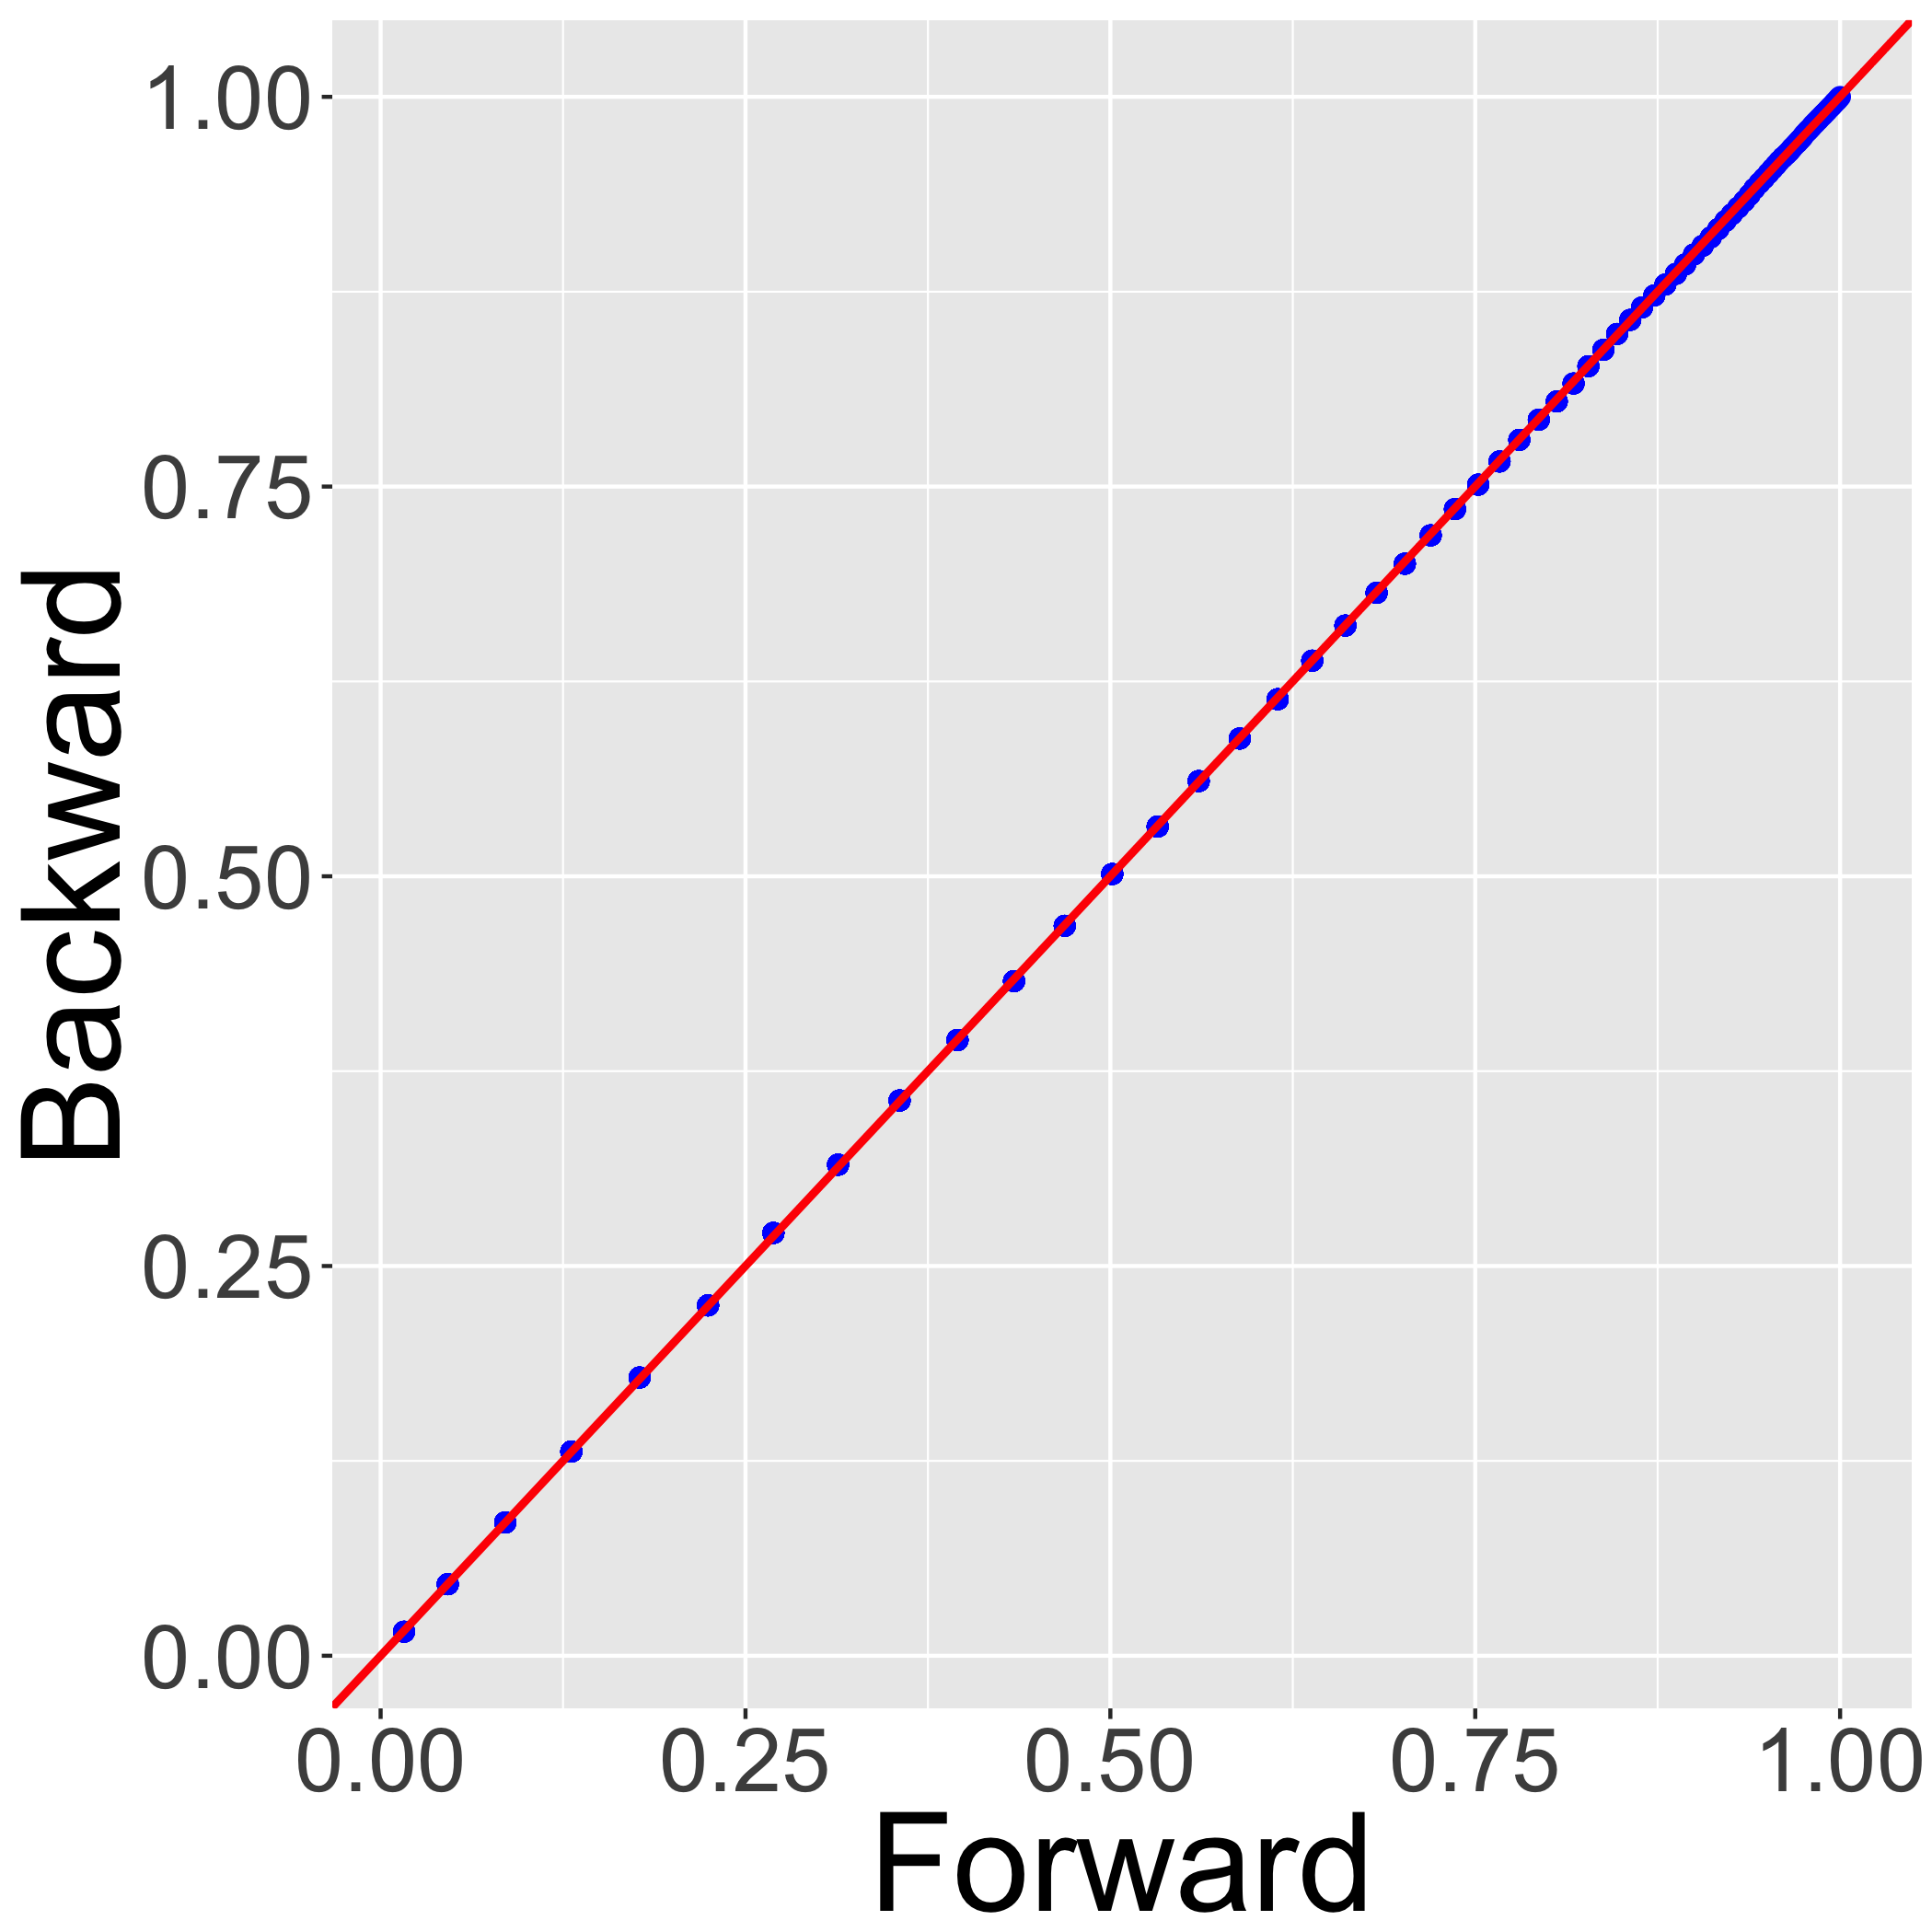
\includegraphics[width=\textwidth]{img/plot1.png}	
   	\end{subfigure}
   	   	\begin{subfigure}[b]{0.2425\textwidth}
   	   		   		   	\caption{Variance of $\lVert \boldsymbol{r}_{d} \rVert_1 $}
   	   		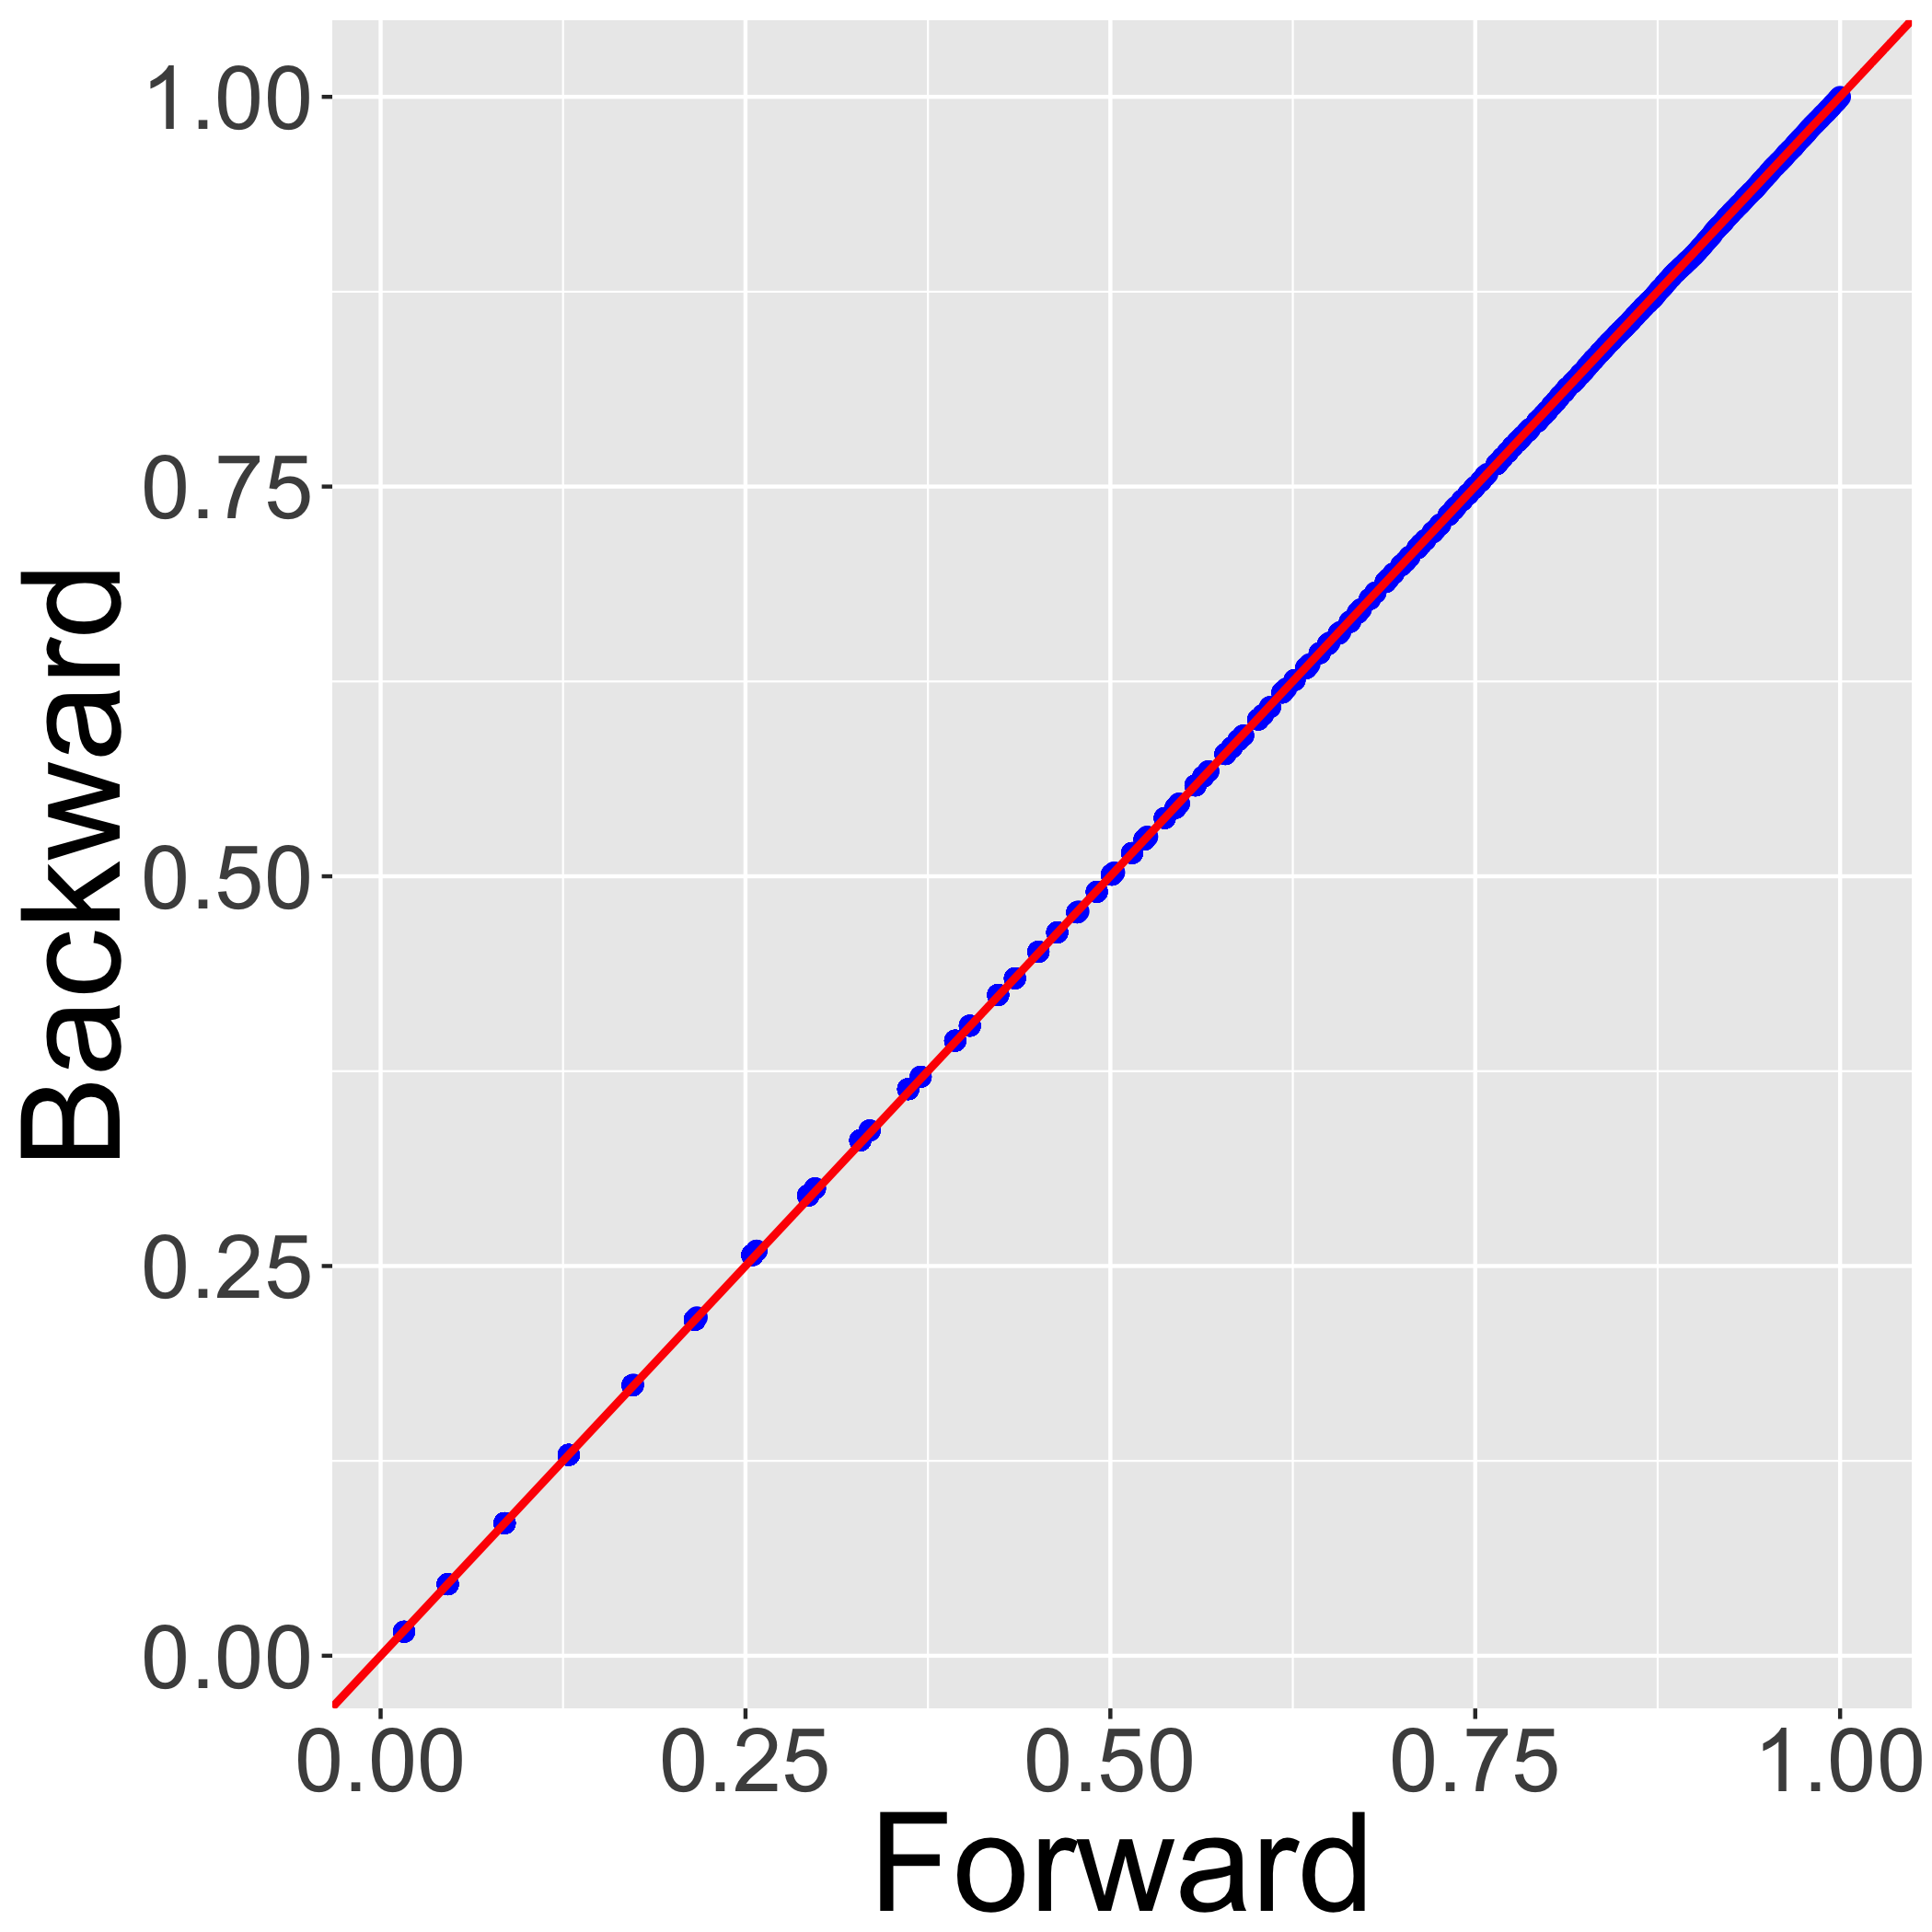
\includegraphics[width=\textwidth]{img/plot2.png}	
   	   	\end{subfigure}
   	   	   	\begin{subfigure}[b]{0.2425\textwidth}
   	   	   		   	   	   		\caption{Mean of $\tau_d$}
   	   	   		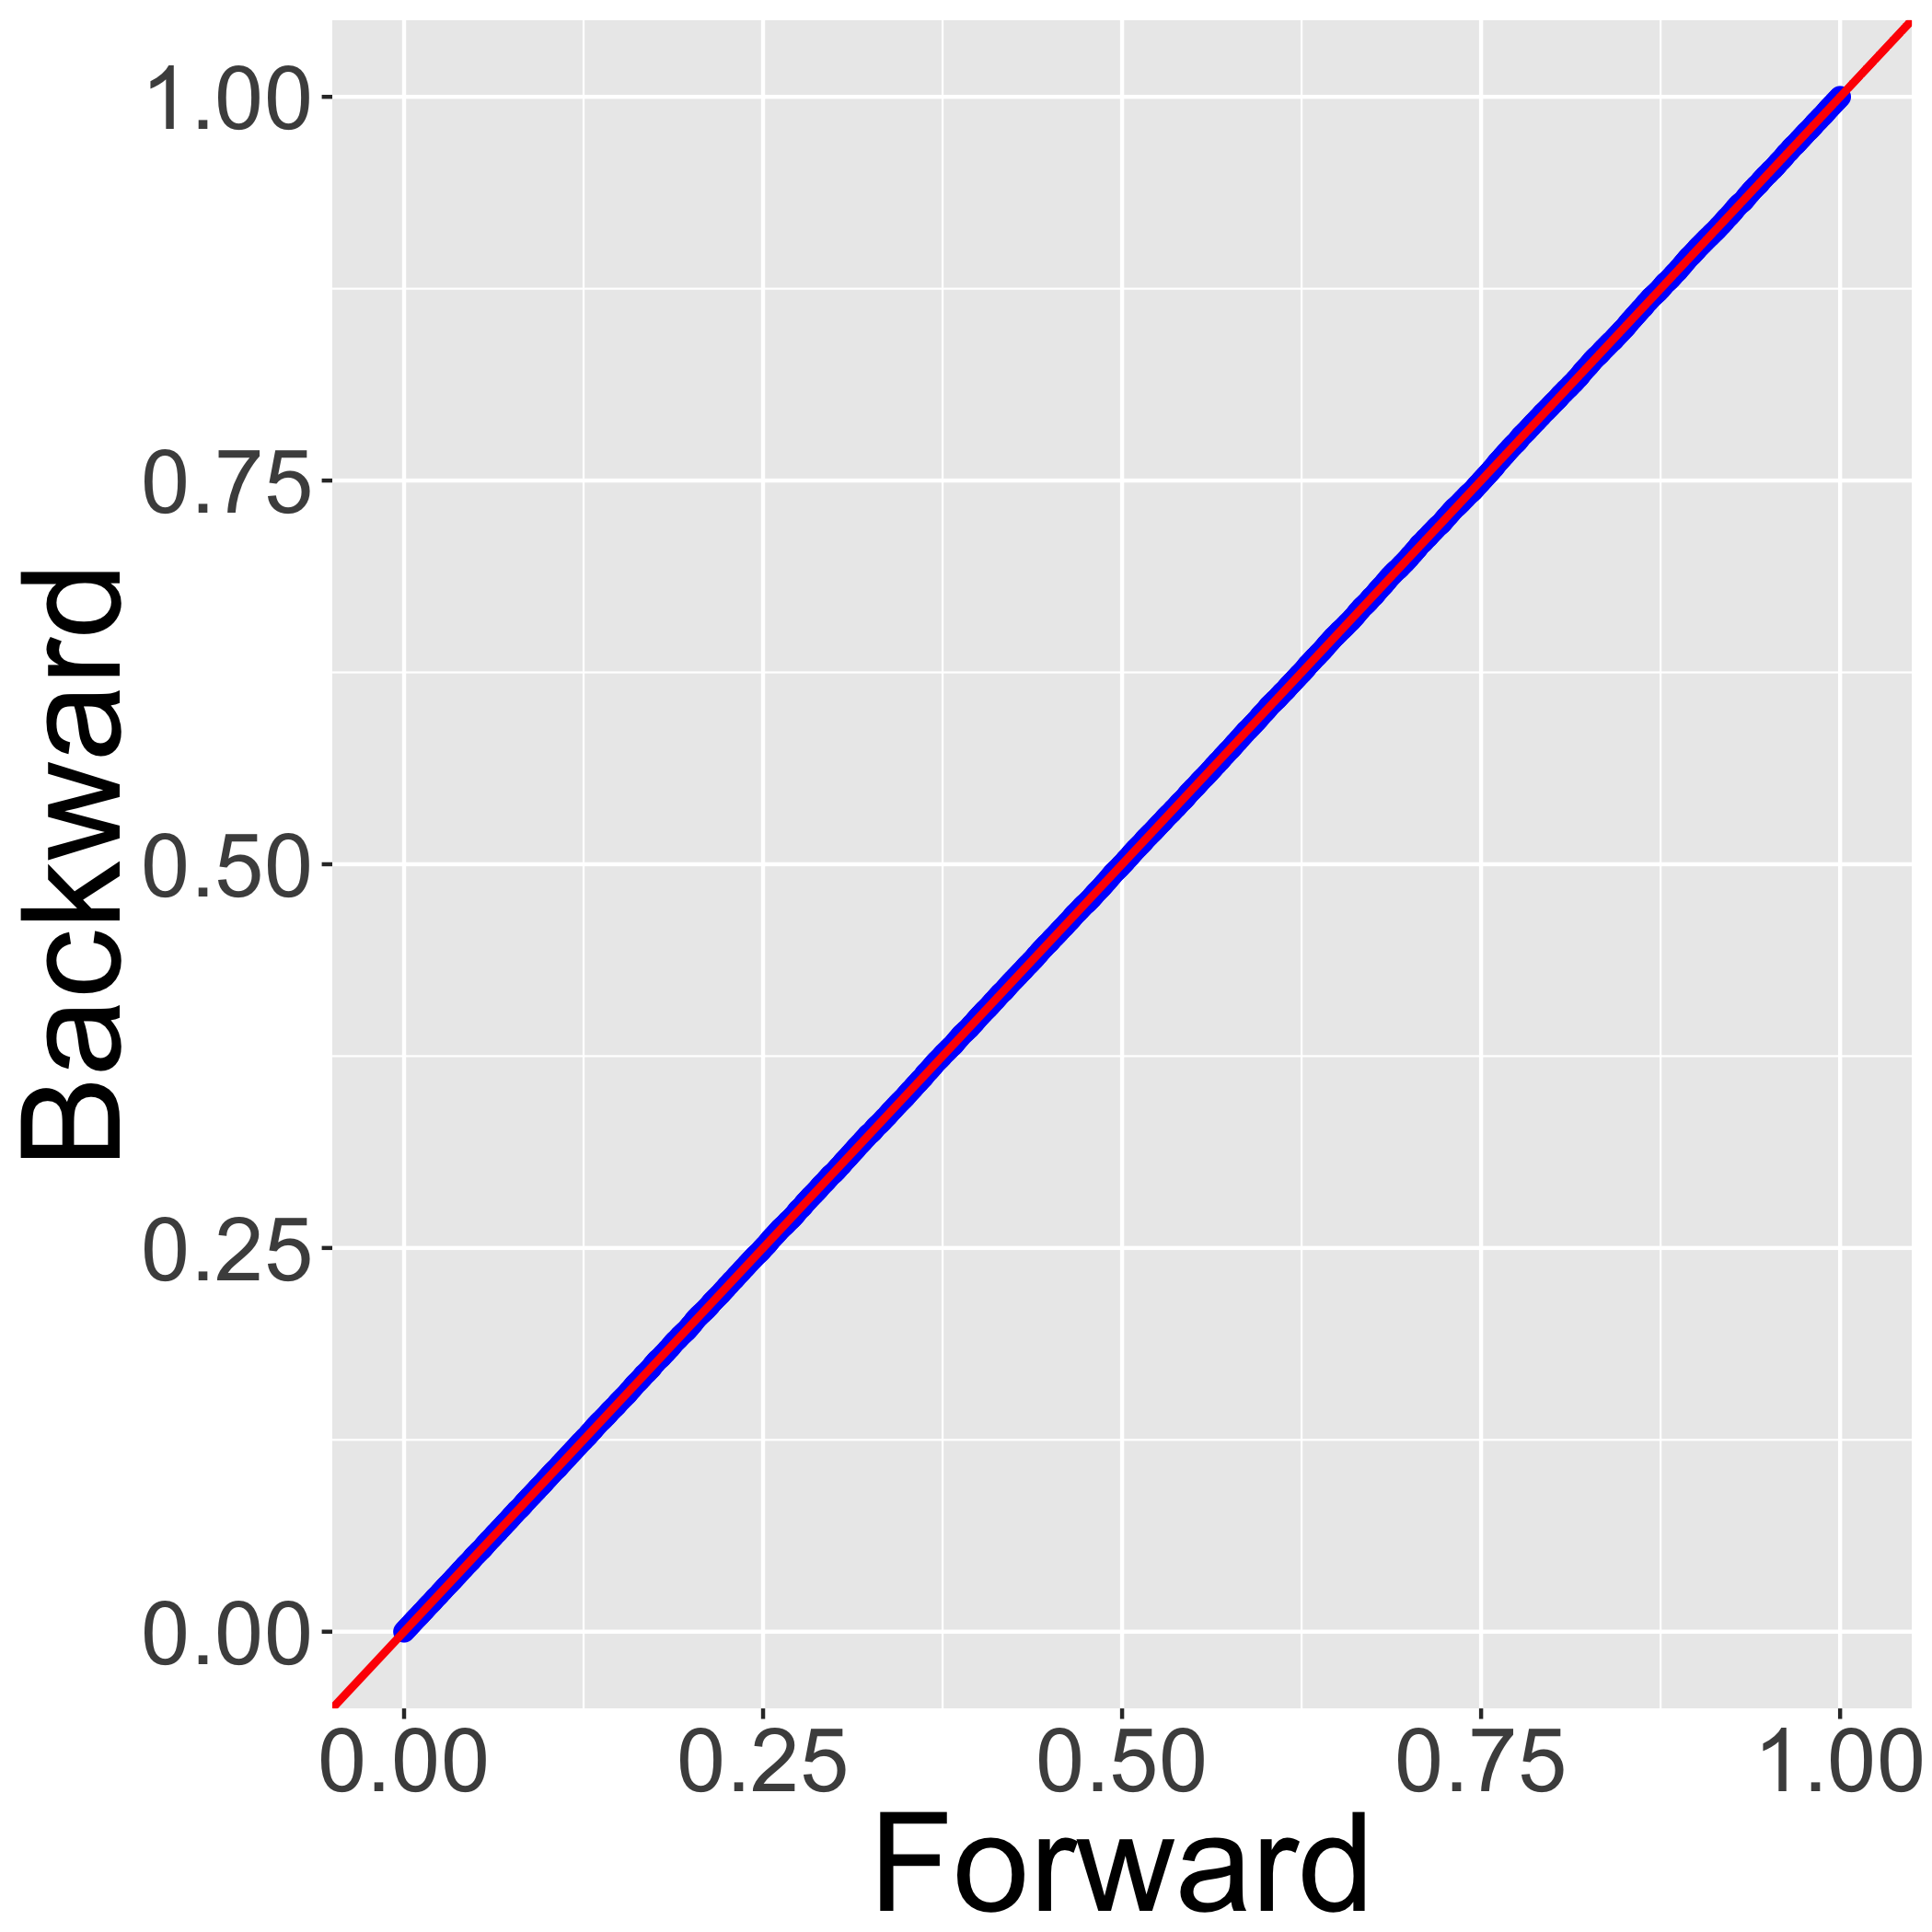
\includegraphics[width=\textwidth]{img/plot3.png}	
   	   	   	\end{subfigure}
   	   	   	   	   	   	\begin{subfigure}[b]{0.2425\textwidth}
   	   	   	   	   	   		  	\caption{Variance of $\tau_d$}
   	   	   	   	   	   		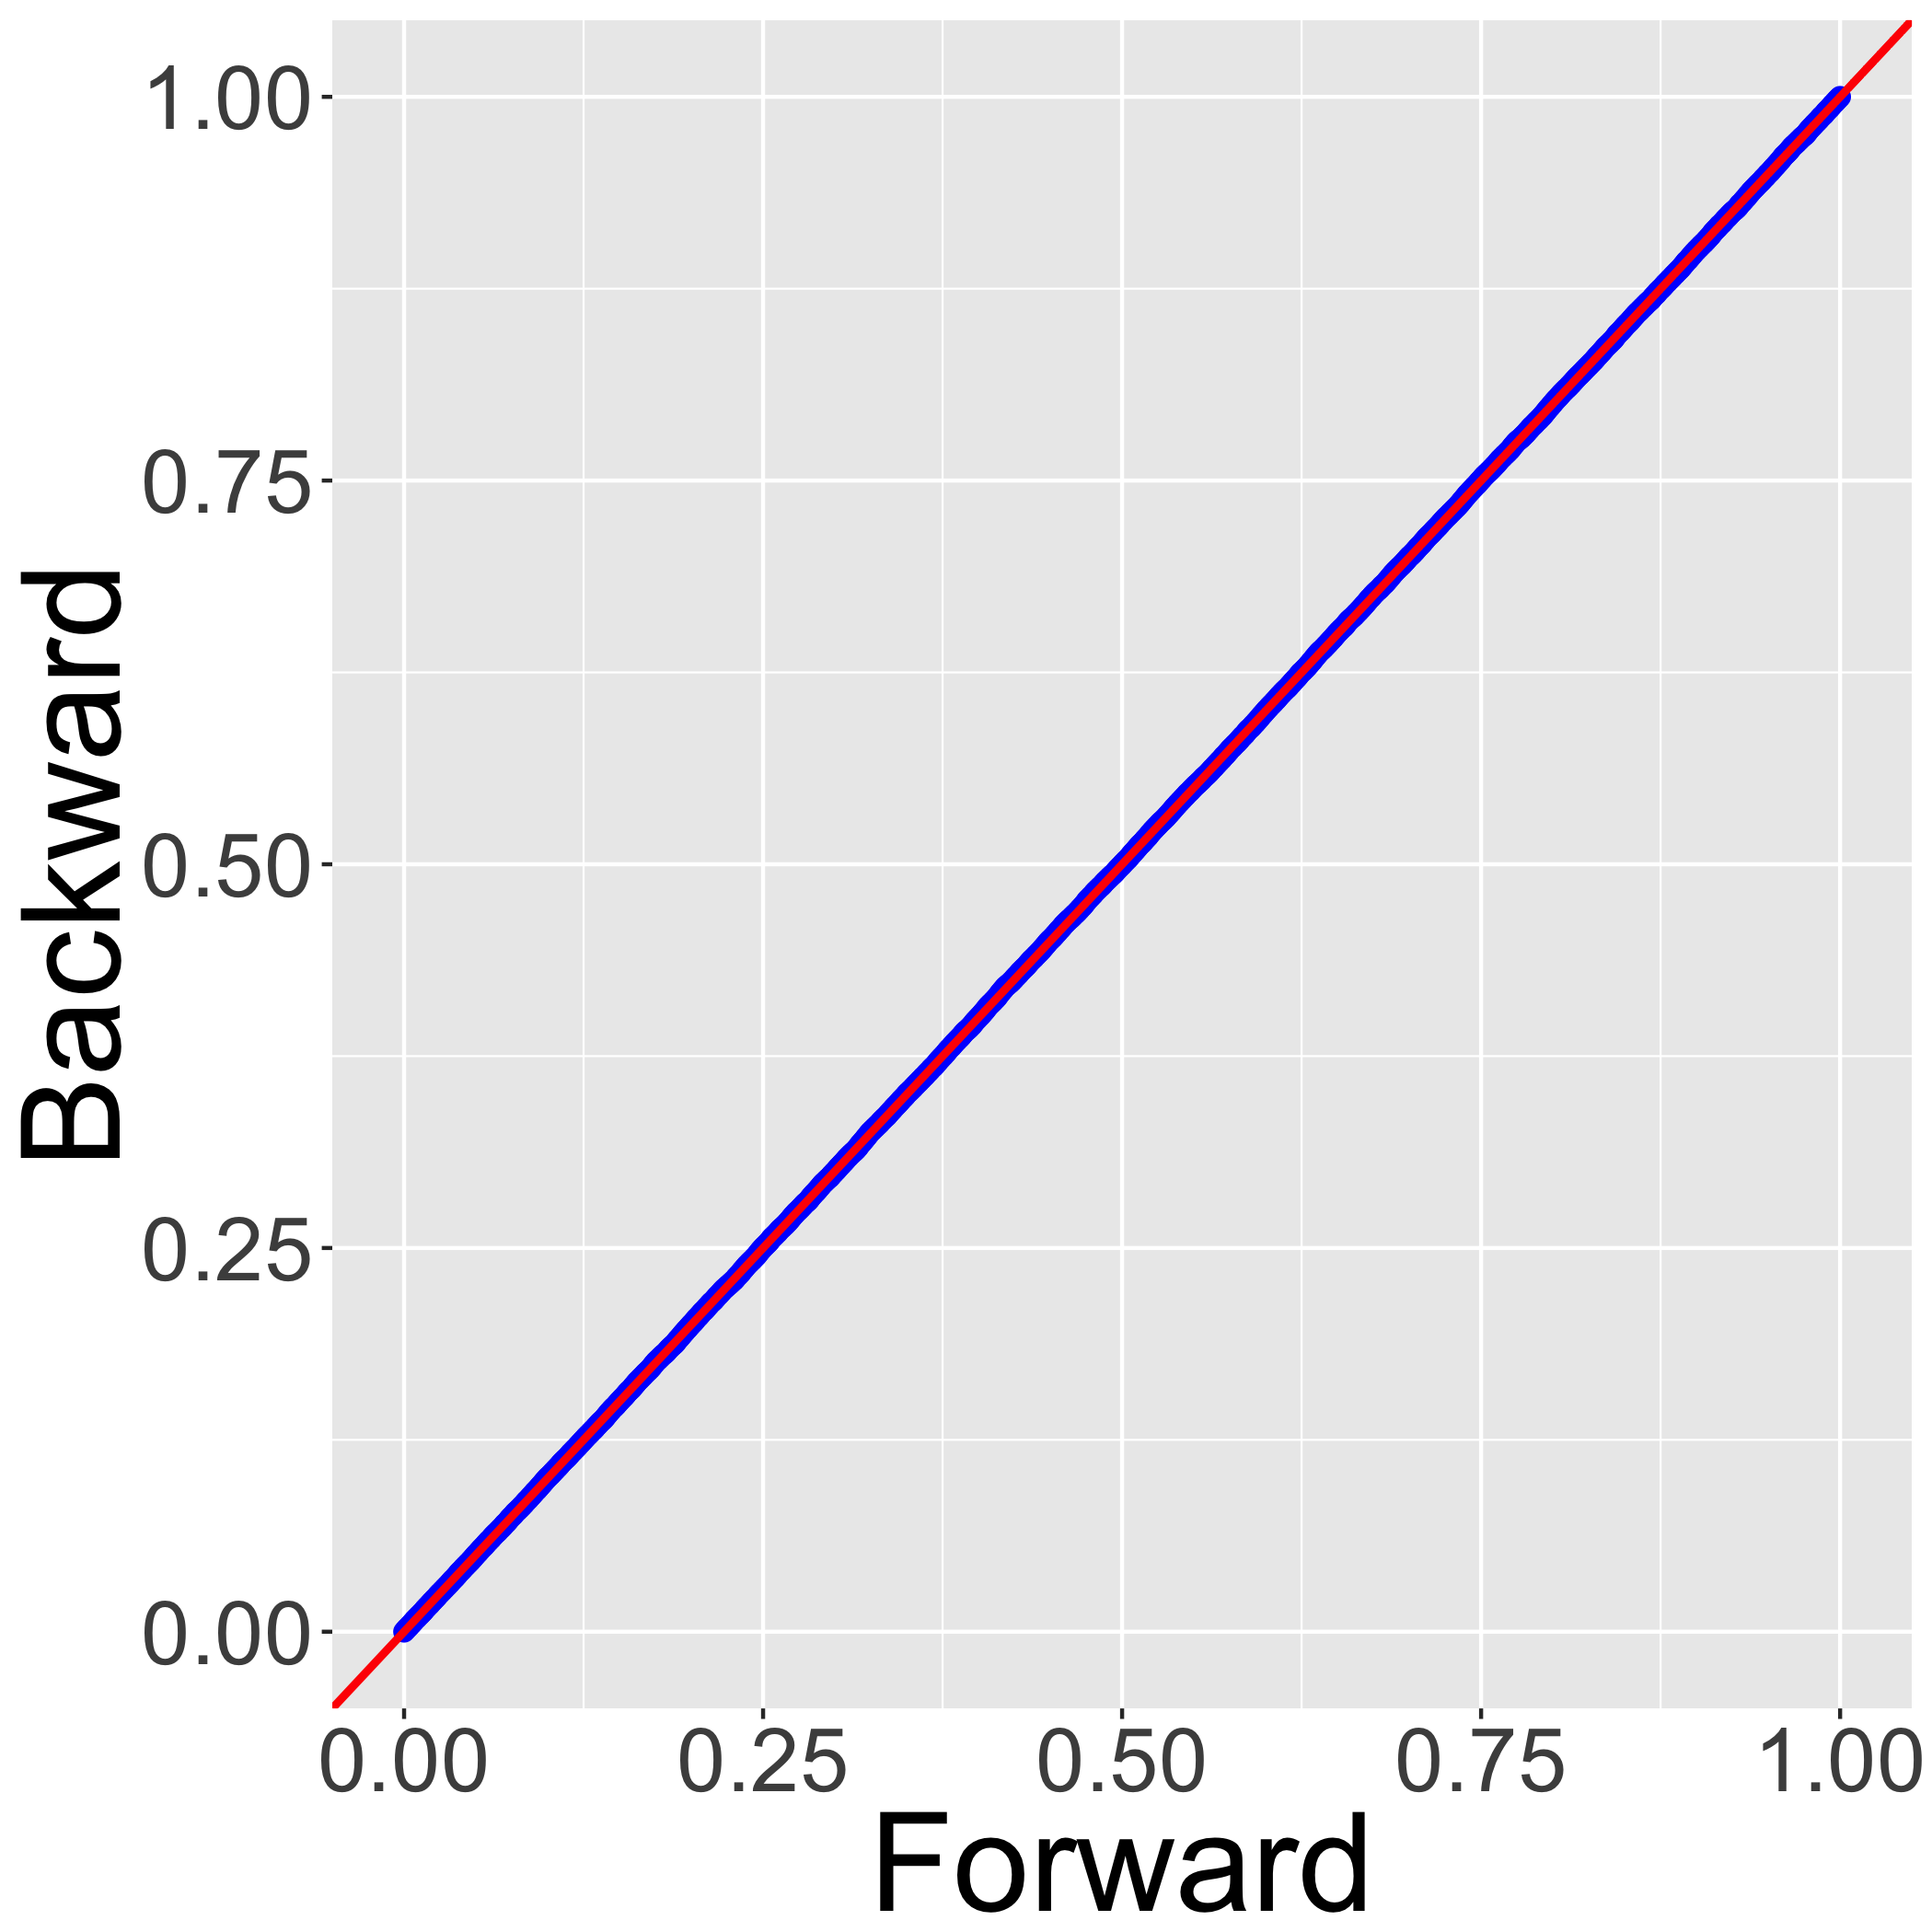
\includegraphics[width=\textwidth]{img/plot4.png}	
   	   	   	   	   	   	\end{subfigure}
   	   	   	   	   	   	   	   	   	   	\begin{subfigure}[b]{0.2425\textwidth}
   	   	   	   	   	   	   	   	   	   		\caption{Value of $b_1$}
   	   	   	   	   	   	   	   	   	   		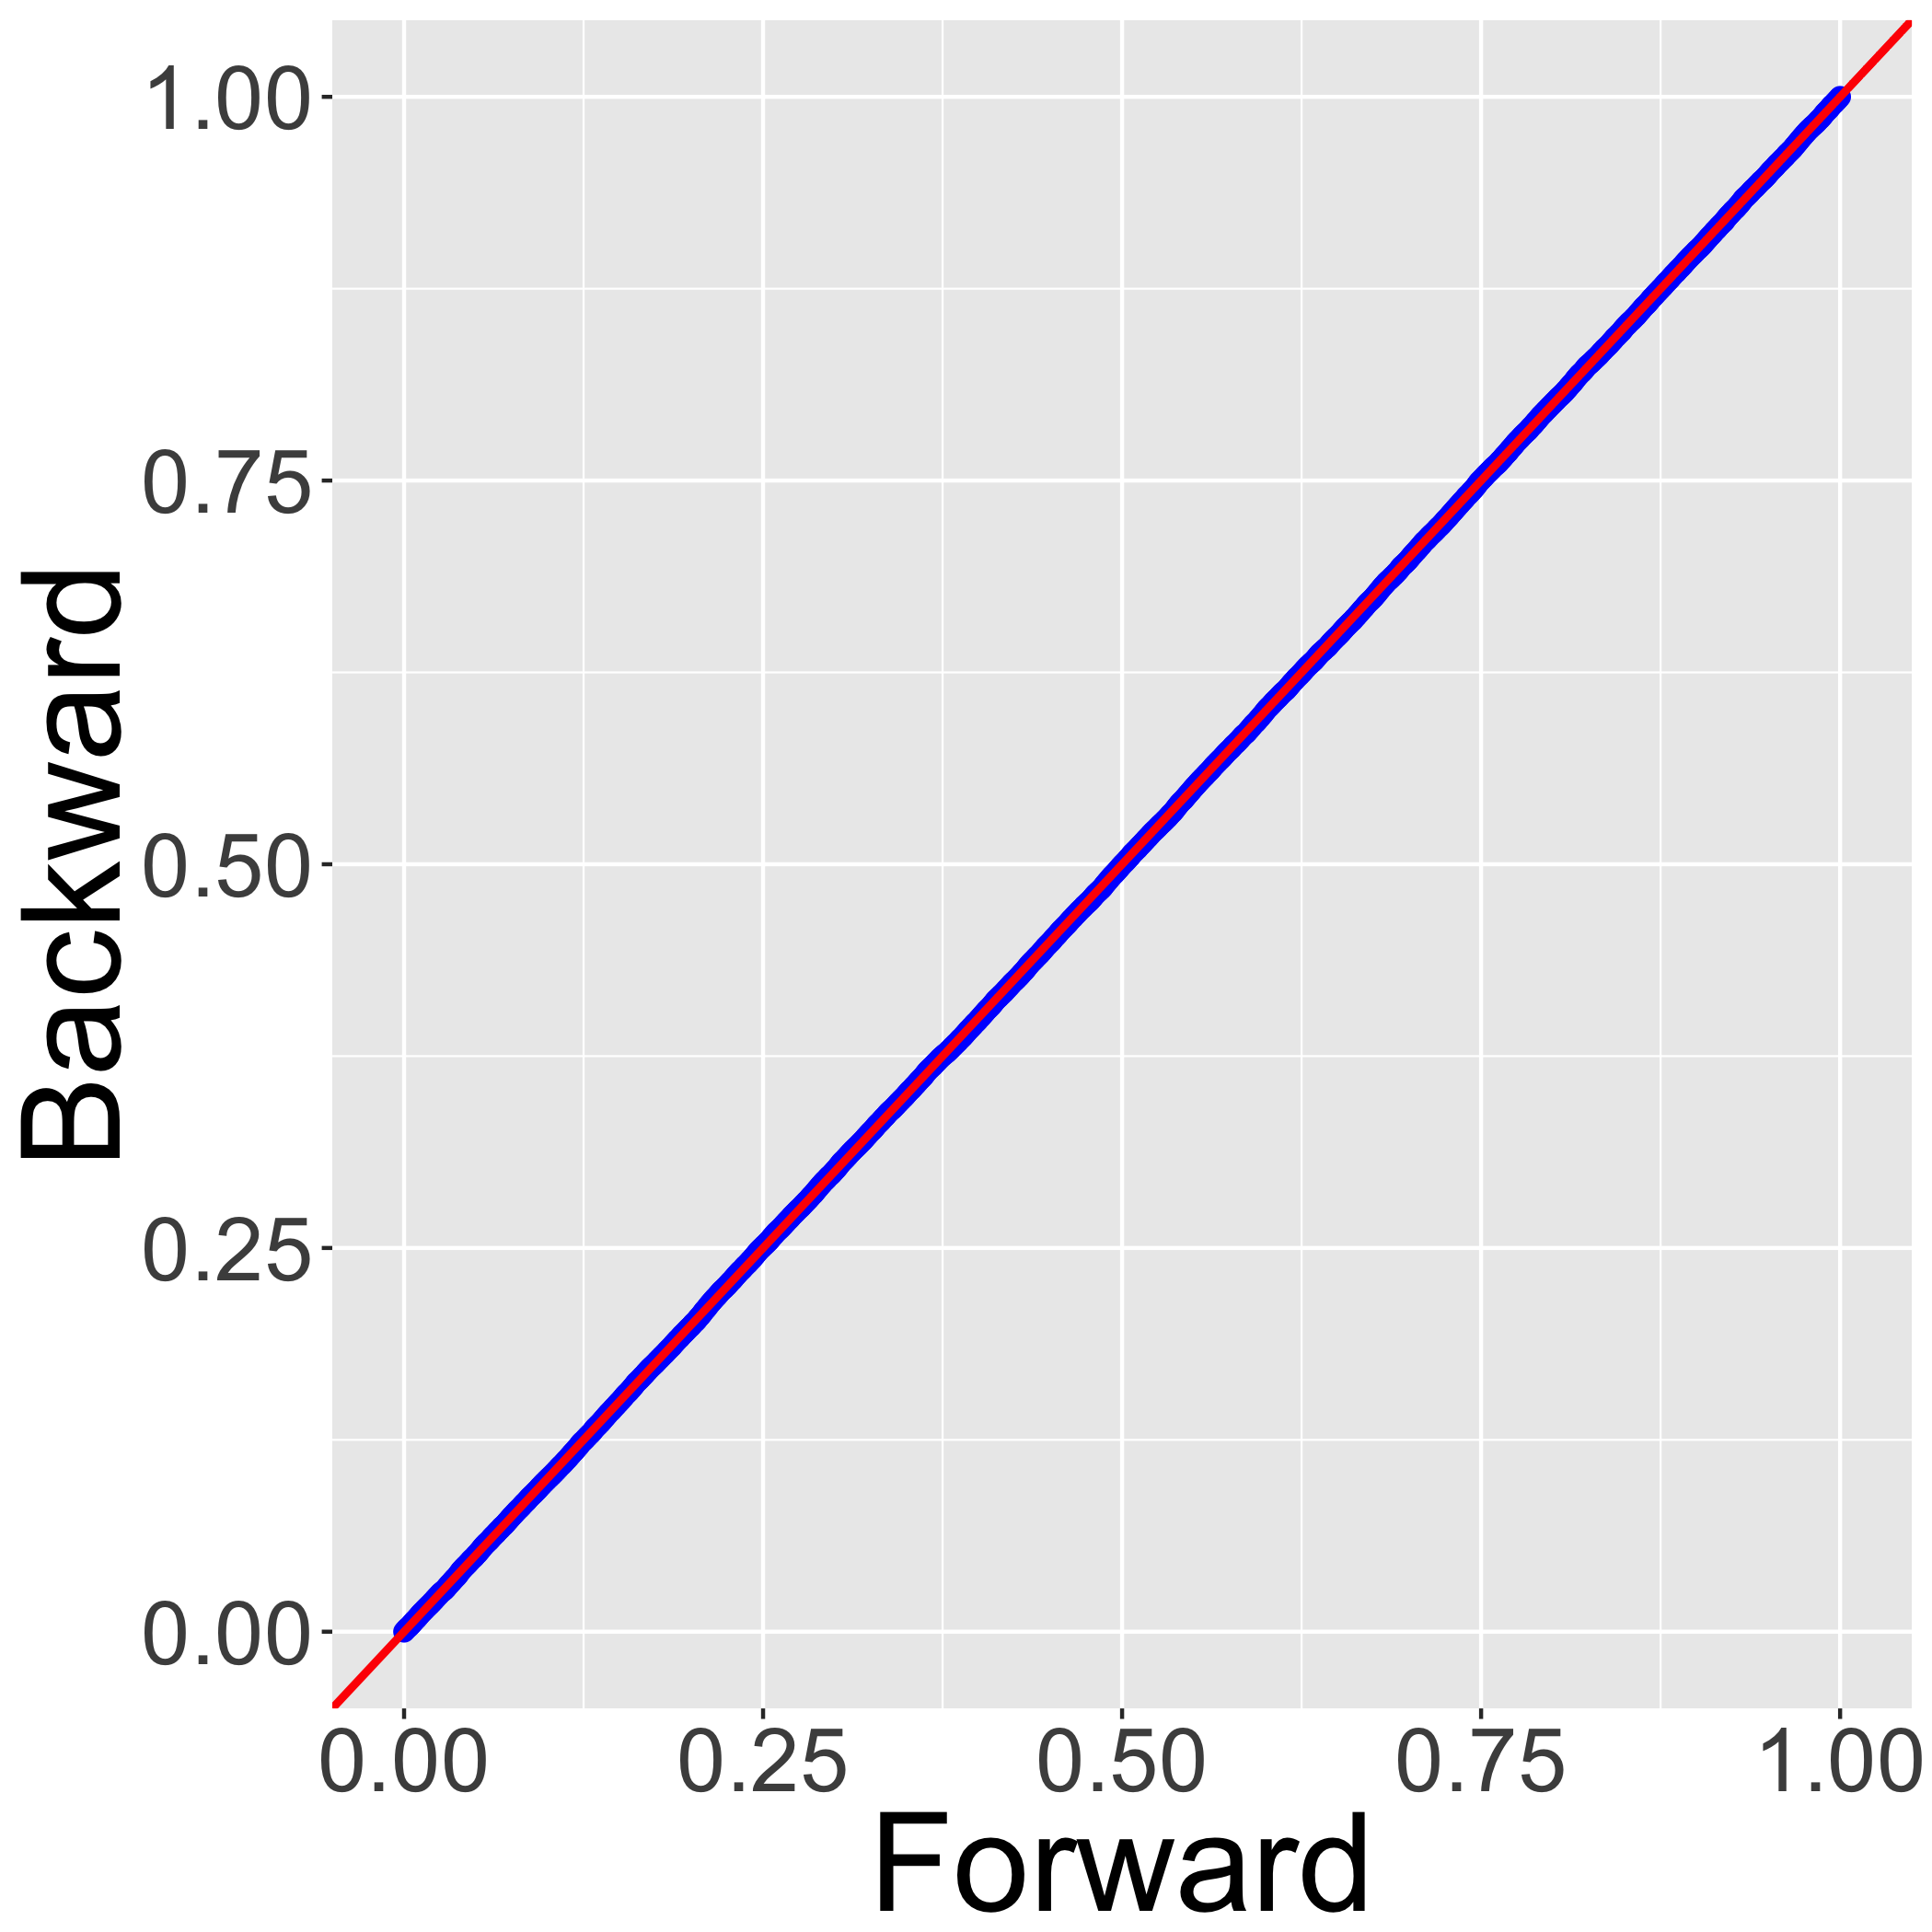
\includegraphics[width=\textwidth]{img/plot5.png}	
   	   	   	   	   	   	   	   	   	   	\end{subfigure}
   	   	   		   	   	\begin{subfigure}[b]{0.2425\textwidth}
   	   	   		   	   		\caption{Value of $b_2$}
   	   	   		   	   		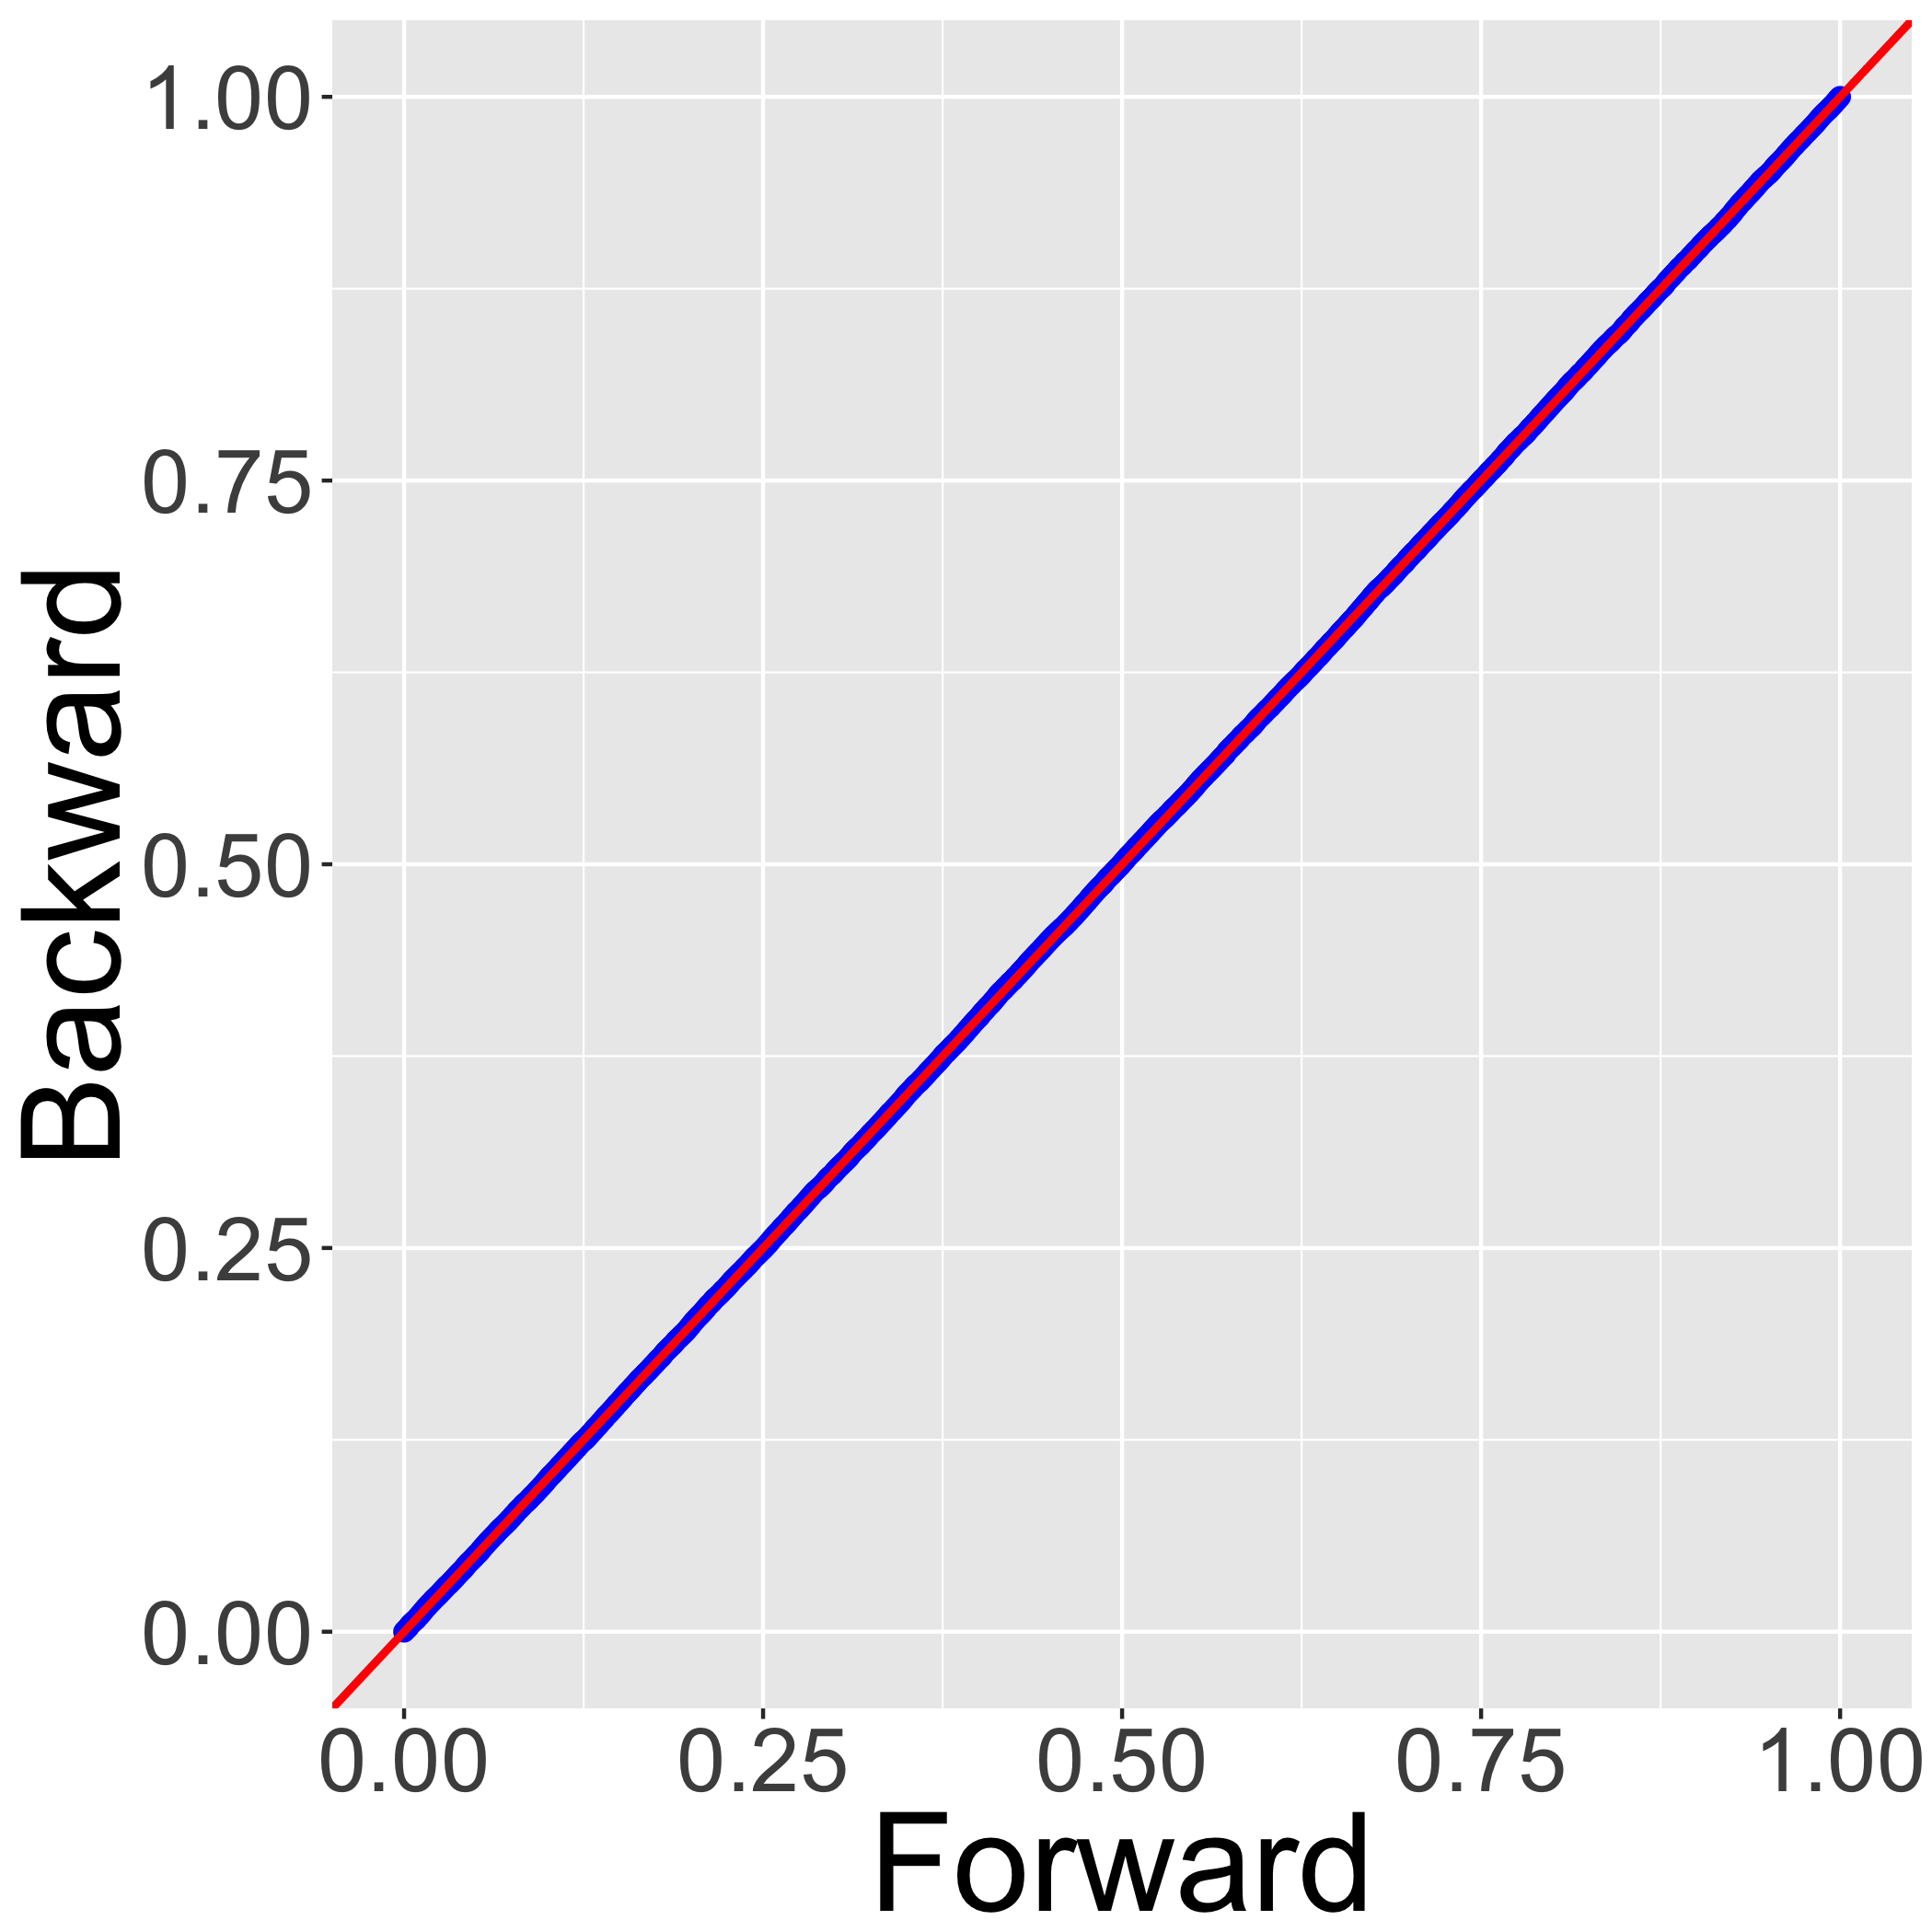
\includegraphics[width=\textwidth]{img/plot6.png}	
   	   	   		   	   	\end{subfigure}   	   	   	   	   	   	   	
   		   	   	\begin{subfigure}[b]{0.2425\textwidth}
   		   	   		\caption{Value of $b_3$}
   		   	   		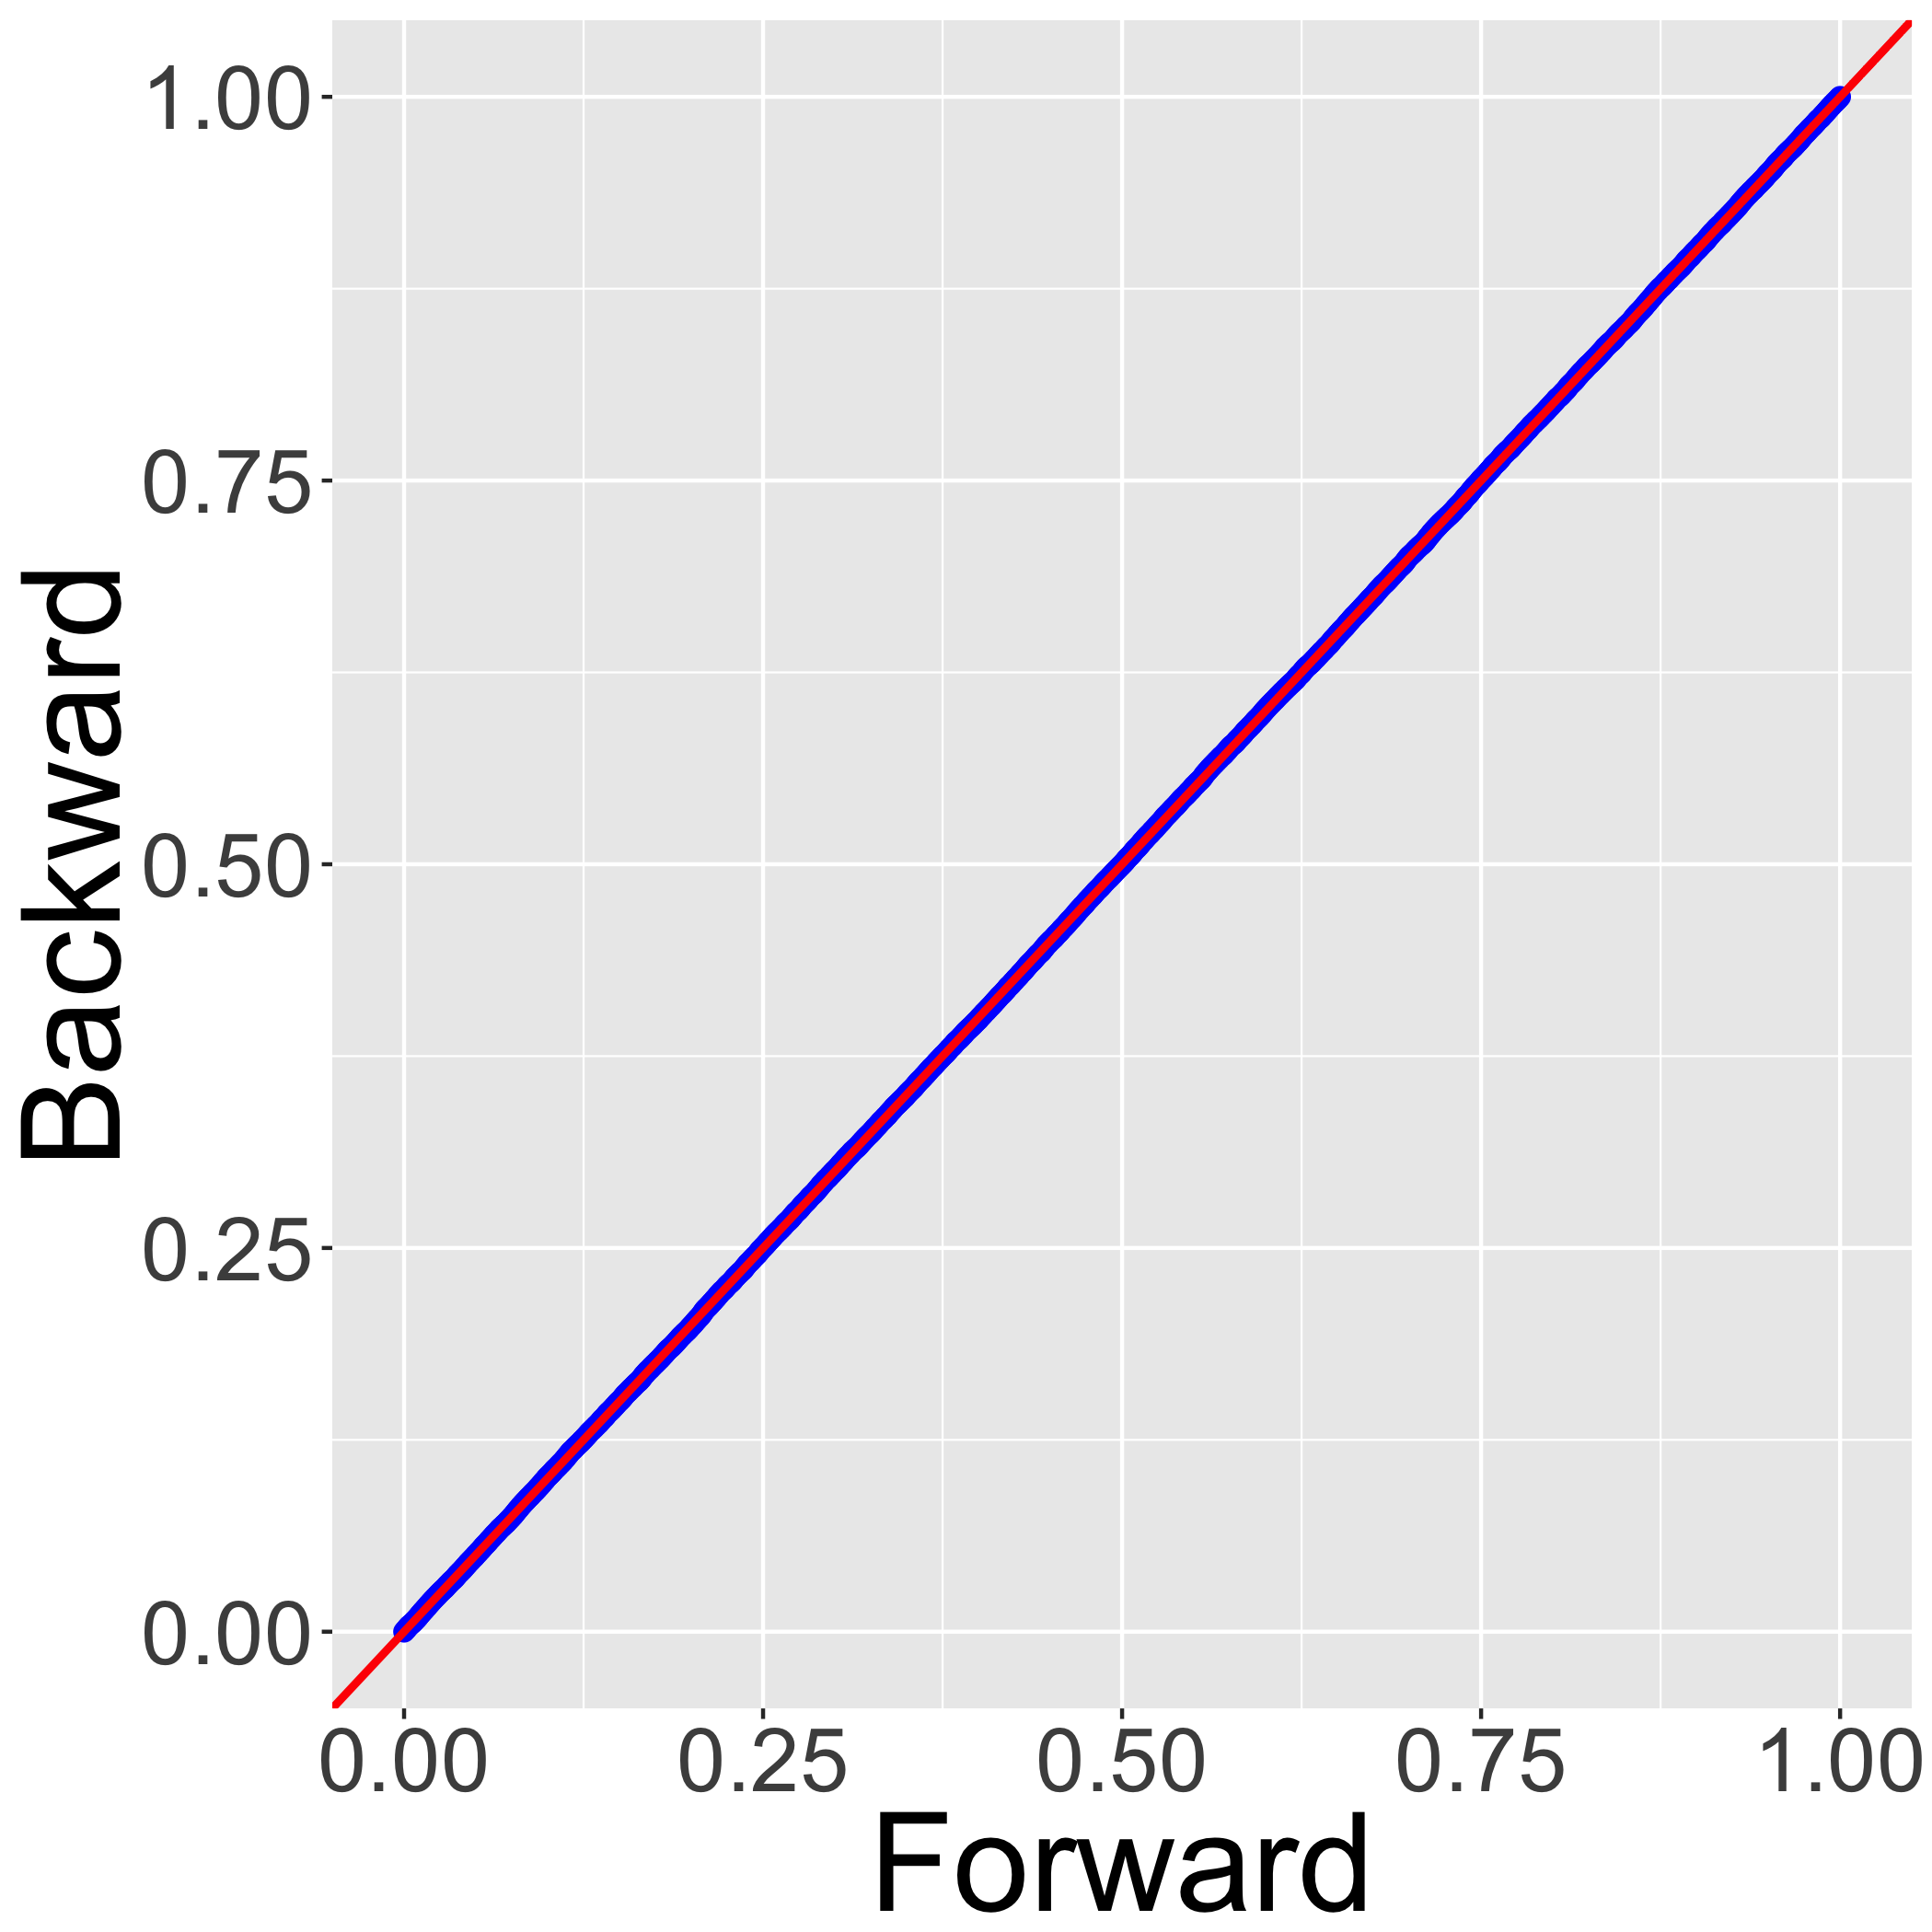
\includegraphics[width=\textwidth]{img/plot7.png}	
   		   	   	\end{subfigure}   	   		   	   	
   		   	   	   		   	   	\begin{subfigure}[b]{0.2425\textwidth}
   		   	   	   		   	   		\caption{Value of $b_4$}
   		   	   	   		   	   		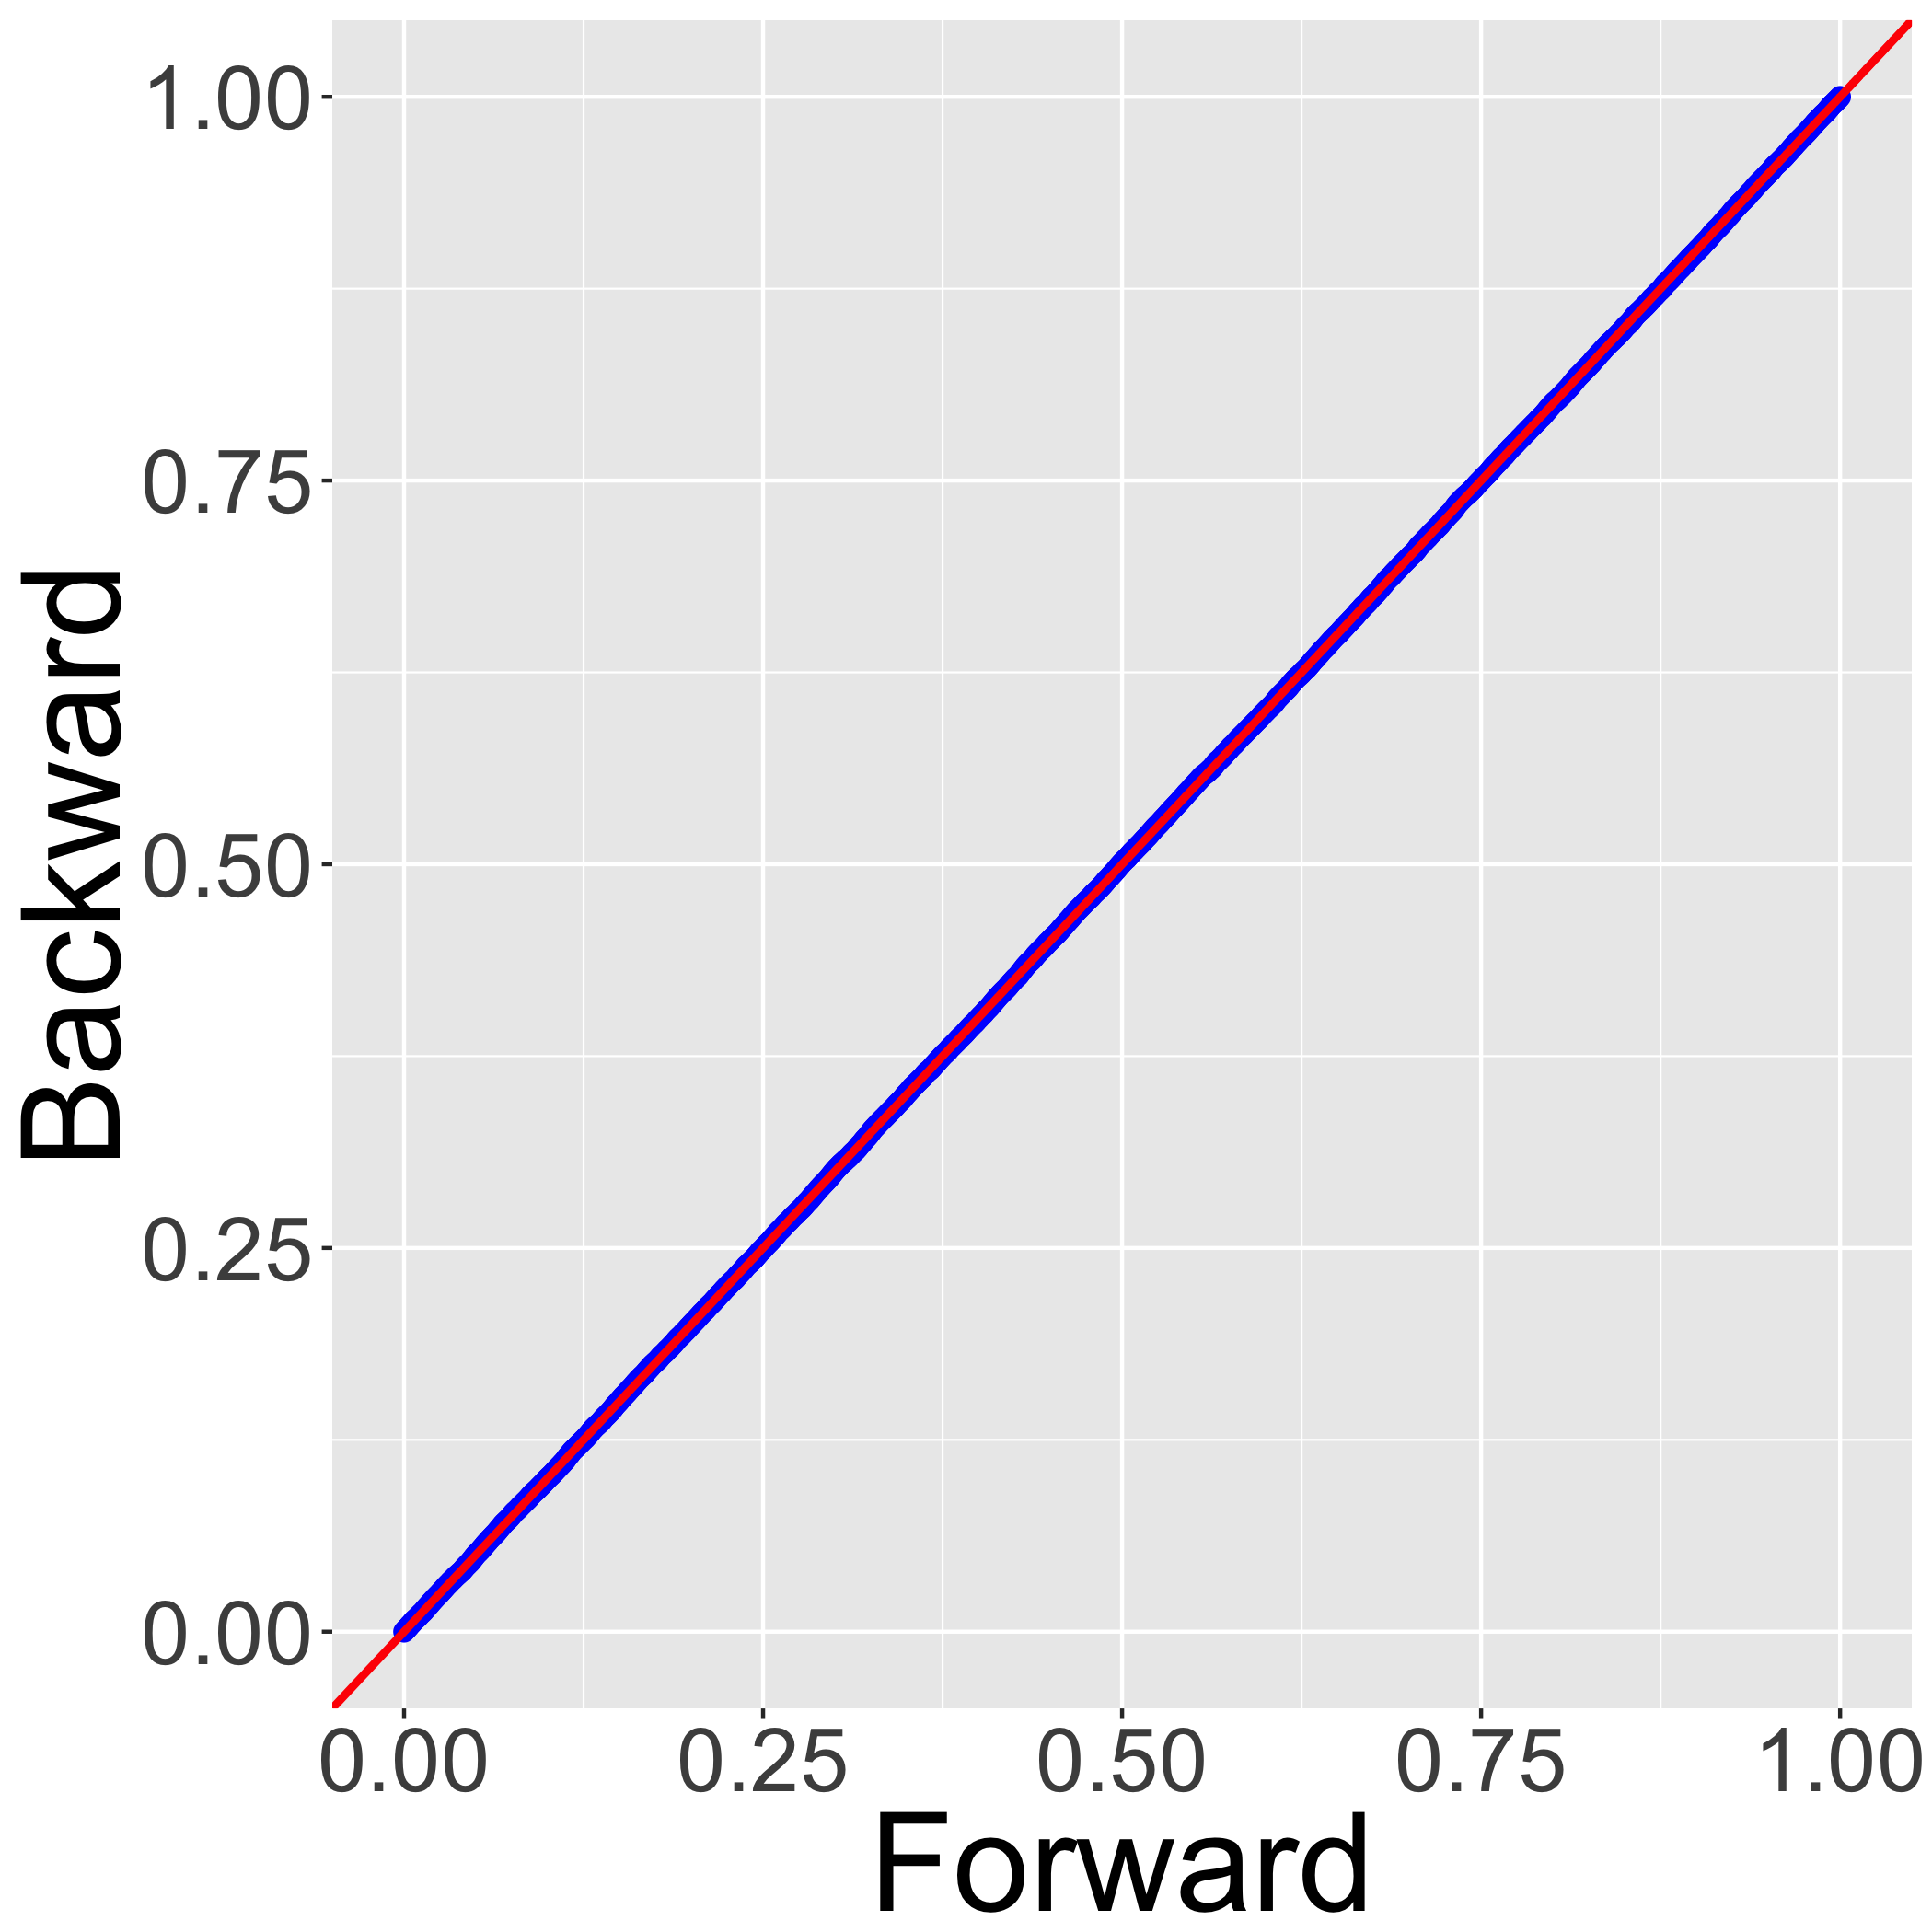
\includegraphics[width=\textwidth]{img/plot8.png}	
   		   	   	   		   	   	\end{subfigure}   	   		   	   	
   		   	   	   		   	   	   		   	   	\begin{subfigure}[b]{0.2425\textwidth}
   		   	   	   		   	   	   		   	   		\caption{Value of $\eta_1$}
   		   	   	   		   	   	   		   	   		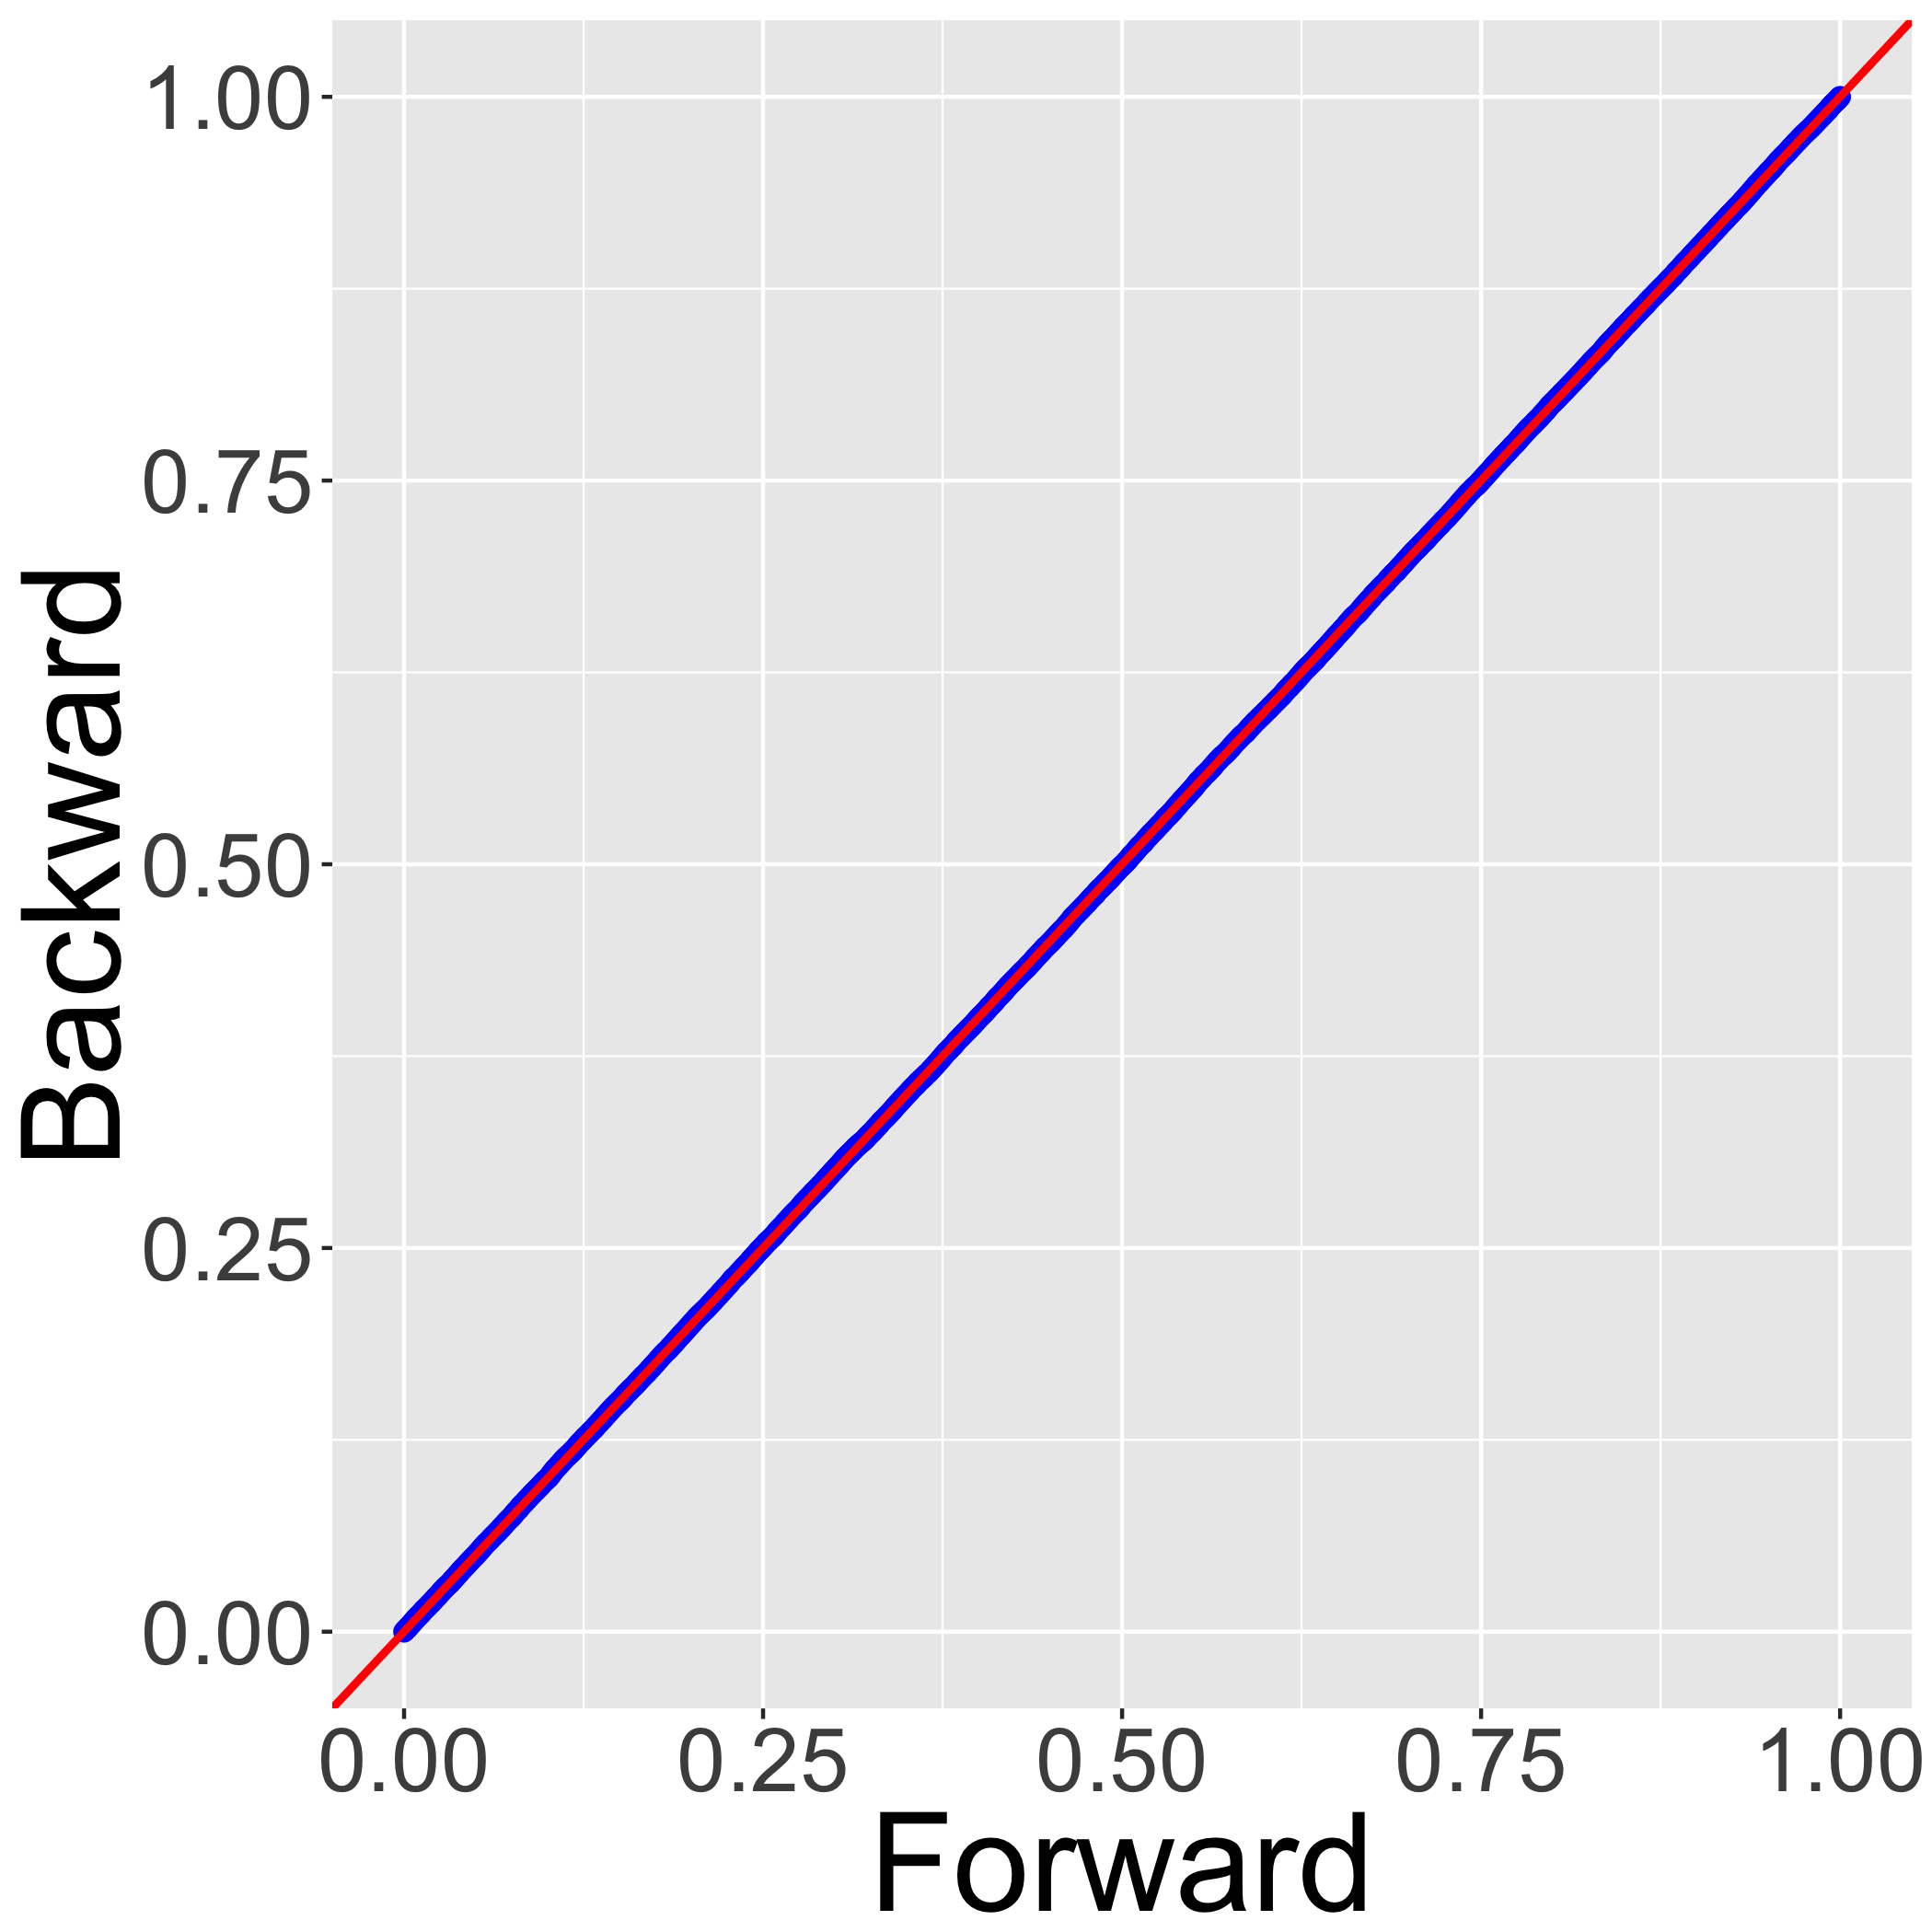
\includegraphics[width=\textwidth]{img/plot9.png}	
   		   	   	   		   	   	   		   	   	\end{subfigure}   	   		   	   	
   		     		   	   	\begin{subfigure}[b]{0.2425\textwidth}
   		     		   	   		\caption{Value of $\eta_2$}
   		     		   	   		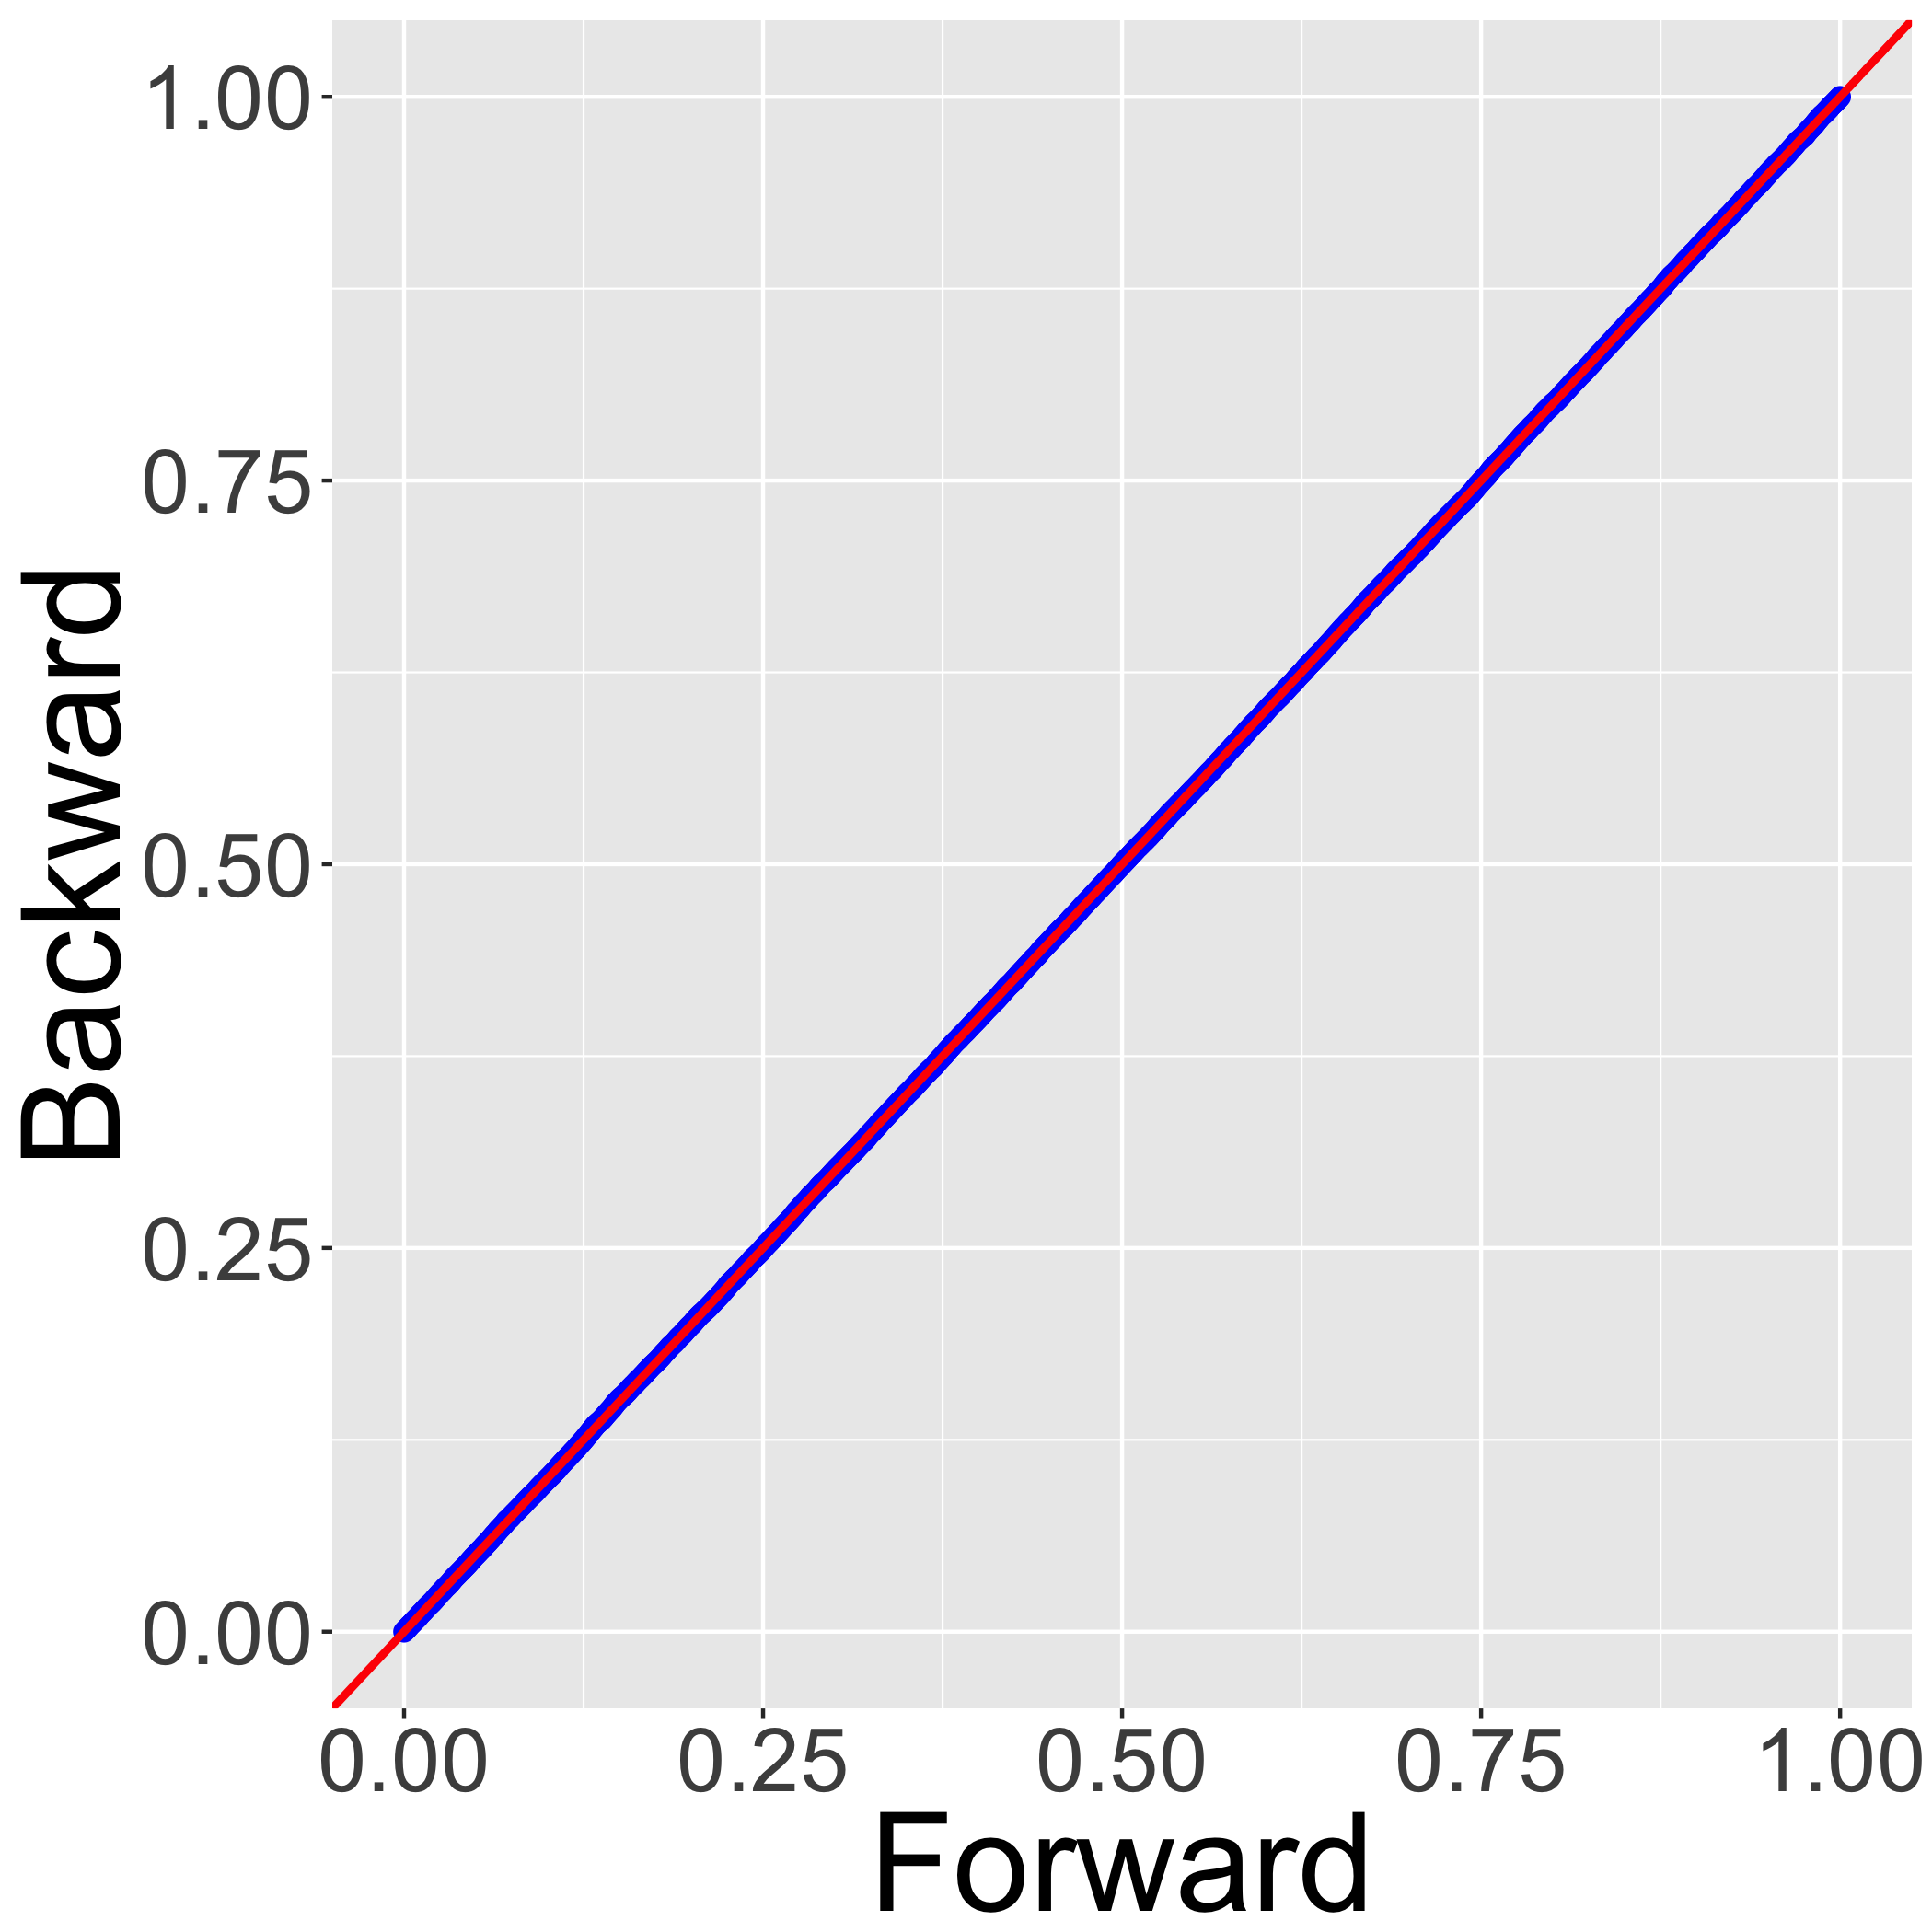
\includegraphics[width=\textwidth]{img/plot10.png}	
   		     		   	   	\end{subfigure}   	   		   	   	
   		   	     		   	   	\begin{subfigure}[b]{0.2425\textwidth}
   		   	     		   	   		\caption{Value of $\eta_3$}
   		   	     		   	   		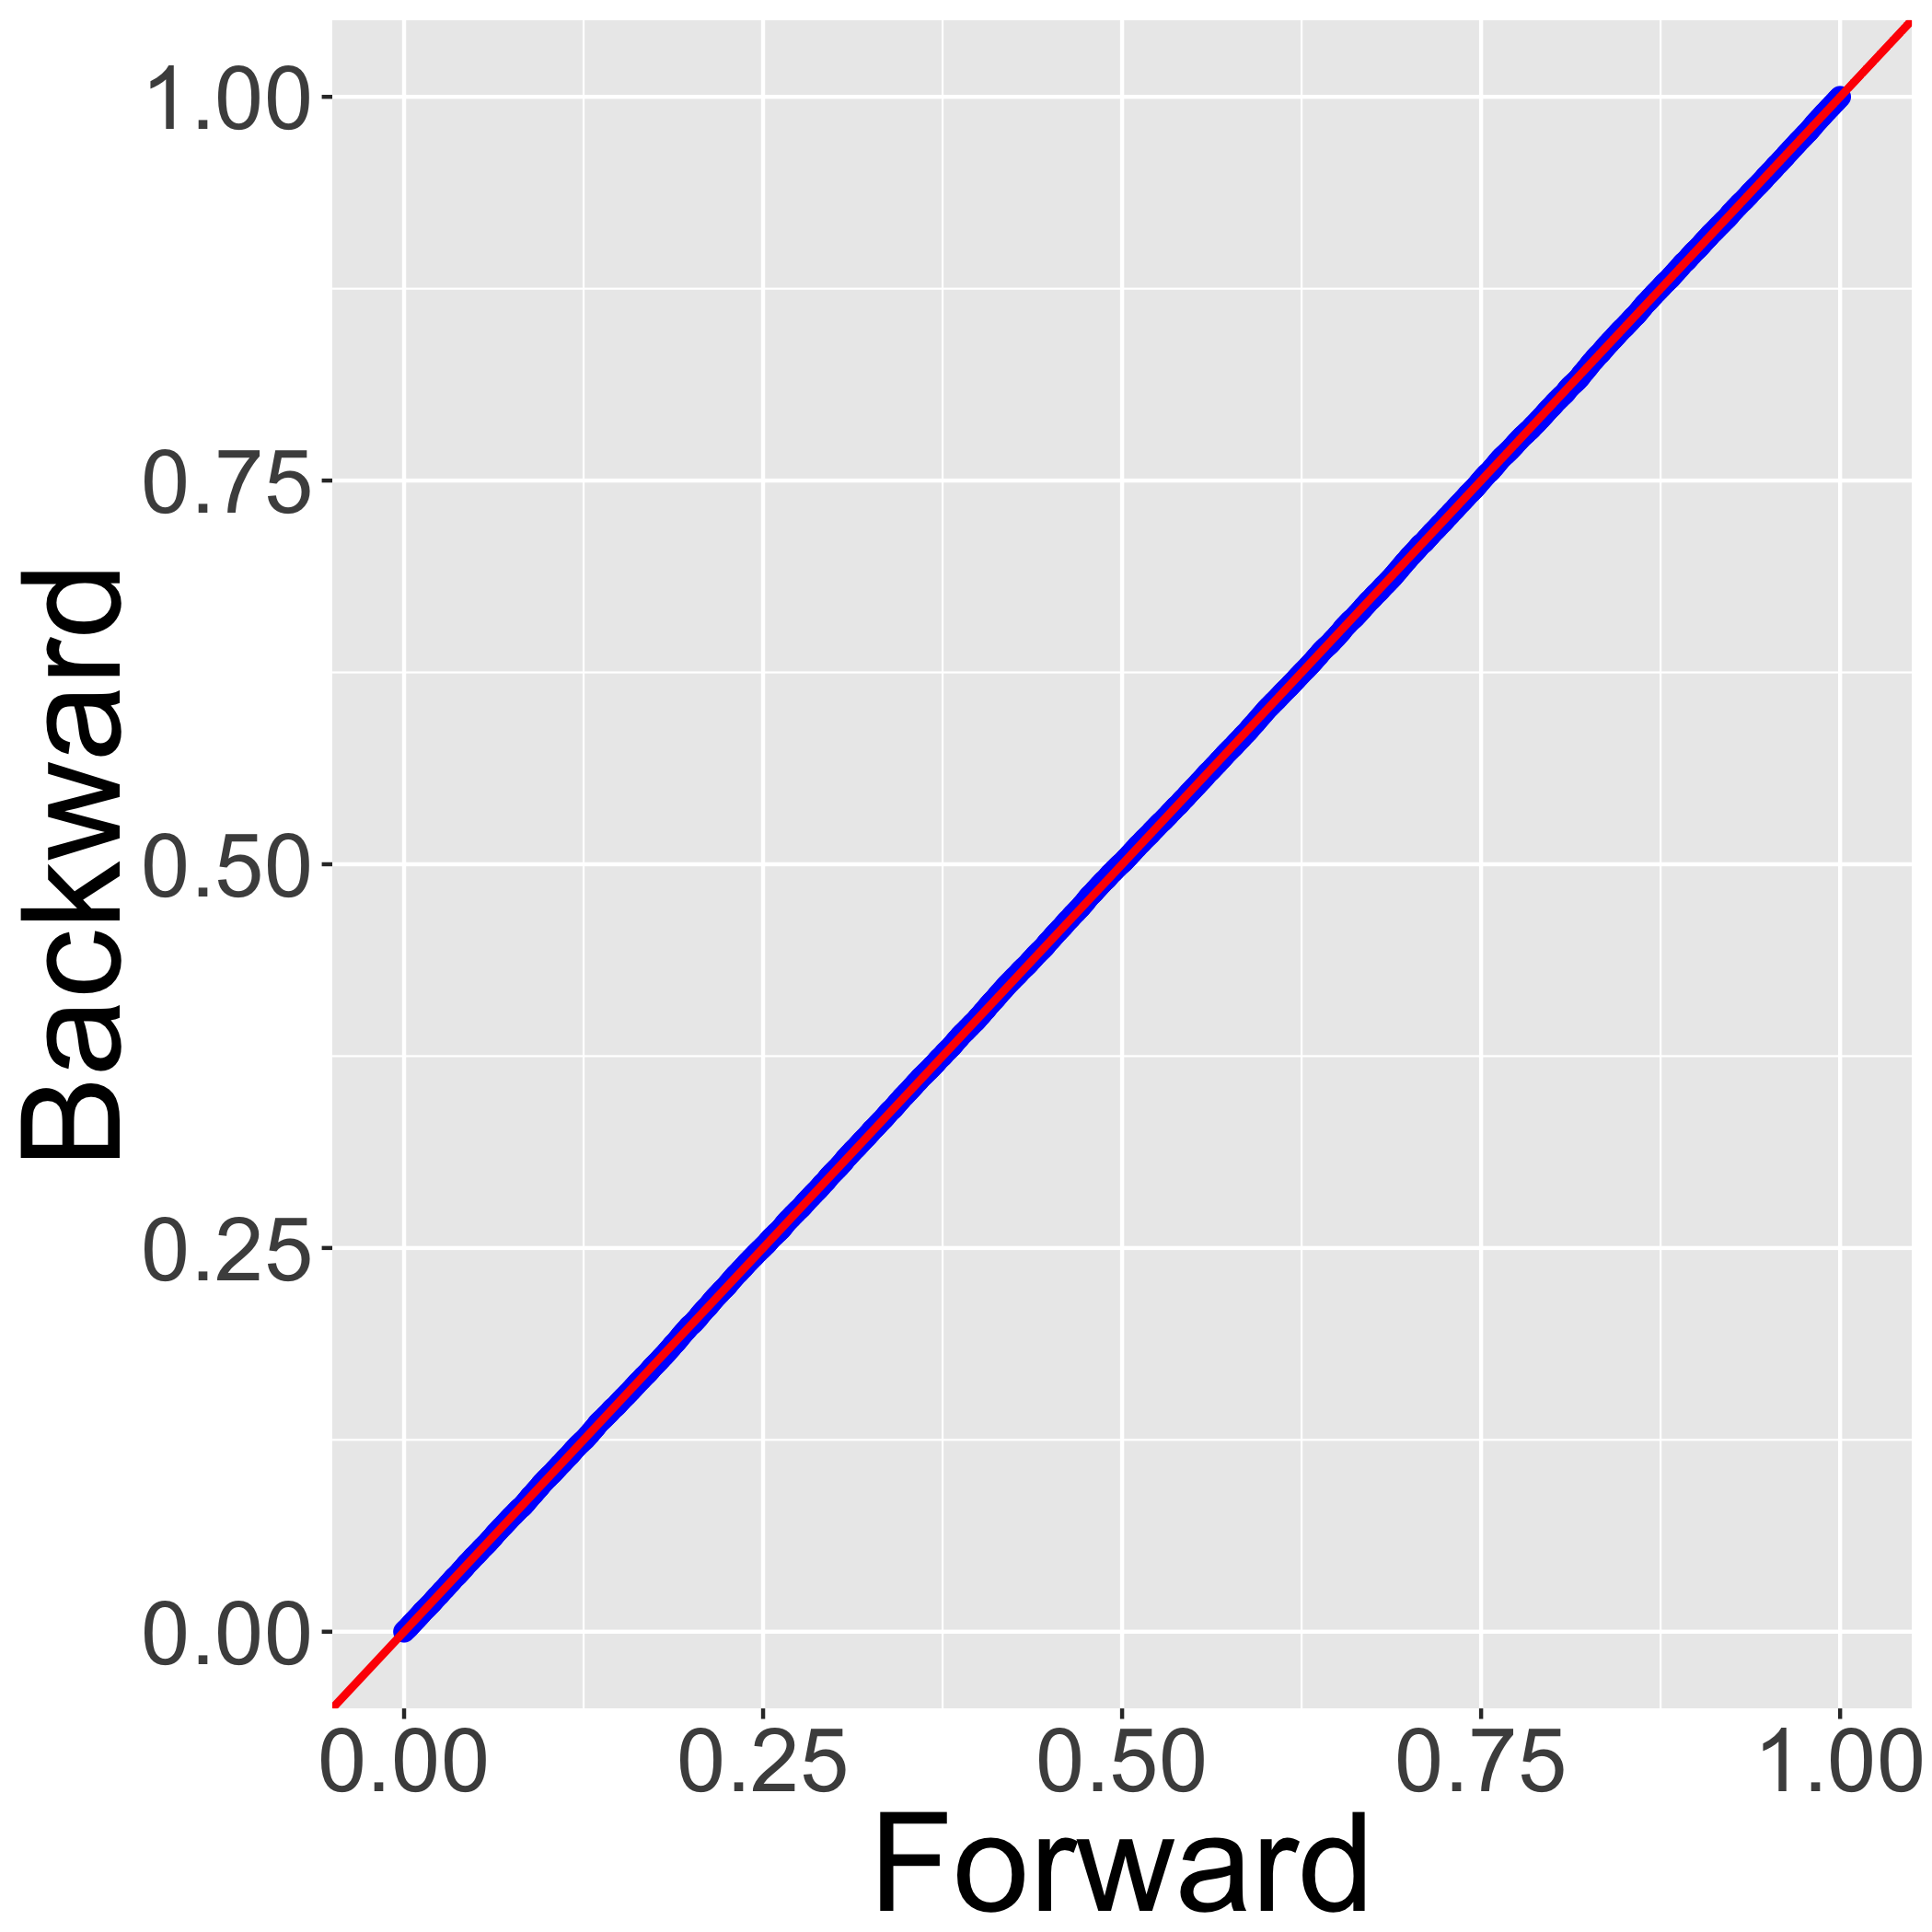
\includegraphics[width=\textwidth]{img/plot11.png}	
   		   	     		   	   	\end{subfigure}   	   		   	   	  		   	   	 	
   		   	     		   	   		     		   	   	\begin{subfigure}[b]{0.2425\textwidth}
   		   	     		   	   		     		   	   		\caption{Value of $\sigma^2_\tau$}
   		   	     		   	   		     		   	   		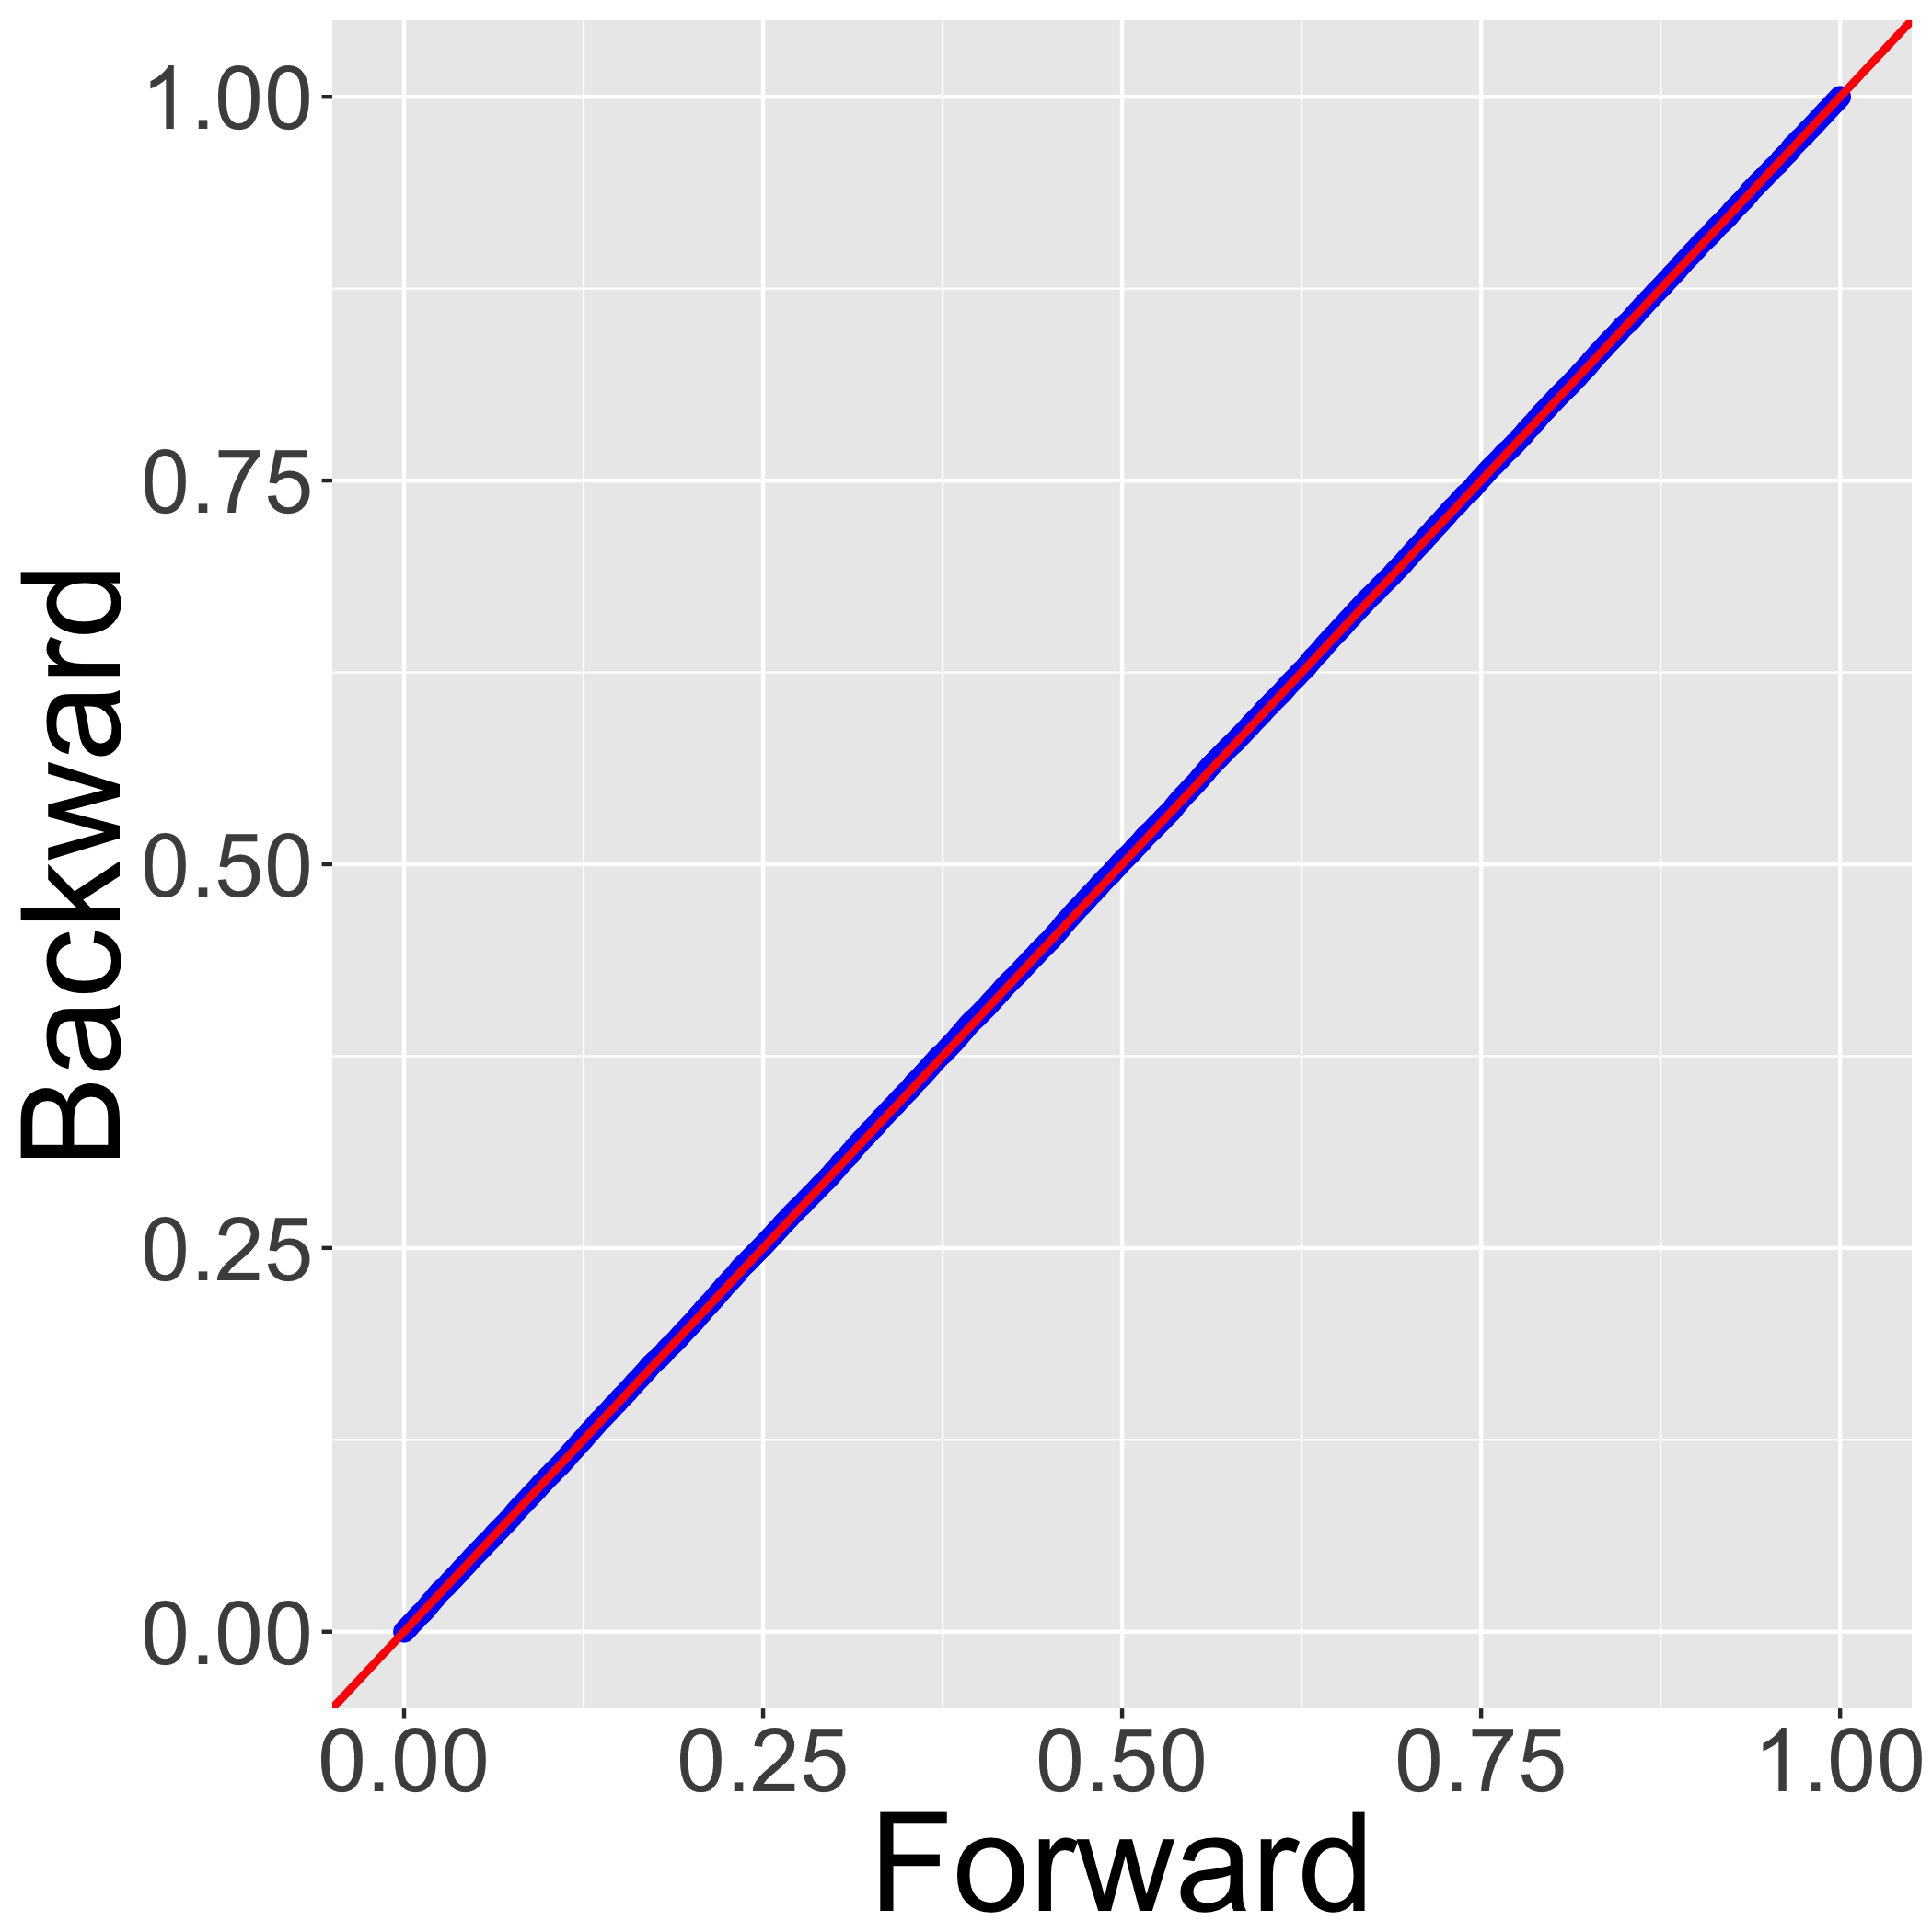
\includegraphics[width=\textwidth]{img/plot12.png}	
   		   	     		   	   		     		   	   	\end{subfigure}   	   		   	   	   	   		   	   	   		   	   	
   	\caption{Probability-probability (PP) plots for the GiR test statistics.}
   	   	\label{figure:GiRplot}
   \end{figure}
 	   \section{Application to Email Data}\label{subsec:Emails}
 	   We now present a case study applying our method to Montgomery county government email data.
 	   Our data come from the North Carolina county government email dataset collected by \cite{ben2017transparency} that includes internal email corpora covering the inboxes and outboxes of managerial-level employees of North Carolina county governments. Out of over twenty counties, we chose Montgomery County to 1) test our model using data with large proportion of hyperedges (16.76\%), all of which are emails sent from one sender to two or more receivers, and 2) limit the scope of this initial application. To summarize, Montgomery County email network contains 680 emails, sent and received by 18 department managers over a period of 3 months (March--May) in 2012. For this case study,
 	   we formulate the edge covariates $\boldsymbol{x}$ and timestamp covariates $\boldsymbol{y}$ and ground them in illustrative examples. We then report a suite of experiments---out-of-sample prediction for model selection and posterior predictive checks---that test the HEM's ability to form the posterior distribution over its latent variables. Finally, we demonstrate an exploratory analysis of Montgomery County email data using the model estimates to discover interesting patterns in organizational communication networks.
 	   \subsection{Covariates}\label{subsec:Covariates_email}
 	   \subsubsection{Edge covariates}
 	   Given a set of network data, a primary modeling goal of the generative process for edges lies in determining which characteristics and behaviors are predictive of the receiver selection. This email application specifically give rise to the following question: ``To what extent are nodal, dyadic or triadic network effects relevant to predicting future emails?" As an illustrative example, we form the receiver selection features $\boldsymbol{x}$ for Montgomery County email data using some nodal statistics and interval-based network statistics. First, we include the gender information of sender and receiver, as well as their homophily indicator. For dyadic and triadic network effects, we summarize past interaction behaviors based on the time interval prior to and including $t_{d-1}$. Specifically, our time interval tracks 7 days prior to the last email was sent $l_d = (t_{d-1}-7\mbox{ days}, t_{d-1}]$. For $a \in [A], r \in [A]$, and $d \in [D]$, we define 14 covariates for $\boldsymbol{x}_{adr}$:
 	   \begin{itemize}
 	   	\item[1.] intercept: ${x}_{adr1} =1$;
 	   	 \item[2.] gender of sender: ${x}_{adr2} = I(\mbox{gender of sender } a= \mbox{female});$
 	   	 \item[3.] gender of receiver: ${x}_{adr3} = I(\mbox{gender of receiver } r= \mbox{female});$
 	   	 \item[4.] gender homophily: ${x}_{adr4} = I({x}_{adr2}={x}_{adr3});$ 	   		
 	   	\item[5.] outdegree of sender: ${x}_{adr5} =\sum_{d^\prime: t_{d^\prime} \in l_d} I(a_{d^\prime} = a)$;
 	   	\item[6.] indegree of receiver: ${x}_{adr6}=\sum_{d^\prime: t_{d^\prime} \in l_d} I(u_{d^\prime r} = 1)$;
 	   	\item[7.] hyperedge size of sender: ${x}_{adr7}=\sum_{d^\prime: t_{d^\prime} \in l_d} \sum_{r=1}^A I(a_{d^\prime} = a)\,I(u_{d^\prime r} = 1)$;
 	  \item[8.] interaction between outdegree and hyperedge size: ${x}_{adr8} = {x}_{adr5}\times{x}_{adr7};$
 	   	\item[9.] send: ${x}_{adr9}=\sum_{d^\prime: t_{d^\prime} \in l_d} I(a_{d^\prime} = a)\,I(u_{d^\prime r} = 1)$;
 	   	\item[10.] receive: ${x}_{adr10}=\mbox{send}(r,a)$;
 	   	\item[11.] 2-send: ${x}_{adr11} = \sum_{h \neq a, r} \mbox{send}(a,h)\,\mbox{send}(h,r)$;
 	   	\item[12.] 2-receive: ${x}_{adr12}= \sum_{h \neq a, r} \mbox{send}(h,a)\,\mbox{send}(r,h)$;
 	   	\item[13.] sibling: ${x}_{adr13}=\sum_{h \neq a, r} \mbox{send}(h,a)\,\mbox{send}(h,r)$;
 	   	\item[14.] cosibling: ${x}_{adr14}=\sum_{h \neq a, r} \mbox{send}(a,h)\,\mbox{send}(r,h)$;
 	 	   \end{itemize}
 	   where $I(\cdot)$ is an indicator function. The network statistics (5--14) are designed so that their coefficient have a straightforward interpretation. The statistics ``outdegree" and ``indegree" measures the gregariousness and popularity effect of the node by counting the number of emails sent from $a$ and received by $r$, respectively, within the last 7 days. Moreover, in order to capture individual tendency of send emails to two or more receivers, we include the statistic ``hyperedge size"---the number of emails sent from $a$ within last 7 days where emails with $k$ number of receivers are counted as $k$ separate emails---as a variant of outdegree statistic, accounting for hyperedges. We also include the interaction term between outdegree and hyperedge size. Next, we employ dyadic and triadic network statistics from \cite{PerryWolfe2012}. Dyadic statistics``send" and ``receive" are defined as above such that these covariates measure the number of emails sent from $a$ to $r$ and $r$ to $a$, respectively, within the last 7 days. In the example of triadic statistics, the covariate ``2-send" counts the pairs of emails involving some node $h$ distinct from $a$ and $r$ such that emails from $a$ to $h$ and $h$ to $r$ are both observed within the last 7 days. Other triadic covariates behave similarly, and their interpretations are also analogous, which are illustrated in Figure \ref{figure:netstats}.
 	   \begin{figure}[!t]
 	   	\centering
 	   	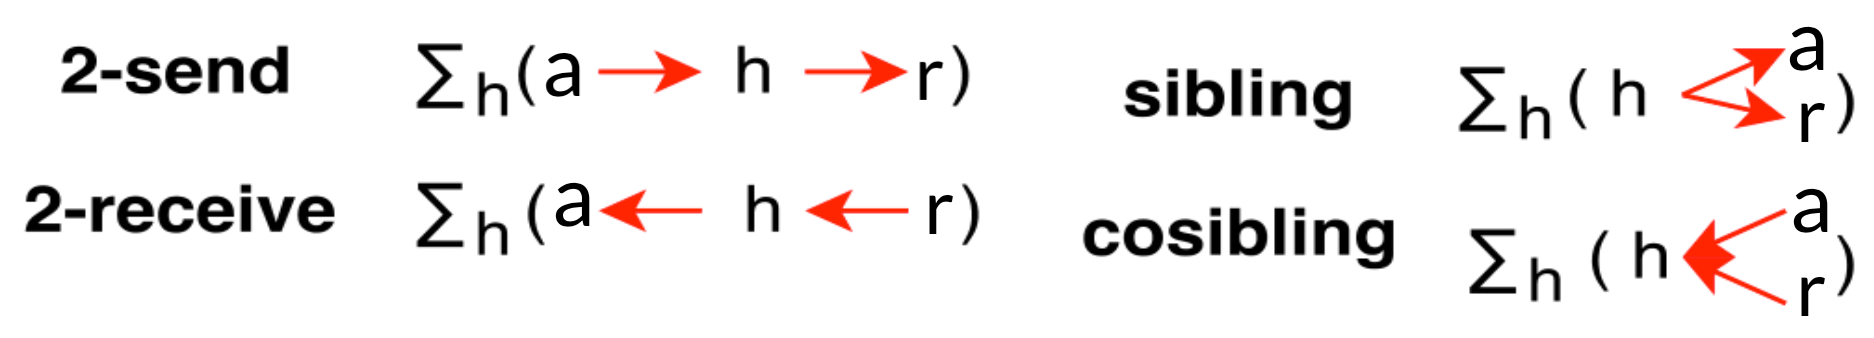
\includegraphics[width=0.6\textwidth]{img/triad-1.png}	
 	   	\caption {Visualization of triadic statistics: 2-send, 2-receive, sibling, and cosibling.}
 	   	\label{figure:netstats}
 	   \end{figure}
 	   
 	    	   \subsubsection{Timestamp covariates}
 	   For the event timing features $\boldsymbol{y}$ introduced in Section \ref{subsec:Time}, we identify a set of covariates which may possibly effect ``time to the next email." Similar to the edge covariates, we include nodal statistics which are time-invariant (such as gender or manager status) or time-dependent (such as the network statistics used for $\boldsymbol{x}$). In addition, we select some edge-specific covariates based on the temporal aspect of the $(d-1)^{th}$ email---e.g., whether the previous email was sent (1) during the weekend and (2) before or past midday (AM/PM)---since we expect the email interactions within county government to be less active during the weekend and in the evening. To be specific, the timestamp statistics are defined as
 	   \begin{itemize}
 	   	\item[1.] intercept: ${y}_{ad1} =1$;
 	   \item[2.] gender of sender: ${y}_{ad2}=I(\mbox{gender of sender }a= \mbox{female})$;
 	   \item[3.] manager status of sender: ${y}_{ad3}=I(\mbox{sender }a \mbox{ is the County Manager})$;
 	   	\item[4.] outdegree of sender: ${y}_{ad4} =\sum_{d^\prime: t_{d^\prime} \in l_d} I(a_{d^\prime} = a)$;
 	   	\item[5.] indegree of sender: ${y}_{ad5}=\sum_{d^\prime: t_{d^\prime} \in l_d} I(u_{d^\prime a} = 1)$;
 	   	\item[6.] weekend indicator of previous email: ${y}_{ad6} = I(t_{d-1} \mbox{ is during the } \mbox{weekend})$;
 	   	\item[7.] AM/PM of previous email: ${y}_{ad7}= I(t_{d-1} \mbox{ in } \mbox{PM})$.
 	   \end{itemize}
 	   Note that our generative process for timestamps in Section \ref{subsec:Time} is sender-orientd process where the sender deterimes ``when to send the email," thus we incorporate network statistics that depends on $a$ only---outdegree of sender $a$ and indegree of sender $a$ (not $r$ this time).

	\subsection{Model Selection}\label{subsec:Experiment_email}
	
	The HEM has many component parts that need to be specified by the user (i.e., the receiver selection features $\boldsymbol{x}$, the selection of the event timing features $\boldsymbol{y}$, and the distribution of time increments $f$). Many of these components will be specified based on user expertise (e.g., regarding which features would drive receiver selection), but some decisions may require a data-driven approach to model specification. For example, though theoretical considerations may inform the specification of features, subject-matter expertise is unlikely to inform the decision regarding the family of the event time distribution. Furthermore, since different distribution families (and model specifications more generally) may involve different size parameter spaces, any data-driven approach to model comparison must guard against over-fitting the data. In this section we present a general-purpose approach to evaluating the HEM specification using out-of-sample prediction. We illustrate this approach by comparing alternative distributional families for the event timing component of the model. Here, we specifically compare the predictive performance from two distributions---log-normal and exponential. We particularly choose the log-normal distribution based on some exploratory analysis (e.g., histogram and simple regressions) on raw time increments data, and take exponential distribution as an alternative since exponential is the most commonly specified distribution for time-to-event data which is also used in the stochastic actor-oriented models (SAOMs) \citep{snijders1996stochastic} as well as their extensions \citep{snijders2007modeling}. 
	\begin{algorithm}[!t]
		\spacingset{1}
		\caption{Out-of-Sample Predictions}
		\label{alg:PPE}
		\begin{algorithmic}
			\STATE {\bfseries Input}: data $ \{ (a_d, \boldsymbol{r}_d, t_d)\}_{d=1}^D$, 
			number of new data to generate $R$, and initial values of $(\boldsymbol{b}, \boldsymbol{\eta}, \boldsymbol{u}, \sigma^2_\tau)$
			\vskip 0.1in
			\textbf{Test splits} (with $p=0.1$):	
			\STATE draw test senders (out of $D$ senders) 
			\STATE draw test receivers (out of $D\times (A-1)$ receiver indicators $\{\{\boldsymbol{r}_{dr}\}_{r\in [A]_{\backslash a_d}}\}_{d=1}^D$)
			\STATE draw test timestamps  (out of $D$ timestamps) 
			\STATE set the test data as ``missing" (NA)
			\vskip 0.1in
			\textbf{Imputation and inference:}	
			\FOR{$r=1$ {\bfseries to}  $R$}
			\FOR{$d=1$ {\bfseries to}  $D$}
			\IF{$a_d=$  NA}
			\FOR{$a=1$ {\bfseries to} $A$}
			\STATE compute $\pi_{a}=P(a_d= a | \cdot)$ using equation (\ref{eqn:latenttime}) (without the product term)
			\ENDFOR
			\STATE draw $a_d \sim \mbox{multinomial}(\pi_a)$
			\ENDIF
			\FOR{$r\in [A]_{\backslash a_d}$}
			\IF{$r_{dr}=$ NA}
			\STATE draw $r_{dr}$ from multinomial with probability $P(r_{dr}= 1 | \cdot)$ and $P(r_{dr}= 0| \cdot)$ using equation (\ref{eqn:latentreceiver})
			\ENDIF
			\ENDFOR
			\IF{$t_d=$ NA}
			\STATE draw $\boldsymbol{\tau}^{new}_d$ from equation (\ref{eqn:latenttime}) (without the product term) via importance sampling\footnote{we need to specify appropriate proposal distribution such as $g \sim \mbox{halfcauchy}(5)$}
			\ENDIF
			\STATE run inference and update $(\boldsymbol{u},\boldsymbol{b}, \boldsymbol{\eta})$ given the imputed and observed data
			\ENDFOR
			\STATE store the estimates for test data
			\ENDFOR
		\end{algorithmic}
	\end{algorithm}
	
	We evaluate the model's ability to predict edges and timestamps from Montgomery County email data, conditioned on their ``training" part of the data. To perform the experiment, we separately formed a test split of each three model components---sender, receivers, and timestamps---by randomly selecting ``test" data with probability $p=0.1$. Any missing variables were imputed by drawing samples from their conditional posterior distributions, given the observed data, model estimates, and current values of test data. We then run inference to update the latent variables given the imputed and observed data. We iterate the two steps---imputation and inference---multiple times to obtain enough number of estimates for test data. Algorithm \ref{alg:PPE} outlines this procedure in detail. 
	
	We run the experiment and measure the predictive performance of two separate time distributions using $N=500$ predicted samples, by comparing the predictions in terms of classification accuracy in predicting the senders and receivers, as well as prediction error in the timestamps. First, we compare the posterior probability of correct senders for each of missing emails $\{d:a_d=\mbox{NA}\}$, which corresponds to $\pi_{a_{d}}=P(a_{d} = a^{obs}_{d}|\cdot)$ in Algorithm \ref{alg:PPE}. We call this measure as ``correct sender posterior probability." On the left of Figure \ref{figure:PPEresults}, we draw boxplots for the distribution of mean correct sender posterior probability---i.e., $\hat{\pi}_{a_{d}} = \frac{1}{N}\sum_{n=1}^N \pi^n_{a_{d}}$---across the missing emails. The results show that both log-normal and exponential distributions acheive better predictive performance for missing senders compared to what is expected under random guess (i.e., choose one out of $A$ possible senders $=1/18$), with log-normal distribution showing slightly higher performance than exponential distribution on average. Secondly, since the receiver vector is binary, we compute $F_1$ scores for missing receiver indicators (i.e., all $d$ and $r$ with $r_{dr}$=NA) by taking the harmonic mean of precision and recall:
	\begin{equation}
	\begin{aligned}
	F_1 =2\cdot\frac{\mbox{precision}\cdot \mbox{recall}}{\mbox{precision}+ \mbox{recall}}, &\mbox{ where } \\
			\mbox{recall}  = \frac{\mbox{TP}}{\mbox{TP+FN}} \mbox{ and } \mbox{precision} & =\frac{\mbox{TP}}{\mbox{TP+FP}},
			\end{aligned}
	\end{equation}
	with TP denoting true positive (i.e., $\boldsymbol{r}^{obs}_{dr}=\boldsymbol{r}^{pred}_{dr}=1$), FN denoting false negative (i.e., $\boldsymbol{r}^{obs}_{dr}=1$ but $\boldsymbol{r}^{pred}_{dr}=0$), and FP denoting false positive (i.e., $\boldsymbol{r}^{obs}_{dr}=0$ but $\boldsymbol{r}^{pred}_{dr}=1$). Although the generative process for edges (Section \ref{subsec: Tie}) is not directly affected by the choice of timestamp distribution, the middle plot in Figure \ref{figure:PPEresults} reveals noticeable difference between log-normal and exponential in their performance in predicting missing receiver indicators, where log-normal outperforms exponential. Finally, the prediction error for $d^{th}$ missing timestamp is estimated using the median of absolute relative errors\footnote{\cite{hyndman2006another} refer to this as median absolute percentage error (MdAPE).} across $N=500$ predictions:
			\begin{figure}[!t]
				\centering
				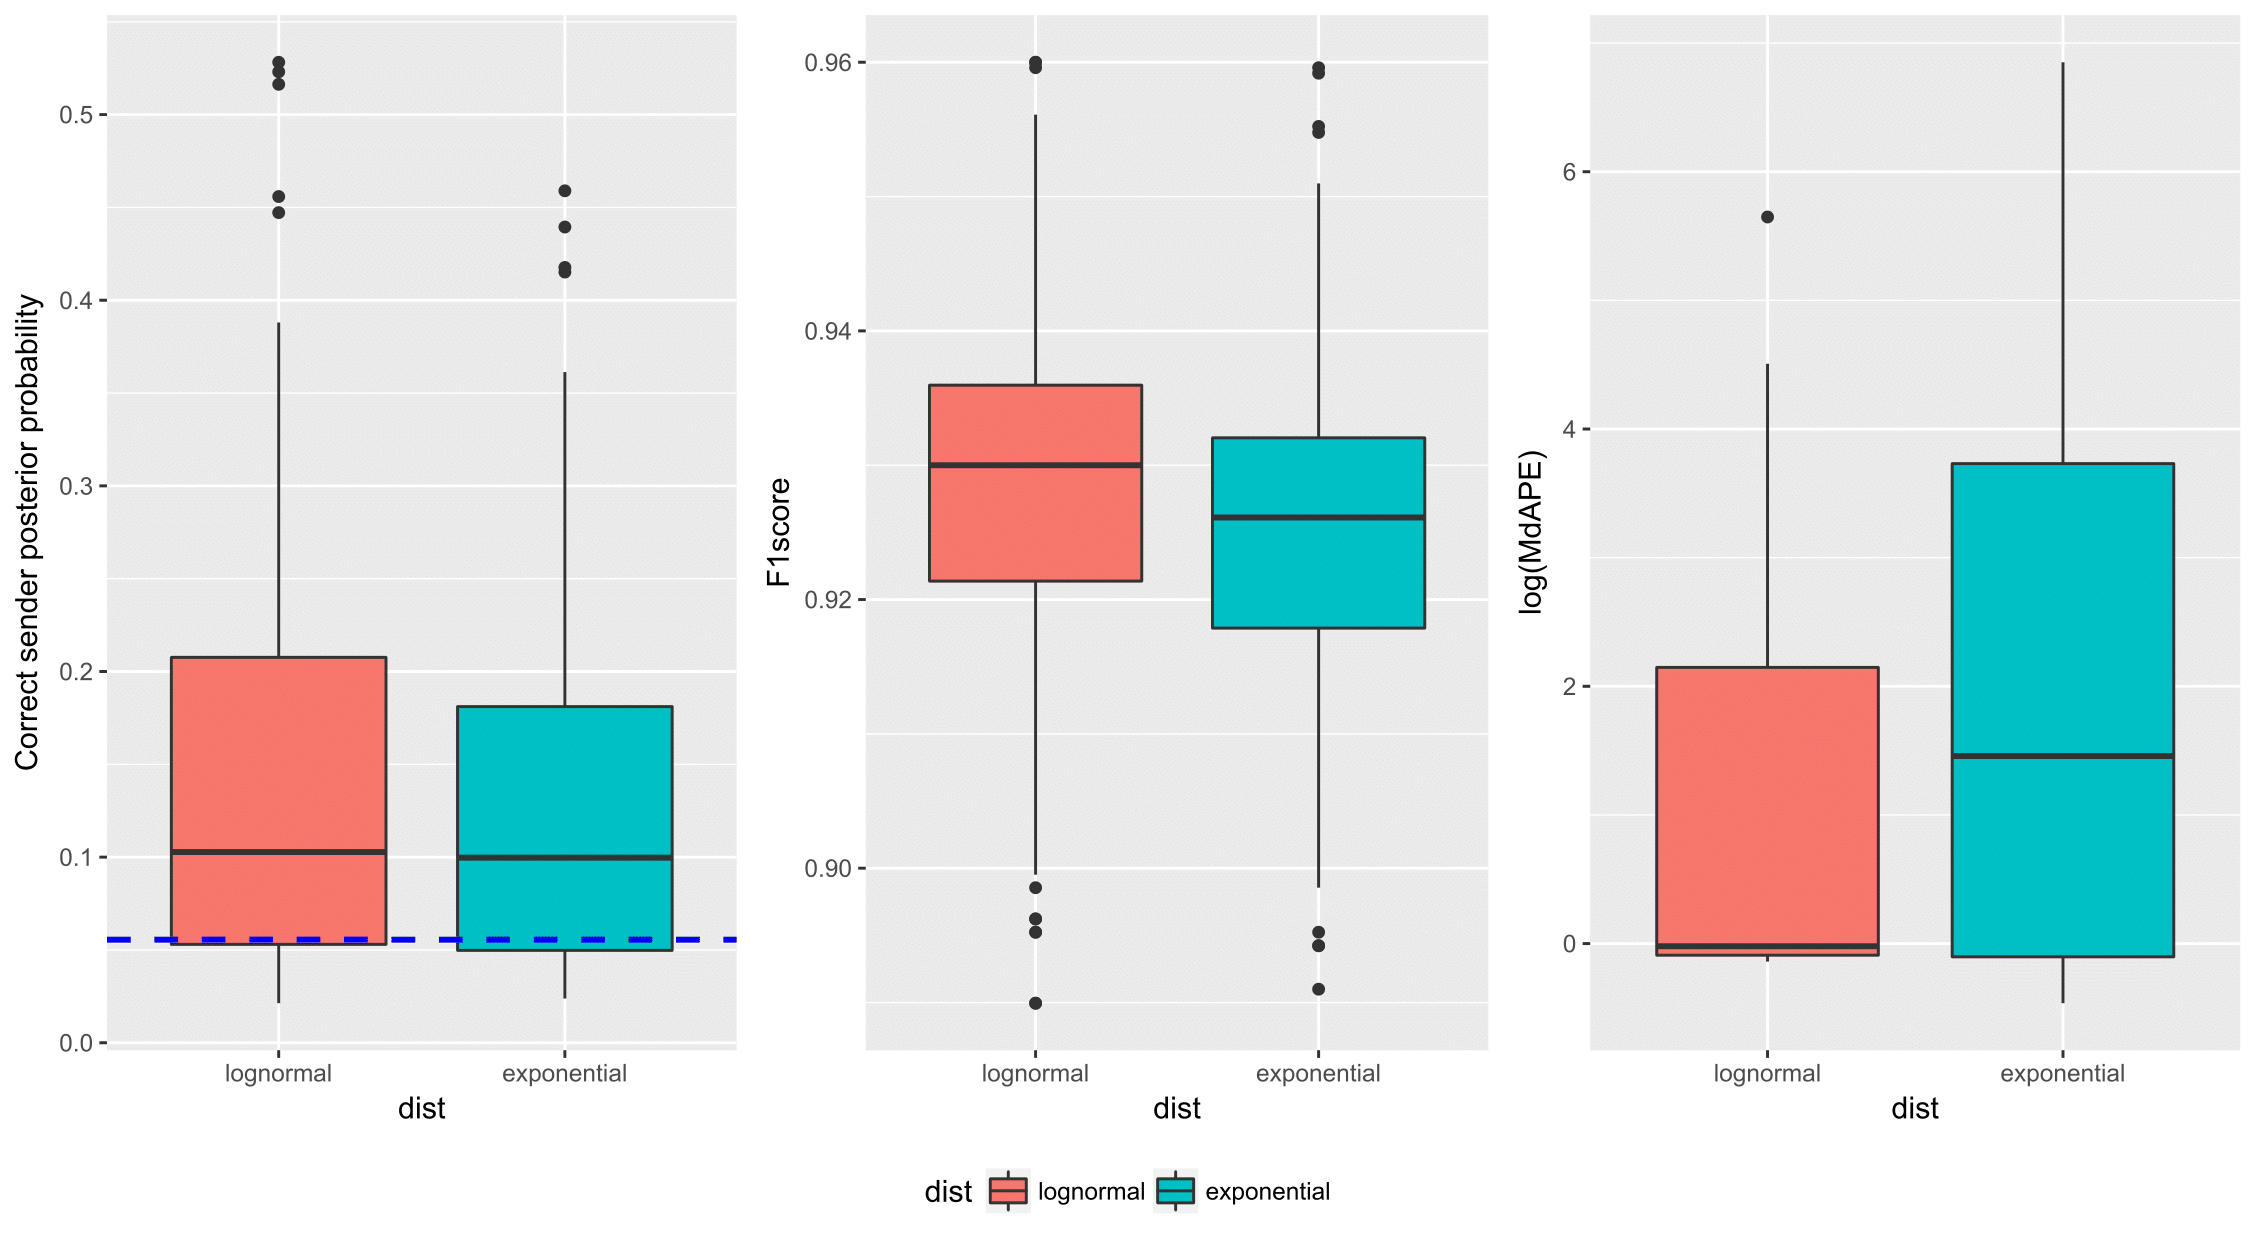
\includegraphics[width=1\textwidth]{img/PPEplotnew-1.png}	
				\caption {Comparison of predictive performance between log-normal and exponential distributions: boxplots for correct sender posterior probability (\textit{left}), $F_1$ scores from receiver predictions (\textit{middle}), and boxplots for median absolute percentage error (\textit{right}). The dotted blue lines in the left plot represents the correct sender probability expected by random guess---i.e., $1/A=1/18\approx0.056$.}
				\label{figure:PPEresults}
			\end{figure}
		\begin{equation}
		e_{\tau_d} = \mbox{median}\Big(\abs*{\frac{\tau^{obs}_d - \tau^{pred_1}_{d}}{\tau^{obs}_d}},\ldots, \abs*{\frac{\tau^{obs}_d - \tau^{pred_N}_{d}}{\tau^{obs}_d}}\Big).
		\end{equation}
	The right plot of Figure \ref{figure:PPEresults} presents boxplots for the median absolute relative errors. where plot the estimates in a log-scale. Surprisingly, we have a huge benefit in the performance of timestamp prediction when we assume log-normal distribution for time-increments compared to exponential distribution. This difference can be explained by overdispersion in exponential distribution, because there exists greater variability in the time increments of emails than would be expected under exponential distribution. As illustrated above, we can use this out-of-sample prediction task for two usage---1) provide an effective answer to the question ``how are we filling in the missing components of time-stamped network data?" and 2) offer one standard way to determine the distribution of time increments in Section \ref{subsec:Time}. 

	\subsection{Posterior Predictive Checks}\label{subsec:PPC_email} 	   
In this section, we perform posterior predictive checks (PPC) \citep{rubin1984bayesianly} to evaluate the appropriateness of our model specification for Montgomery County email data. We formally generated entirely new data, by simulating $N=500$ synthetic email data $\{(a_{d}, \boldsymbol{r}_{d}, t_{d})\}_{d=1}^D$ from the genenerative process in Section \ref{sec:generative process}, conditional upon a set of inferred latent variables from the inference in Section \ref{subsec:Result_email}\iffalse, where the pseudocode is outlined in Algorithm \ref{alg:PPC}\fi. For the test of goodness-of-fit in terms of network dynamics, we use multiple statistics that summarize meaningful aspects of the data: outdegree distribution, indegree distribution, receiver size distribution, and probability-probability (PP) plot for time increments. 
\iffalse
	\begin{algorithm}[!t]
		\spacingset{1}
		\caption{Generate new data for PPC}
		\begin{algorithmic}
			\STATE \textbf{Input}: number of data to generate $R$, covariates $(\boldsymbol{x},\boldsymbol{y})$, and estimated values of $(\boldsymbol{u}, \boldsymbol{b}, \boldsymbol{\eta})$\\
			\vskip 0.1in
			
			\FOR{$r=1$ {\bfseries to}  $R$}
			\FOR{$d = 1$ {\bfseries to}  $D$} 
			\STATE	Draw ($a_{d}$, $\boldsymbol{r}_{d}$, $t_{d}$) following Algorithm \ref{alg:generative}\\
			\ENDFOR
			\STATE Store every $r^{th}$ new data $\{(a_{d}, \boldsymbol{r}_{d}, t_{d})\}_{d=1}^D$ 
			\ENDFOR
		\end{algorithmic}
		\label{alg:PPC}
	\end{algorithm}     \fi  
		
	Figure \ref{figure:PPCresults} illustrates the results of poterior predictive checks using log-normal distribution, which shows better performance in Section \ref{subsec:Experiment_email}. Upper two plots show node-specific posterior predictive degree distributions across $N=500$ synthetic data, where the left one for outdegree statistic and the right plot is for indegree statistic. For both plots, the x-axis represents the nodes ($A=1,\ldots,18$), and the y-axis represents the number of emails sent or received by the node. When compared with the observed outdegree and indegree statistics (red lines), our model recovers the overall distribution of sending and receiving activities across the nodes. For example, node 1 and 10 show significantly higher level of both sending and receiving activities relative to the rest, and the model-simulated data captures those big jumps, showing acceptable fit to the data. Outdegree distribution of some low-activity nodes are not precisely recovered, however, indegree distribution looks much better. Since we use more information in the receiver selection process (i.e., network effects) while we rely solely on minimum time increments when choosing the observed sender, these results are expected. Lower left plot is the distribution of receiver sizes, where the x-axis spans over the size of receivers 1 to 14 (which is the maximum size of observed receivers) and the y-axis denotes the number of emails with x-number of receivers. The result shows that our model is underestimating emails with one receiver while overestimating emails with two, three, and four receivers. One explanation behind what we observe is that the model is trying to recover so-called ``broadcast'' emails, which are the emails with $\geq 10$ number of receivers, so that the intercept estimate $b_1$ is slightly moved toward right. To improve the goodness of fit for receiver sizes, we can add more covariates (e.g., sender indicators) or assign strong prior structure on $b_1$. In the end, the plot on the lower right is the PP plot for time increments, which depicts the two cumulative distribution functions---one for simulated time increments and another for observed time increments---against each other in order to assess how closely two data sets agree. Here, the closeness to the diagonal line connecting $(0, 0)$ and $(1, 1)$ gives a measure of difference between the simulated and observed time increments, and our PP plot shows that we have great performance in reproducing the observed time distribution. All our findings from predictive experiments in Section \ref{subsec:Experiment_email} are further revealed in the PPC from exponential distribution, where the PPC plots comparing log-normal and exponential distributions are attached in Appendix C.
	\begin{figure}[!htb]
		\centering
		\begin{tabular}[t]{cc}
		   	\begin{subfigure}[b]{0.495\textwidth}
		   		\caption{Outdegree distribution}
		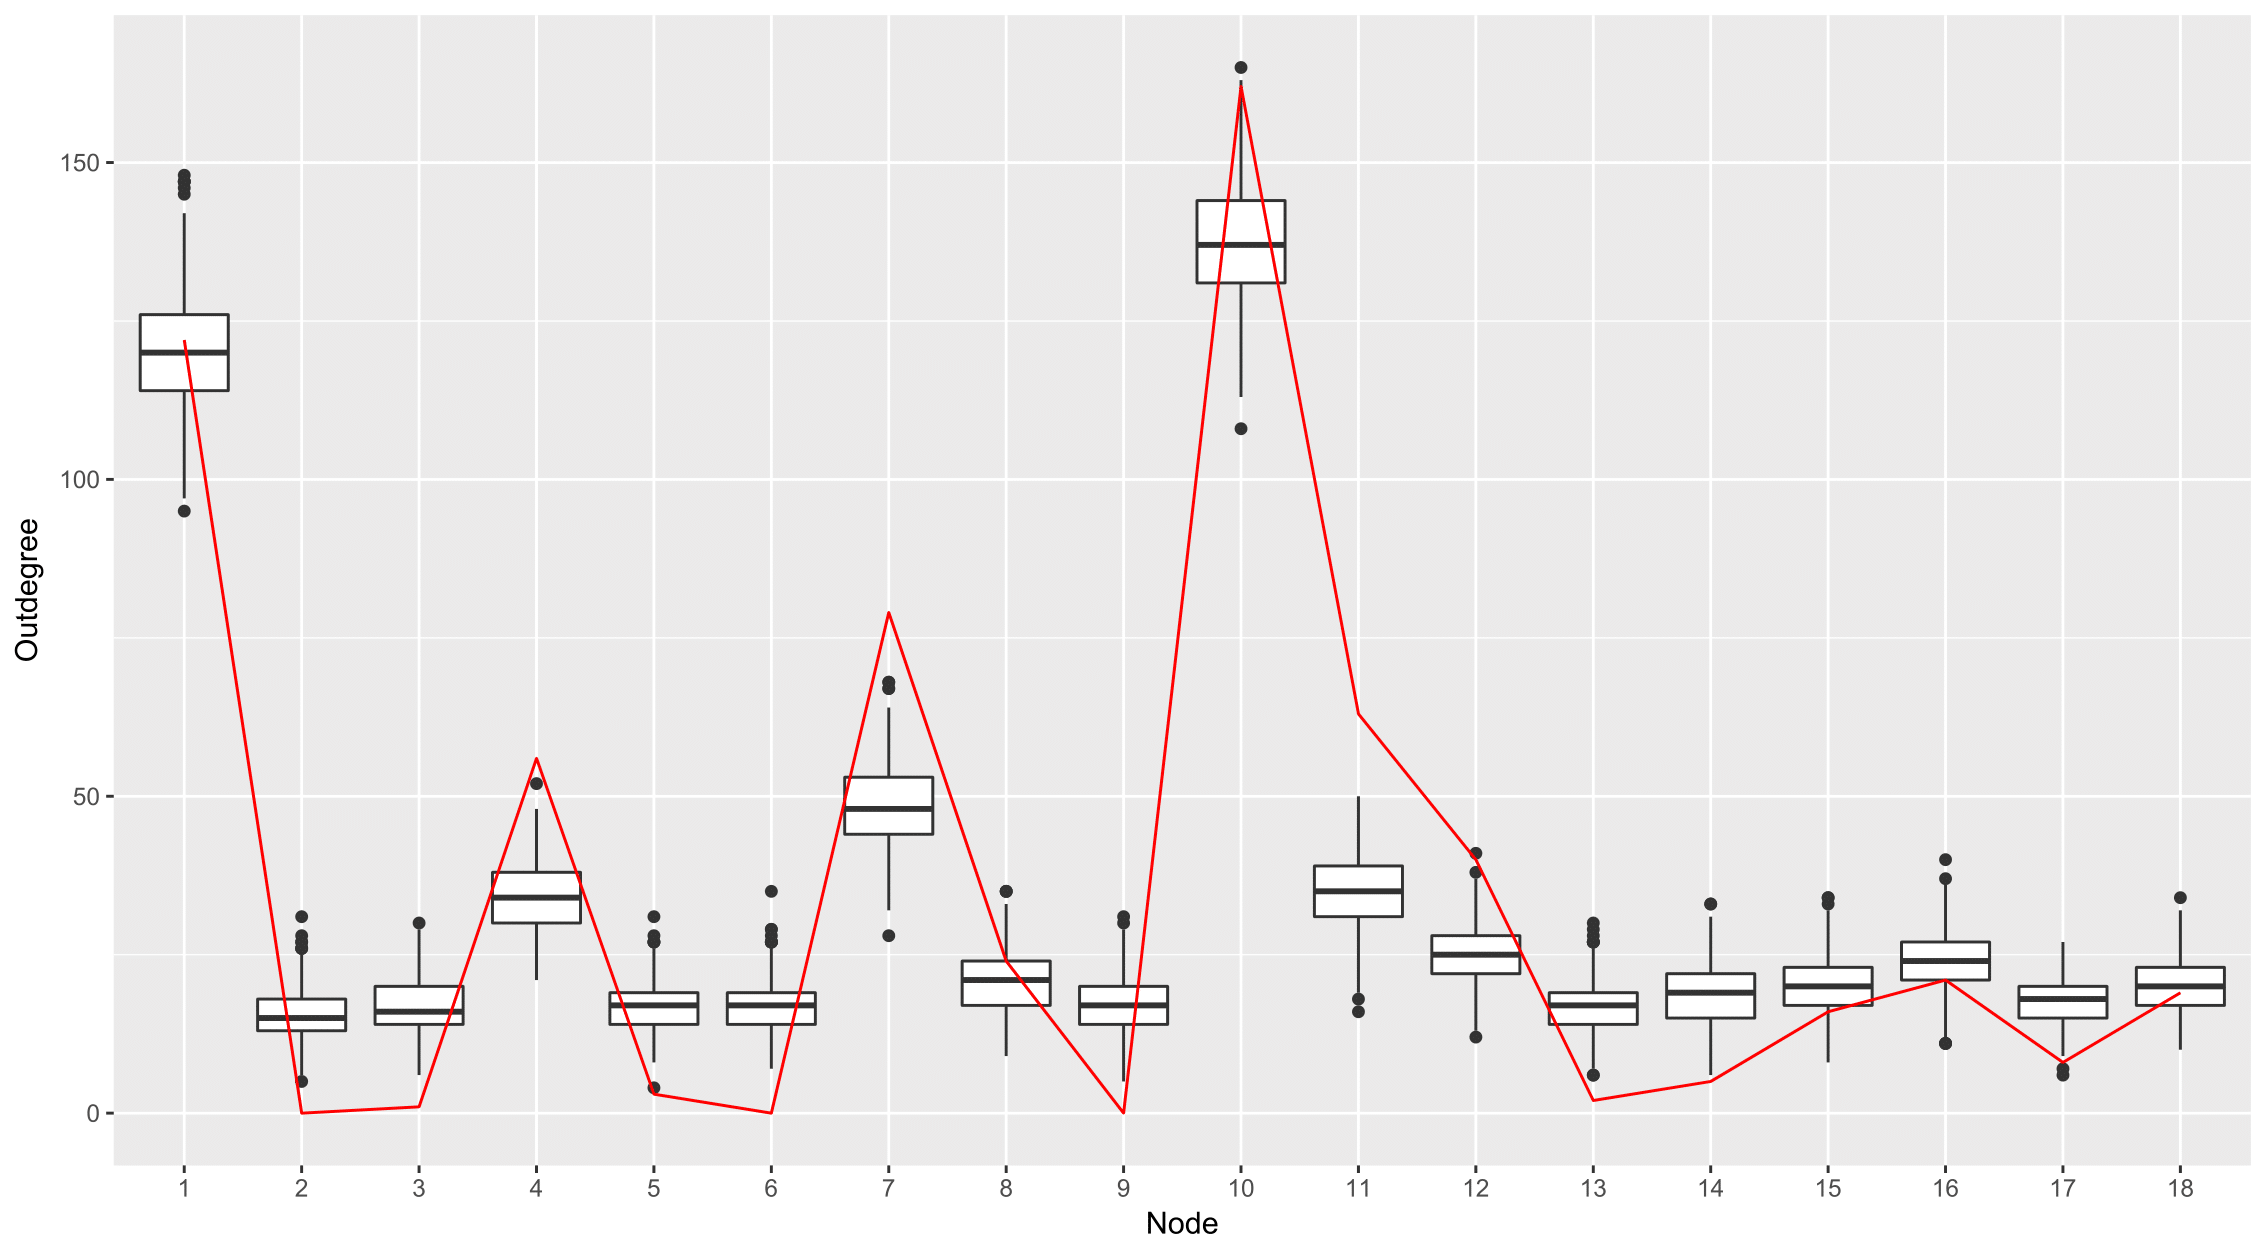
\includegraphics[width=\textwidth]{img/outdegreenew-1.png}	
		   	\end{subfigure}
		   			   	\begin{subfigure}[b]{0.495\textwidth}
		   			   		\caption{Indegree distribution}
		   			   		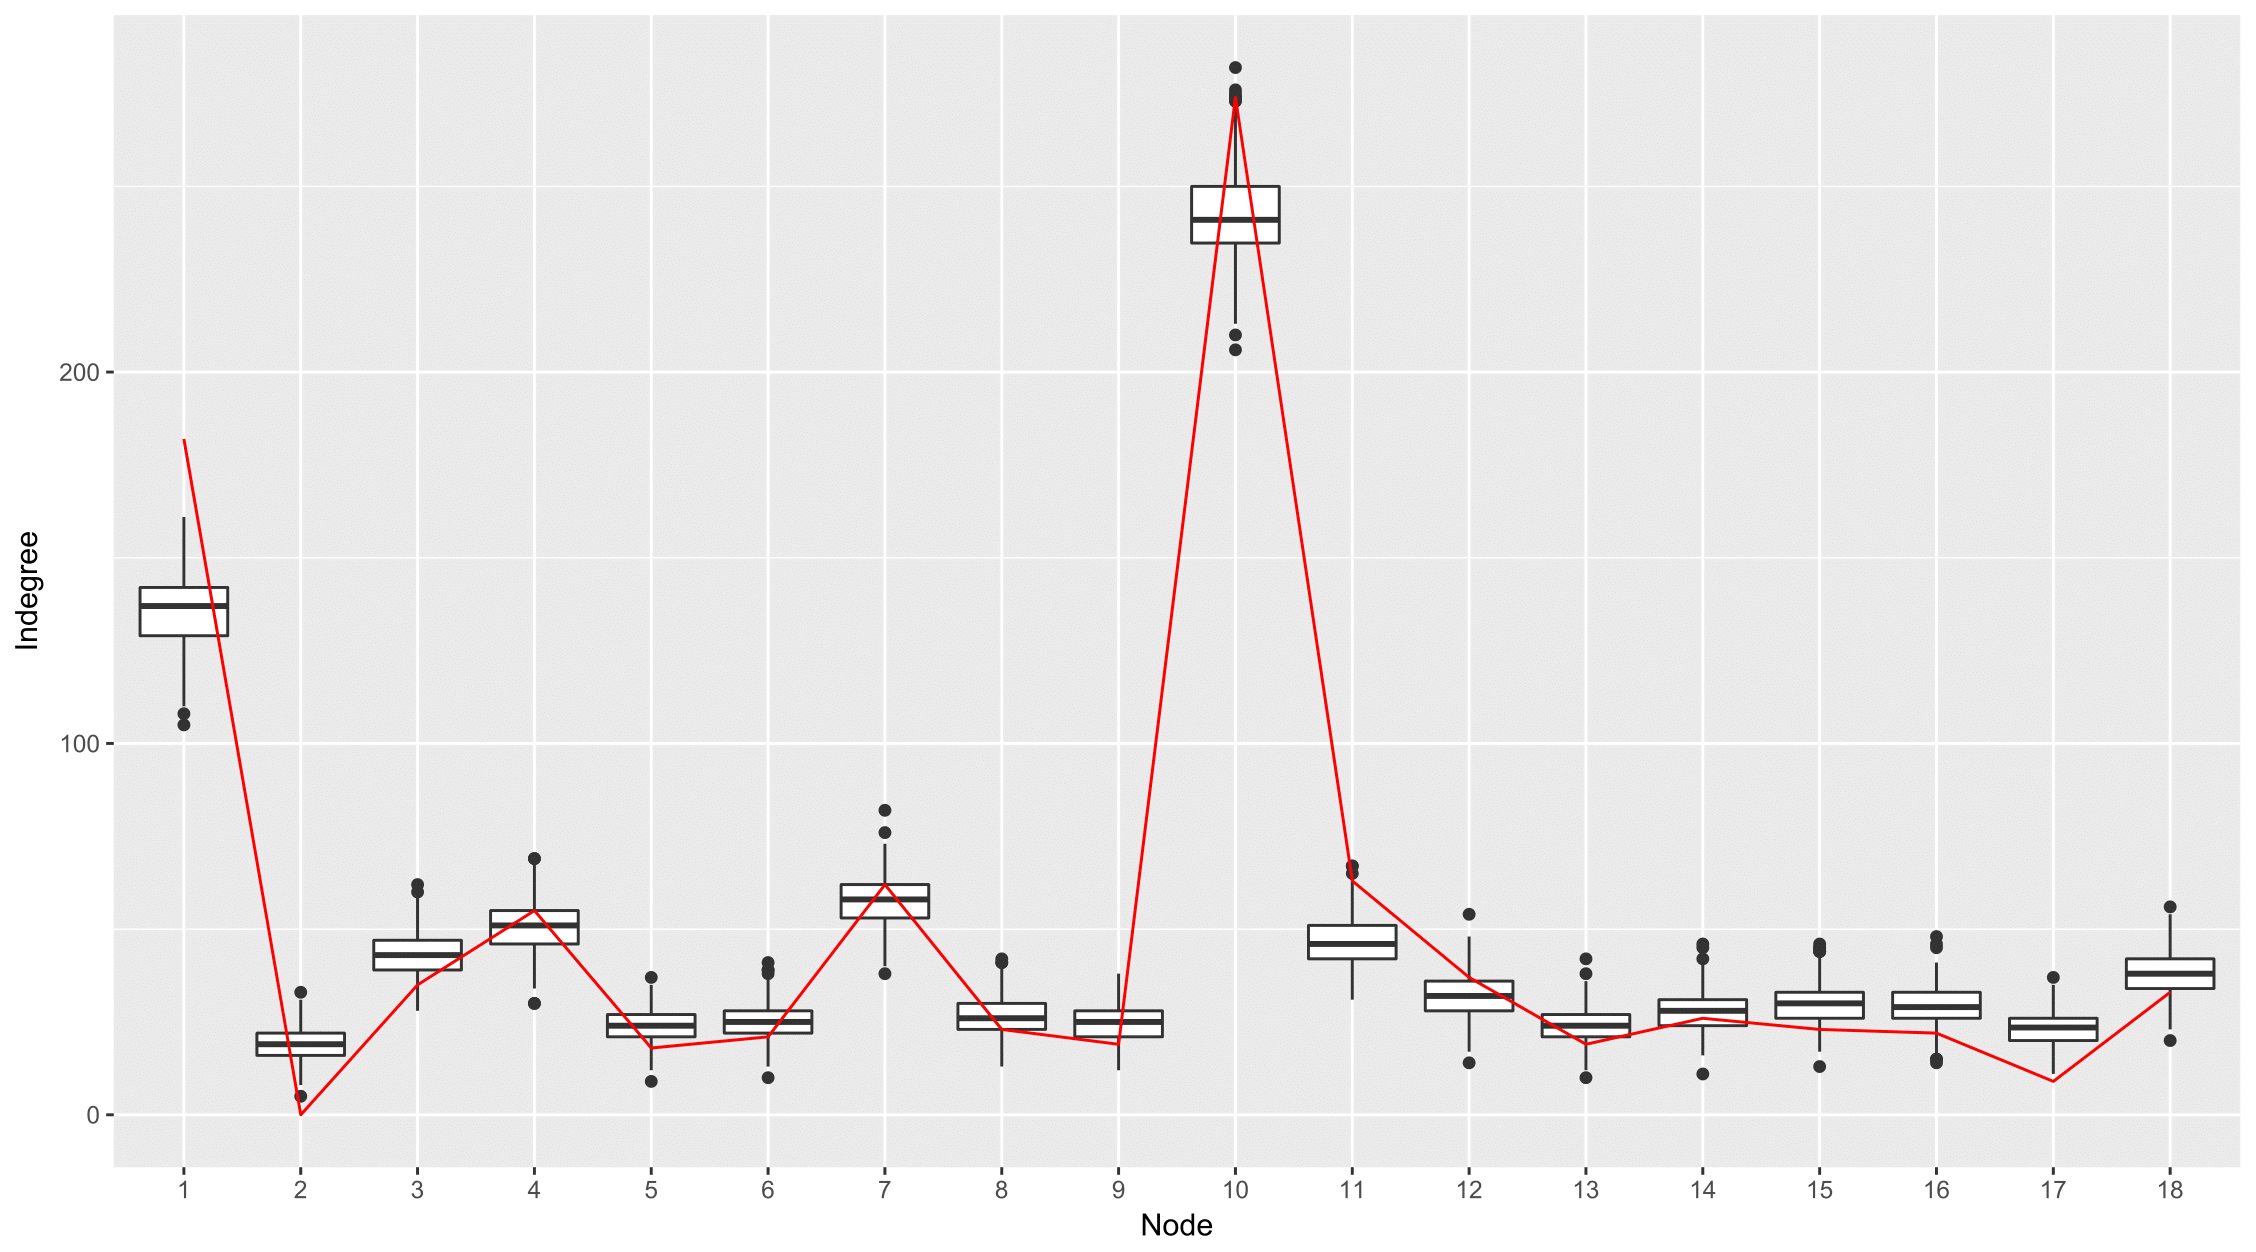
\includegraphics[width=\textwidth]{img/indegreenew-1.png}	
		   			   	\end{subfigure}\\
			   	\begin{subfigure}[b]{0.495\textwidth}
			   		\caption{Receiver size distribution}
			   		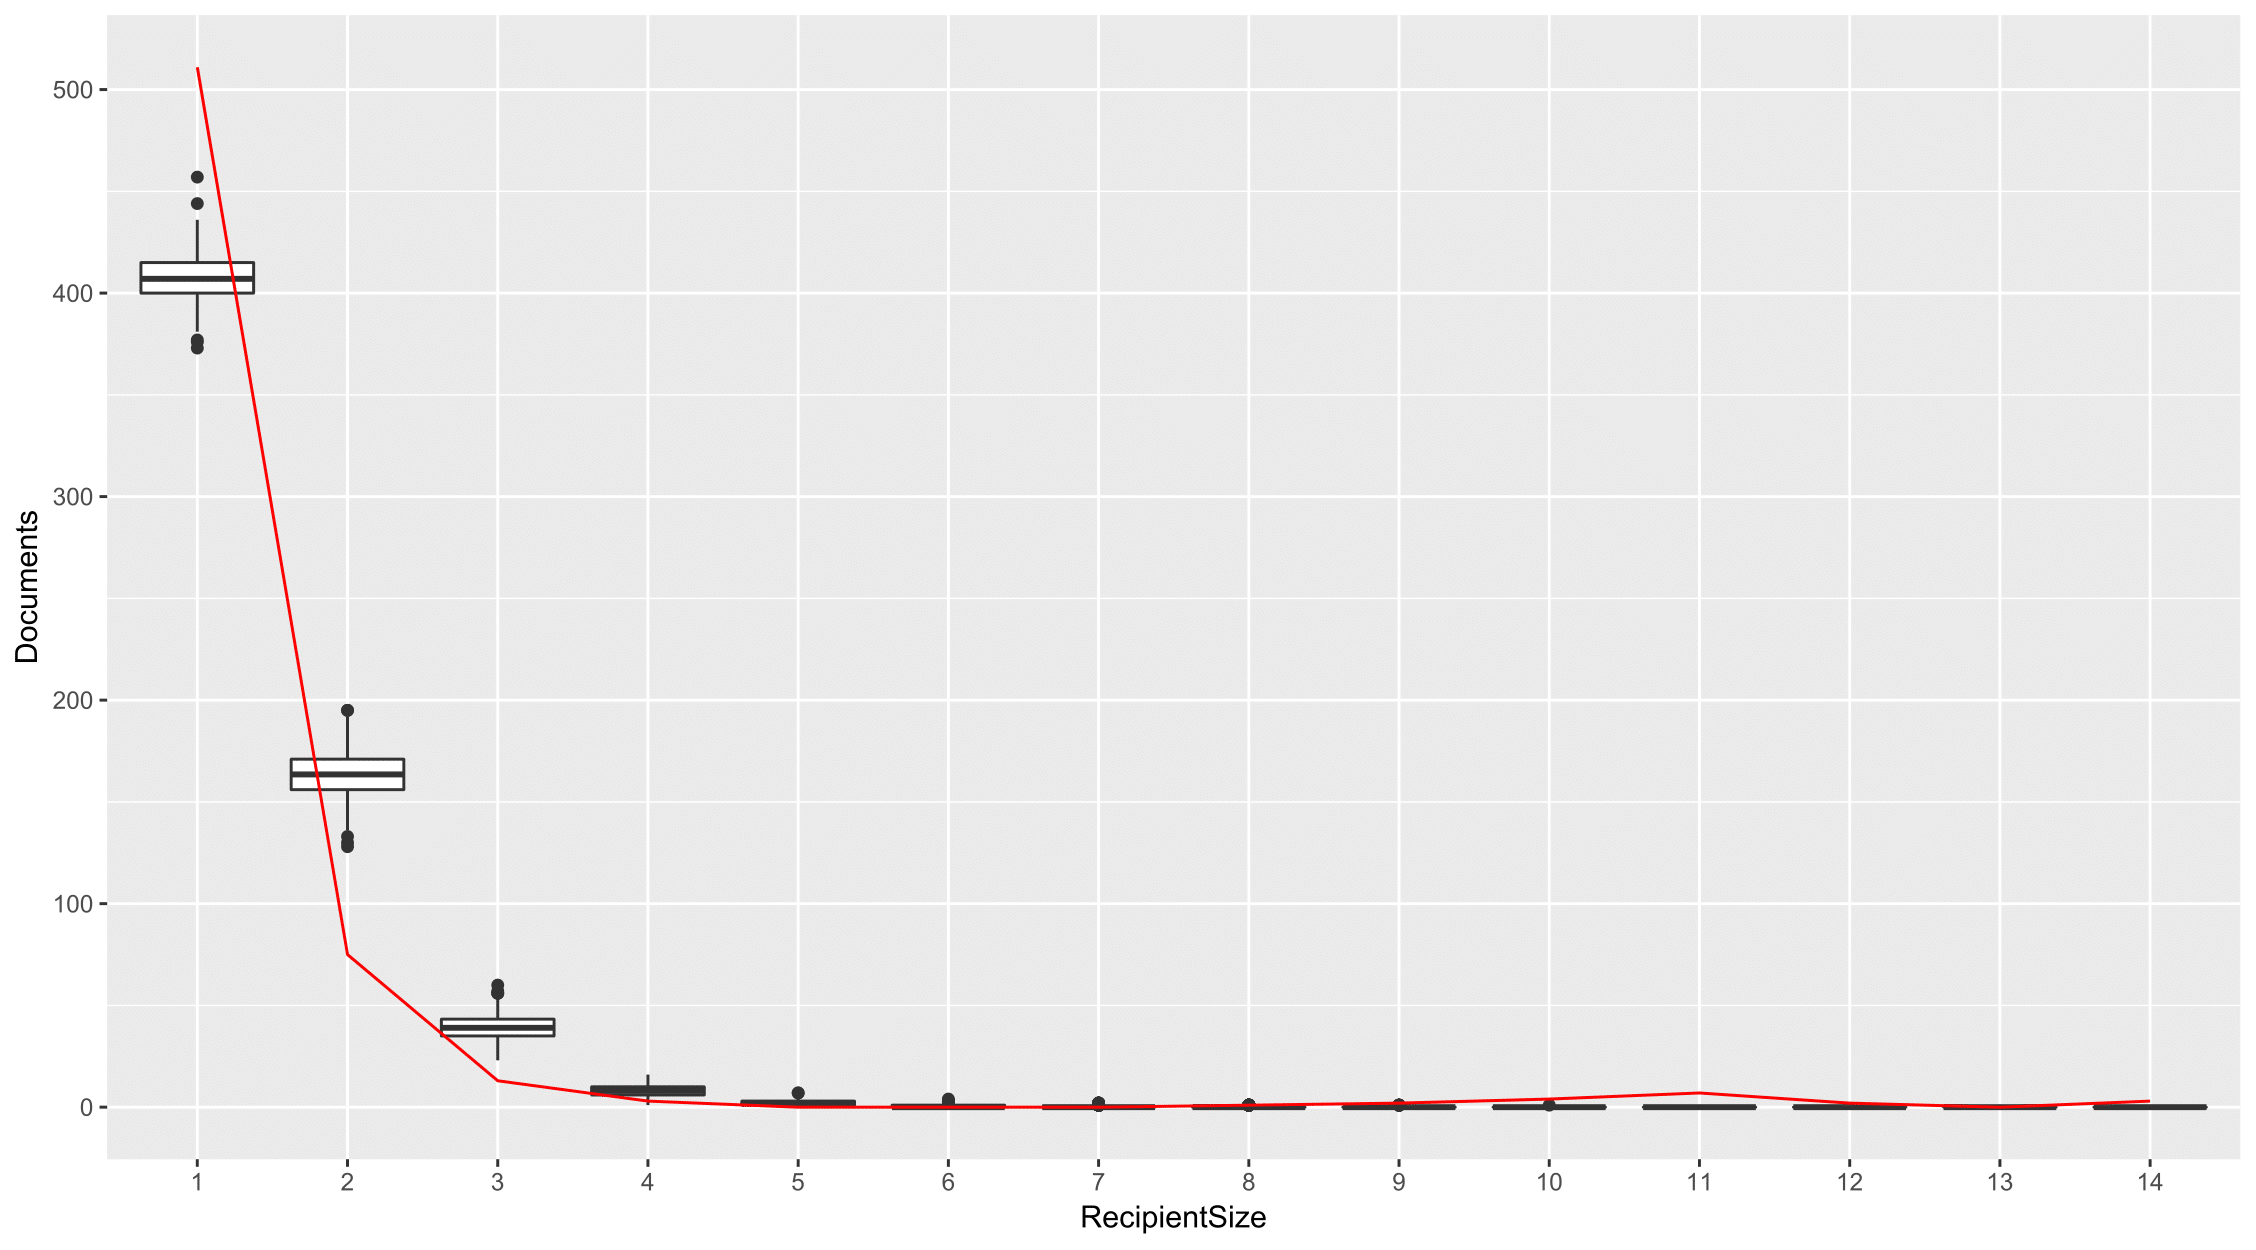
\includegraphics[width=\textwidth]{img/recipientsizenew-1.png}	
			   	\end{subfigure}
			   	\begin{subfigure}[b]{0.495\textwidth}
			   				\centering
			   		\caption{PPplot for time increments}
			   		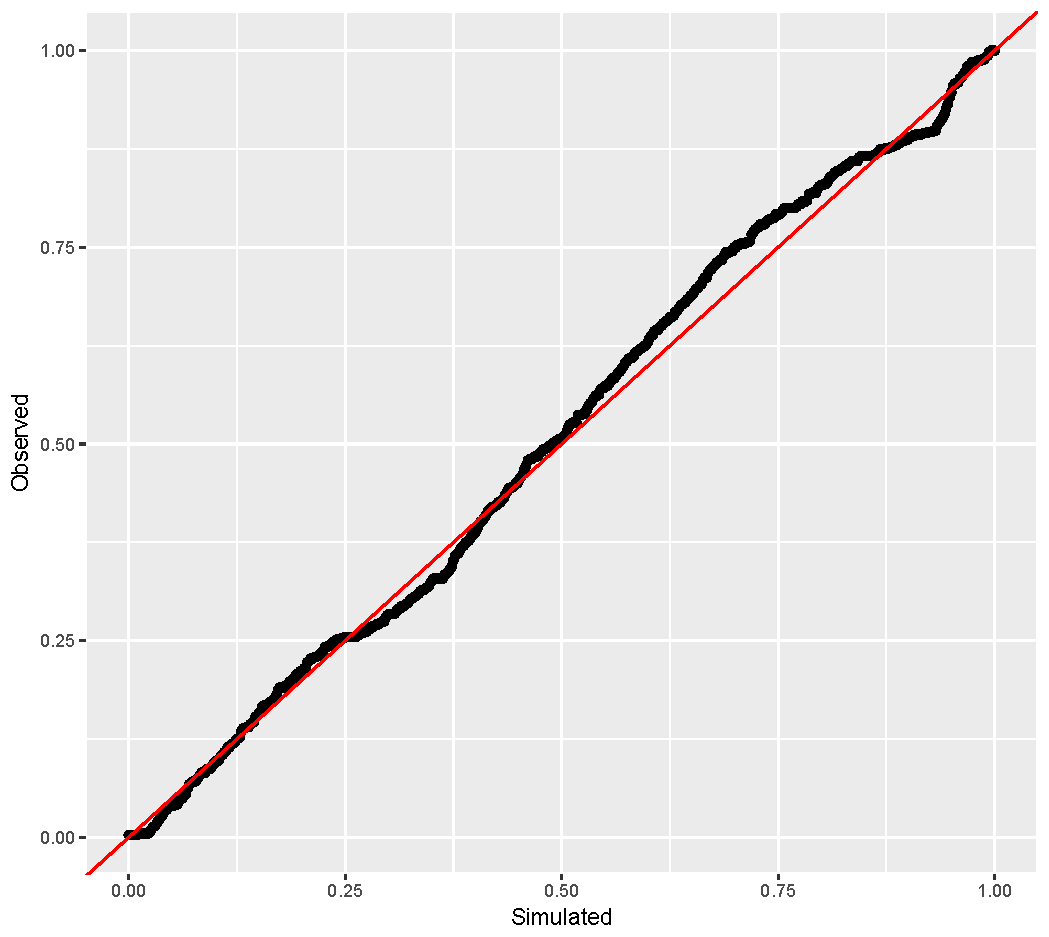
\includegraphics[width=0.625\textwidth]{img/timeppnew.pdf}	
			   	\end{subfigure}
		\end{tabular}
		\caption {PPC results from log-normal distribution. Blue lines denote the observed statistics in (a)--(c) and denotes the diagonal line in (d).}
		\label{figure:PPCresults}
	\end{figure}
	
	\subsection{Exploratory Analysis}\label{subsec:Result_email}
	Based on the prediction experiments in Section \ref{subsec:Experiment_email}, we choose to analyze Montgomery county email data and interpret the results using log-normal distribution. We assume weakly informative priors for latent variables such as $\boldsymbol{b}\sim N(\boldsymbol{\mu}_b=\boldsymbol{0}, \Sigma_b = 2\times I_P)$, $\boldsymbol{\eta}\sim N(\boldsymbol{\mu}_\eta=\boldsymbol{0}, \Sigma_\eta = 2\times I_Q)$, and $\sigma_\tau^2 \sim \mbox{inverse-Gamma}(a=2, b=1)$, and run MCMC algorithm in Algorithm \ref{alg:MCMC} with $O=55,000$ outer iterations with a burn-in of 15,000, where we thin by keeping every 40th sample. While the inner iterations for $\sigma_\tau^2$ is fixed as 1, we specify the inner iterations $I_1=20$ for $\boldsymbol{b}$ and $I_2=10$ for $\boldsymbol{\eta}$ to adjust for slower convergence rates. Convergence diagnostics including the traceplots and Geweke diagnostics \citep{geweke1991evaluating} are provided in Appendix D.
	\begin{figure}[!t]
		\centering
		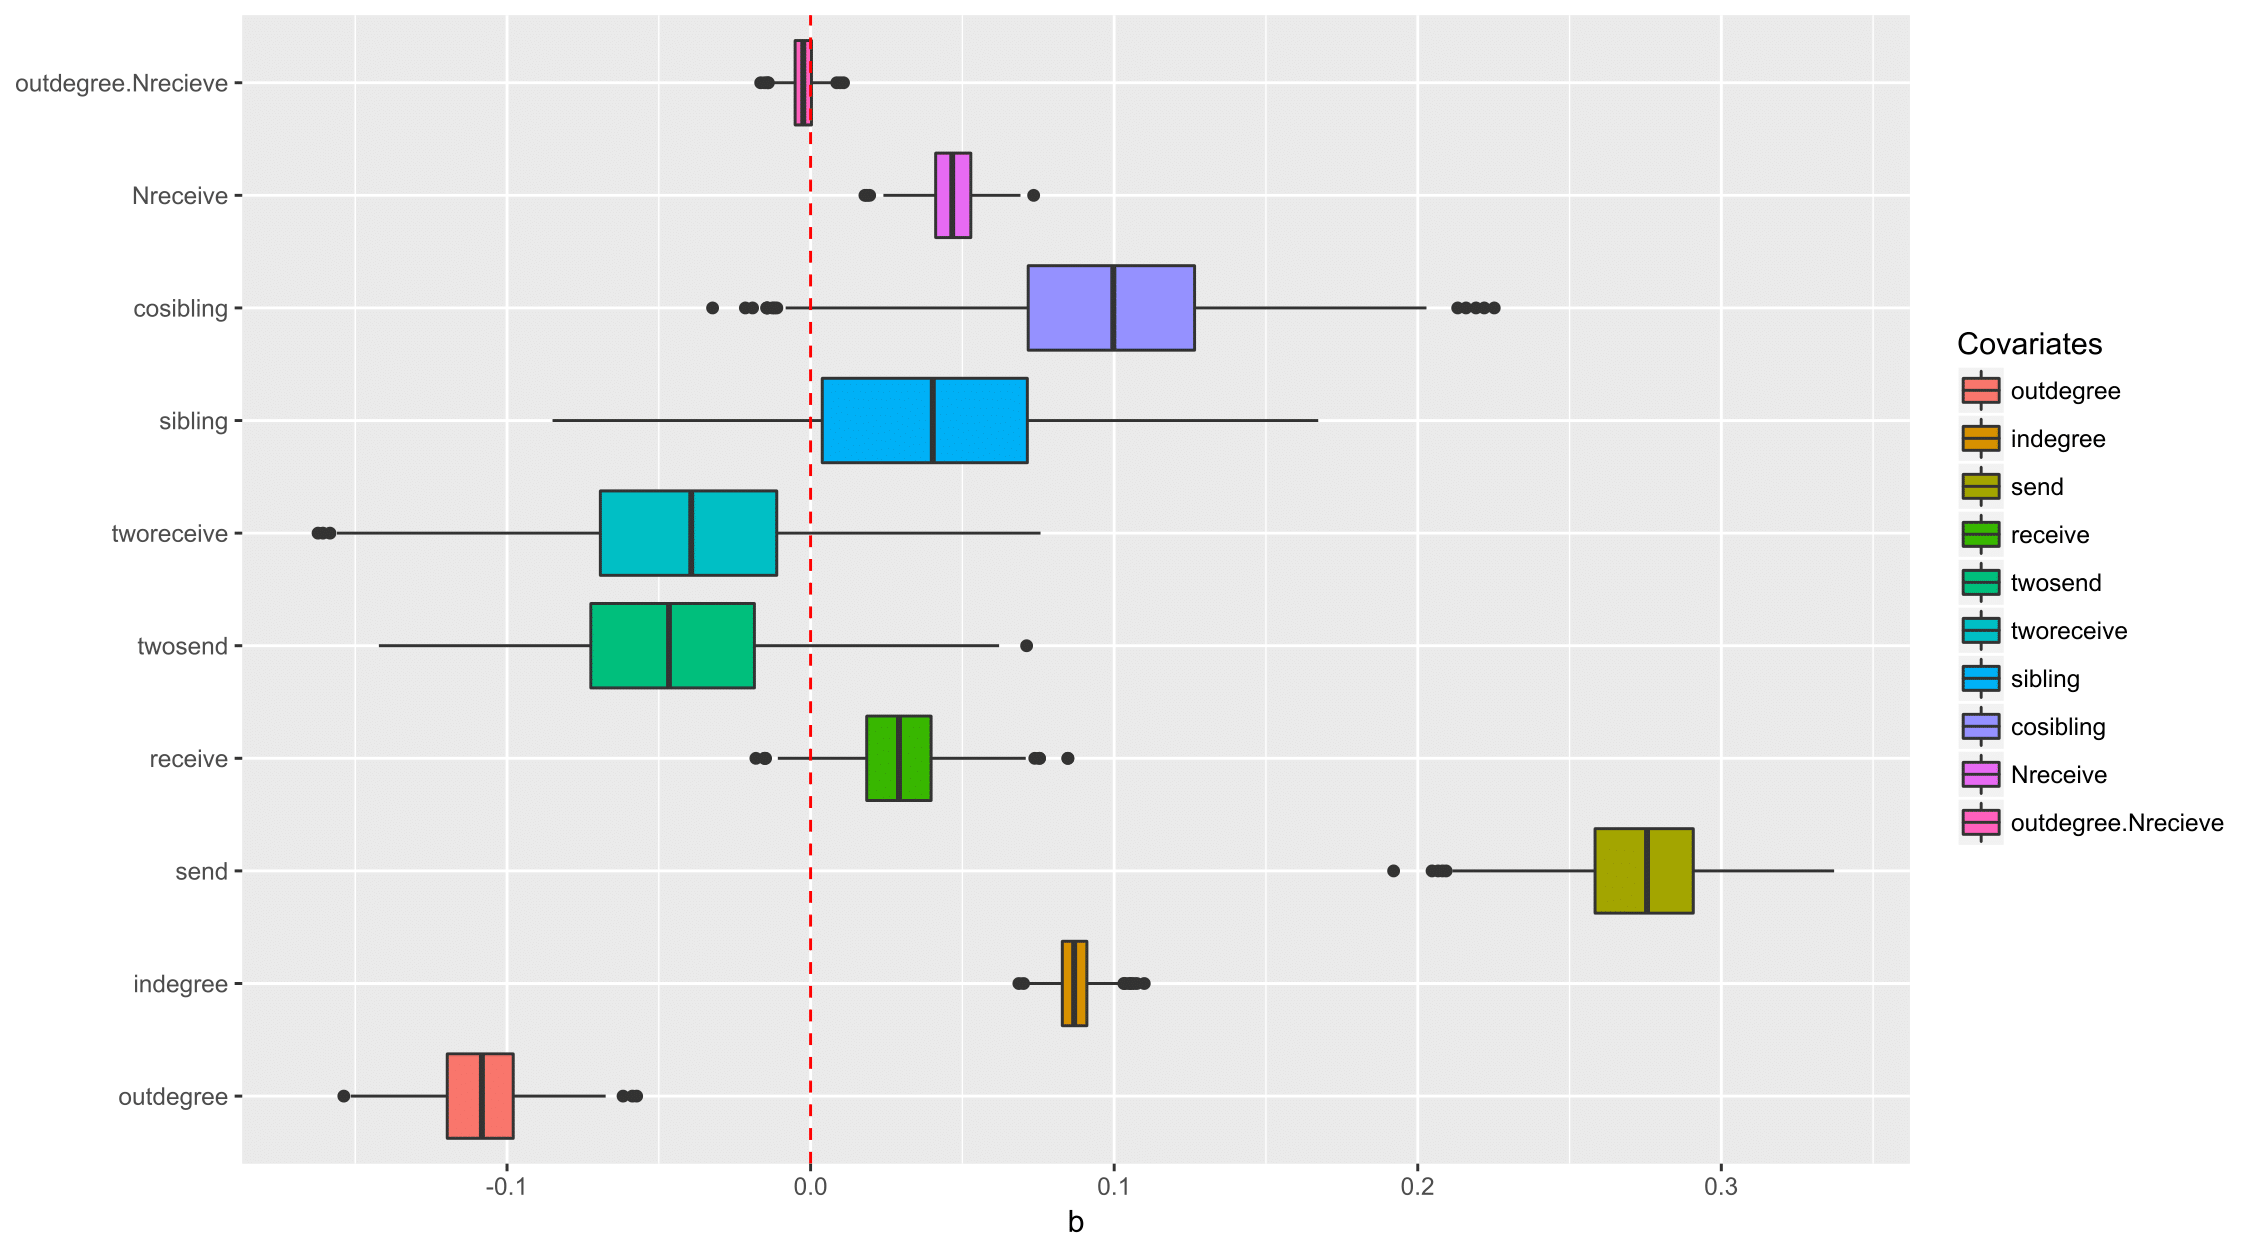
\includegraphics[width=1\textwidth]{img/best-1.png}	
		\caption {Posterior distribution of $\boldsymbol{b}$ estimates.}
		\label{figure:betaresults}
	\end{figure}
	\subsubsection{Coefficients for edge covariates}
	Figure \ref{figure:betaresults} shows the boxplots summarizing posterior samples of $\boldsymbol{b}$. Since we use the logit probability of $\lambda_{adr}$ when generating hypothetical edges in Section \ref{subsec: Tie}, we assume that 
	\begin{equation*}
	\mbox{logit}(\lambda_{adr})=\log\Big(\frac{\lambda_{adr}}{1-\lambda_{adr}}\Big) =b_{1}+b_{2} x_{adr2}\ldots+b_{14}x_{adr14},
	\end{equation*}
	and can interpret the $\boldsymbol{b}$ estimates in terms of odds ratio $\frac{\lambda_{adr}}{1-\lambda_{adr}}=\exp(b_{1}+b_{2} x_{adr2}\ldots+b_{14}x_{adr14})$.
	To begin with, we can see that the effect of the statistic``send" (i.e., number of times sender $a$ sent emails to receiver $r$ over the last week) is significant and positive with $\hat{b}_4 = 0.274$, implying that if sender $a$ sent $n$ number of emails to $r$ last week, then sender $a$ is approximately $\exp(0.274\times n)\approx(1.315)^n$ times more likely to send an email to $r$. Similar interpretation can be applied for the covariates ``indegree" and ``hyperedge size". For example, if the receiver $r$ received $n$ number of emails and sender $a$ sent emails to $n$ number of rececievers over the last week, sender $a$ is $\exp(0.086\times n)\approx(1.091)^n $ times and $\exp(0.047\times n)\approx(1.048)^n$ times, respectively, more likely to send an email to $r$. On the contrary, the statistic ``outdegree" has significantly negative effect---i.e., if sender $a$ sent $n$ number of emails to anyone last week, then sender $a$ is approximately $\exp(-0.109\times n)\approx(0.897)^n$ times less likely to send an email to $r$---possibly due to its multicollinearity with the statistics ``send" and/or ``hyperedge size". This result is likely to appear under the following scenario: if sender $a$ sent large number of emails over the last week but 1) not to $r$ (excluding the effect of ``send") and the email of interest is not a  2) broadcast email which is originally aimed at large number of receivers (excluding the effect of ``hyperedge size"), then sender $a$ is less likely to send an email to receiver $r$. Rest of statistics are not statistically significant in that their 95\% credible interval do not include 0. Surprisingly, none of the covariates for triadic network effects seem to have significant effect on the generative process of edges.
		\subsubsection{Coefficients for timestamp covariates}
	For timestamp covariates, Figure \ref{figure:etaresults} shows the boxplots summarizing posterior samples of $\boldsymbol{\eta}$. Note that interpretations of the estimated coefficients for $\hat{\boldsymbol{\eta}}$ should be based on the specified timeunit of the datset, which we use ``hour" for Montgomery county email data. Moreover, since we assume log-normal distribution for time increments, we need careful interpretation regarding the timing equations
			\begin{figure}[!t]
				\centering
				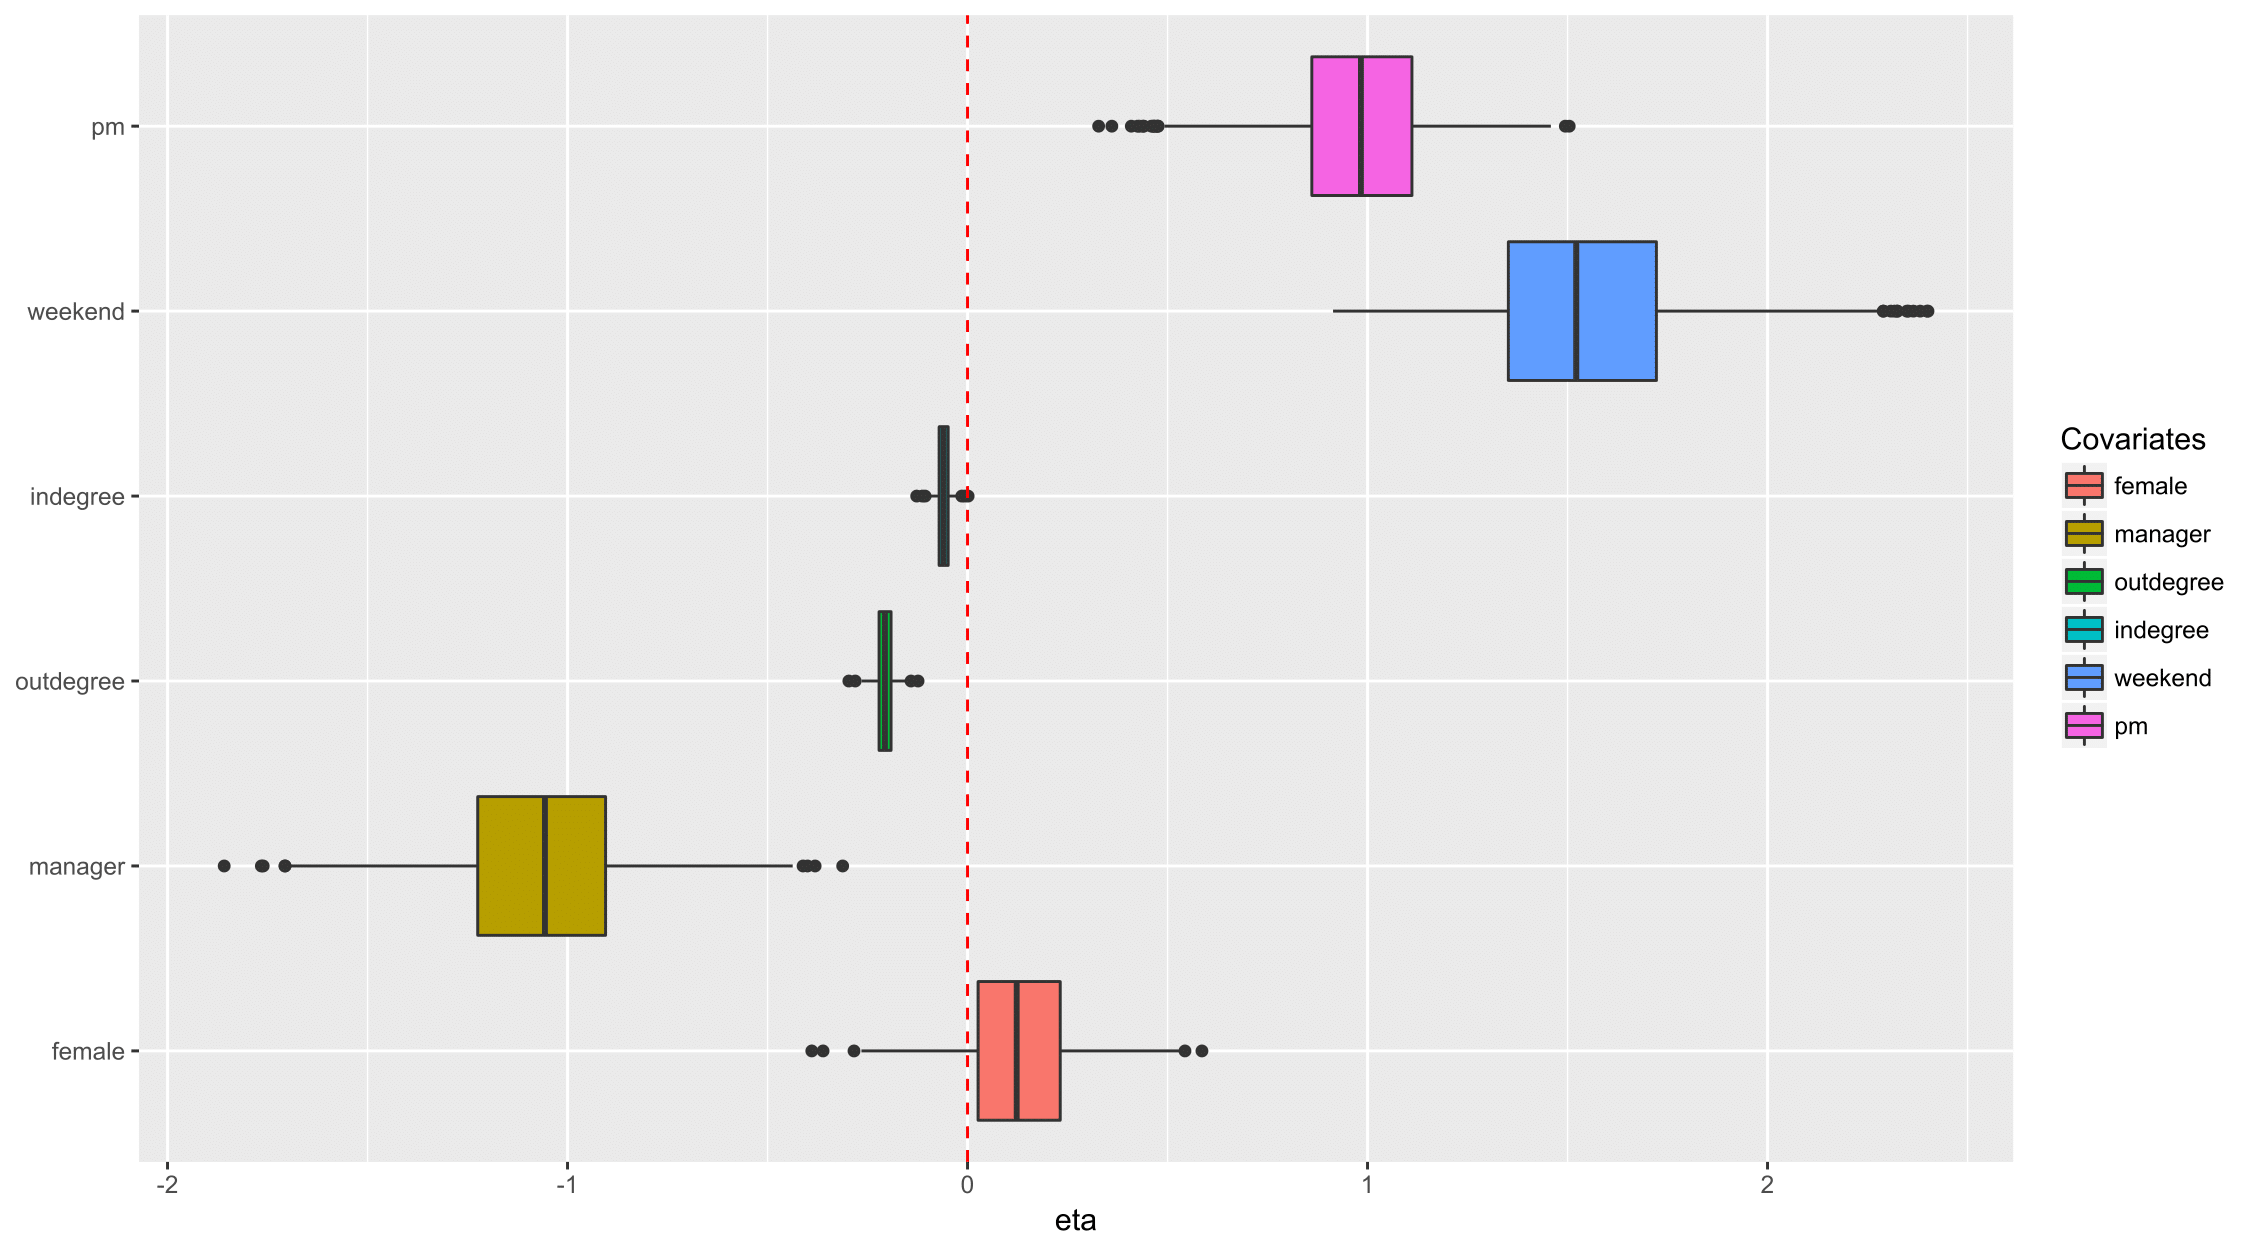
\includegraphics[width=0.89\textwidth]{img/etaest-1.png}	
				\caption {Posterior distribution of $\boldsymbol{\eta}$ estimates.}
				\label{figure:etaresults}
			\end{figure}
	\begin{equation*}
	\begin{aligned}
	&\log(\tau_{ad}) \sim N(\mu_{ad}, \sigma_\tau^2), \mbox{ with }\\
	&\mu_{ad} = \eta_{1}+\eta_{2} y_{ad2}\ldots+\eta_{7}y_{ad7}.
	\end{aligned}
	\end{equation*}
	To begin with, the posterior estimates of two temporal effects---``weekend" and 		AM/PM"---indicate that if the ${(d-1)}^{th}$ email was sent during the weekend or after midday, then the time to $d^{th}$ email is expected to take $\exp(1.552)\approx 4.722$ hours and $\exp(0.980)\approx2.665$ hours longer, respectively, compared to their counterparts (i.e., weekdays and am). On the contrary, the covariates ``manager", ``outdegree", and ``indegree" turn out to shorten the amount of time to next email. For example, being a county manager (i.e., the manager of department managers) lowers the expected value of $\log(\tau_{ad})$ by $\hat{\eta}_3 = -1.070$, since the manager in general sends or receives a lot more emails which may shorten the response time and many of those emails. This argument is also supported by the posterior estimates for ``outdegree" and ``indegree" statistics, where the estimated coefficients are approximately $\hat{\eta}_4=-0.206$ and $\hat{\eta}_5=-0.060$, respectively. Gender of the department manager is shown to have no significant effect on time increments. In addition, the posterior mean estimates for variance parameter $\sigma^2_\tau$ in lognormal distribution is approximately $\hat{\sigma}^2_\tau=14.093$ with its 95\% credible interval $(12.709, 15.555)$, indicating that there exists huge variability in the time increments of emails.
	
\section{Conclusion}\label{sec:conclusion}
Motivated by the relational event model \citep{Butts2008} and its variants for time-stamped networks, the hyperedge event model (HEM) can effectively learn the underlying edge generating and timestamp generating structures of event data, while allowing flexibity in the covariate specifications and the distributional assumption of time increments.
Accounting for the hyperedges, we make better use of events with hyperedges than modeling them as duplicate edges. In modeling the timestamps of the events, our generalized linear model (GLM) based formulation eliminates the need to stick with one distribution (e.g., exponential distribution), and we also provide an algorithm for predictive experiment that helps to learn which distribution better fits the data. To sum, the HEM's flexible generative process thus leads to more accurate and precise inference on model parameters.

We have demonstrated effectiveness of our model by analyzing Montgomery County government emails, which includes numerous hyperedges. The estimated covariate effects reveal that the HEM is able to understand the structural dynamics similar to those used in the exponential random graph model (ERGM), while the model additionally allows separate covariates and the corresponding parameters for generative processes of edges and timestamps. Although we illustrate the entire framework and application in the context
of one type of hyperedges, a single sender and multiple receivers, our model can be easily extended to allow the opposite case, a single receiver and multiple senders, by slight modification of the generative process. This extension involves promissing applications including international sanctions and co-sponsorship of bills. Furthermore, while currently the model's applicability is limited to small-sized networks since we assume fixed set of nodes across entire timepoints, we can adjust the model to allow time-varying nodes or improve its computational efficiency such that the model is well applicable to large-scale networks. Considering the recent explosion of network dataset with huge number of nodes (e.g., online comnunications), the development of model adjustments for better applicability are objects of future work.

\begin{acknowledgement}
	This work was supported in part by the University of Massachusetts Amherst Center for Intelligent Information Retrieval and in part by National Science Foundation grants DGE-1144860, SES-1619644, and CISE-1320219. Any opinions, findings, and conclusions or recommendations are those of the authors and do not necessarily reflect those of the
	sponsors.
\end{acknowledgement}

\section*{Appendix}
	\subsection*{Appendix A: Alternative Generative Process} \label{appendix:alternativeGP}
		\begin{algorithm}[H]
			\SetAlgoLined
			\caption{Generative Process: one receiver and one or more senders}
			\begin{algorithmic}
			\STATE \textbf{Input}: number of edges and nodes $(D, A)$, covariates $(\boldsymbol{x}, \boldsymbol{y})$, and the coefficients $(\boldsymbol{b}, \boldsymbol{\eta})$
							\vskip 0.1in				
				\FOR{d=1 to D}
				\FOR{r=1 to $A$}
				\FOR{a=1 to $A$ (a $\neq$ r)}
				\STATE	set $\lambda_{adr} = {\boldsymbol{b}}^{\top}\boldsymbol{x}_{adr}$
				\ENDFOR
				\STATE	draw $\boldsymbol{u}_{rd}  \sim
				\mbox{MB}_G(\boldsymbol{\lambda}_{rd})$
				\STATE		set $\mu_{rd} = g^{-1}(\boldsymbol{\eta}^\top \boldsymbol{y}_{rd})$
				\STATE		draw $\tau_{rd} \sim f_\tau(\mu_{rd}, \sigma_\tau^2)$
				\ENDFOR
				\IF {$n \geq 2$ tied events} 
				\STATE	set ${r}_d=\mbox{argmin}_{r}(\tau_{rd})$
				\STATE	set $\boldsymbol{a}_d=\boldsymbol{u}_{r_d d},\ldots,\boldsymbol{a}_{d+n-1}= ,\boldsymbol{u}_{r_{d+n-1} d}$
				\STATE	set $t_d, \ldots, t_{d+n-1}=t_{d-1} + \min_r\tau_{rd}$
				\STATE		jump to $d = d+n$
				\ELSE
				\STATE	set ${r}_d = \mbox{argmin}_{r}(\tau_{rd}) $
				\STATE	set $\boldsymbol{a}_d= \boldsymbol{u}_{r_d d}$
				\STATE	set $t_d =t_{d-1} + \min_r\tau_{rd}$
				\ENDIF
				\ENDFOR
			\end{algorithmic}
			\label{alg:generative2}
		\end{algorithm}
	\subsection*{Appendix B: Normalizing Constant of MB$_{G}$}\label{appendix: non-empty Gibbs measure}
	Our probability measure ``MB$_{G}$''---the multivariate Bernoulli distribution with non-empty Gibbs measure---defines the probability of sender $a$ selecting the binary receiver vector $\boldsymbol{u}_{ad}$ as
	\begin{equation*} 
	\begin{aligned}
	& \Pr(\boldsymbol{u}_{ad}|\boldsymbol{b}, \boldsymbol{x}_{ad}) = \frac{1}{Z(\boldsymbol{\lambda}_{ad})}\exp\Big(\mbox{log}\big(\text{I}(\lVert \boldsymbol{u}_{ad} \rVert_1 > 0)\big) + \sum_{r \neq a} \lambda_{adr}u_{adr} \Big),
	\end{aligned}
	\end{equation*}
	where the receiver intensity is a linear combination of edge covariates---i.e., $\lambda_{adr} = {\boldsymbol{b}}^{\top}\boldsymbol{x}_{adr}$---as defined in Secton \ref{subsec: Tie}.
	
	To use this distribution efficiently, we derive a closed-form expression for $Z(\boldsymbol{\lambda}_{ad})$ that does not require brute-force summation over the support of $\boldsymbol{u}_{ad}$ (\textit{i.e.} $\forall \boldsymbol{u}_{ad} \in [0,1]^A$). We recognize that if $\boldsymbol{u}_{ad}$ were drawn via independent Bernoulli distributions in which $\Pr({u}_{adr}=1|\boldsymbol{b}, \boldsymbol{x}_{ad})$ was given by logit$(\lambda_{adr})$, then 
	\begin{equation*}
	\Pr(\boldsymbol{u}_{ad}|\boldsymbol{b}, \boldsymbol{x}_{ad}) \propto \exp\Big(\sum_{r \neq a } \lambda_{adr}u_{adr}\Big).  	 
	\end{equation*}
	This is straightforward to verify by looking at 
	\begin{equation*}
	\begin{aligned}
	&\Pr(u_{adr}=1|\boldsymbol{u}_{ad[-r]}, \boldsymbol{b}, \boldsymbol{x}_{ad})
	=\frac{\exp{(\lambda_{adr})}}{\exp{(\lambda_{adr})} + 1}.
	\end{aligned}\end{equation*}
	We denote the logistic-Bernoulli normalizing constant as $Z^{l}(\boldsymbol{\lambda}_{ad})$, which is defined as 
	\begin{equation*}
	Z^{l}( \boldsymbol{\lambda}_{ad})=\sum_{\boldsymbol{u}_{ad} \in [0,1]^{A}} \exp\Big(\sum_{r\neq a} \lambda_{adr}u_{adr}\Big).
	\end{equation*}
	Now, since 
	\begin{equation*}
	\begin{aligned}
	&\exp\Big(\mbox{log}\Big(\text{I}(\lVert \boldsymbol{u}_{ad} \rVert_1 > 0)\Big) + \sum_{r \neq a} \lambda_{adr}u_{adr} \Big)= \exp\Big( \sum_{r \neq a} \lambda_{adr}u_{adr} \Big),
	\end{aligned}
	\end{equation*}
	except when $\lVert \boldsymbol{u}_{ad} \rVert_1=0$, we note that 
	\begin{equation*}
	\begin{aligned}
	Z(\boldsymbol{\lambda}_{ad})& = Z^{l}(\boldsymbol{\lambda}_{ad}) -\exp\Big( \sum\limits_{\forall u_{adr}=0}\lambda_{adr}u_{adr} \Big)
	\\& = Z^{l}(\boldsymbol{\lambda}_{ad}) -  1.
	\end{aligned}
	\end{equation*}
	We can therefore derive a closed form expression for $Z(\boldsymbol{\lambda}_{ad})$ via a closed form expression for $Z^{l}(\boldsymbol{\lambda}_{ad})$. This can be done by looking at the probability of the zero vector under the logistic-Bernoulli model:
	\begin{equation*}
	\begin{aligned}
	&\frac{1}{Z^{l}(\boldsymbol{\lambda}_{ad})}\exp\Big(\sum\limits_{\forall u_{adr}=0}\lambda_{adr}u_{adr} \Big)= \prod_{r \neq a}   \Big(1-\frac{ \exp{(\lambda_{adr})}}{\exp{(\lambda_{adr})} + 1}\Big).
	\end{aligned}  
	\end{equation*}
	Then, we have 
	\begin{equation*}
	\begin{aligned}
	& \frac{1}{Z^{l}(\boldsymbol{\lambda}_{ad})} &= \prod\limits_{r \neq a}\frac{1}{ \exp(\lambda_{adr})+ 1}.
	\end{aligned}  
	\end{equation*}
	Finally, the closed form expression for the normalizing constant is  
	\begin{equation*}
	\begin{aligned}Z(\boldsymbol{\lambda}_{ad}) = \prod_{r \neq a } \big(\mbox{exp}(\lambda_{adr}) + 1\big)-1.
	\end{aligned}  
	\end{equation*}
\newpage
	\subsection*{Appendix C: Comparison of PPC Results: log-normal vs. exponential}\label{appendix: PPCexp}
		\begin{figure}[H]
			\centering
			\begin{tabular}[t]{cc}
				\begin{subfigure}[b]{0.495\textwidth}
					\caption{Outdegree distribution}
					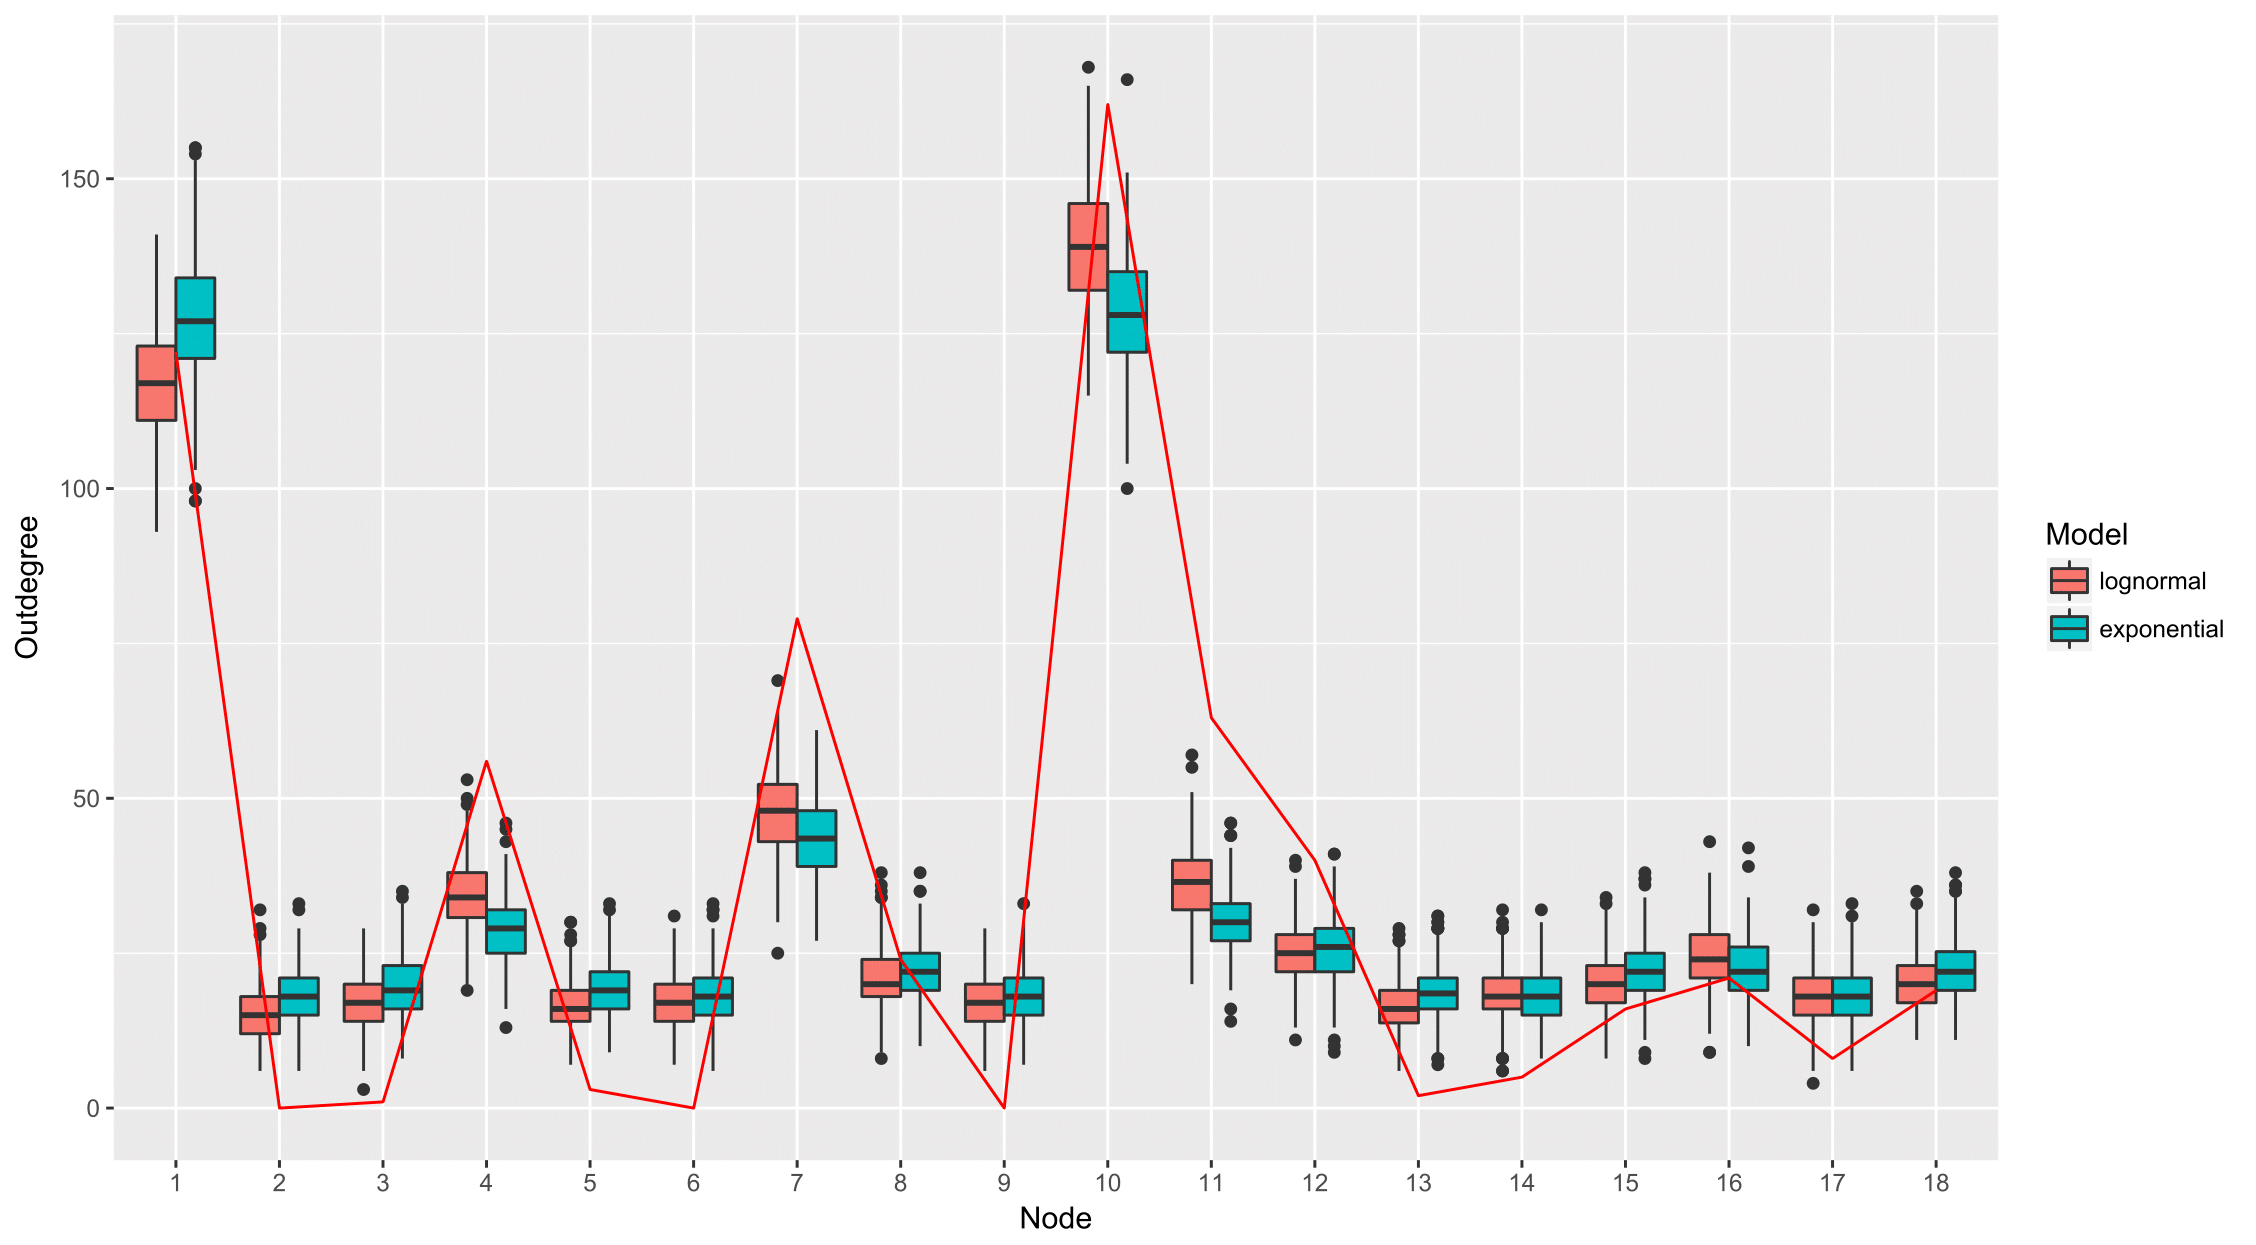
\includegraphics[width=\textwidth]{img/outdegree_two-1.png}	
				\end{subfigure}
				\begin{subfigure}[b]{0.495\textwidth}
					\caption{Indegree distribution}
					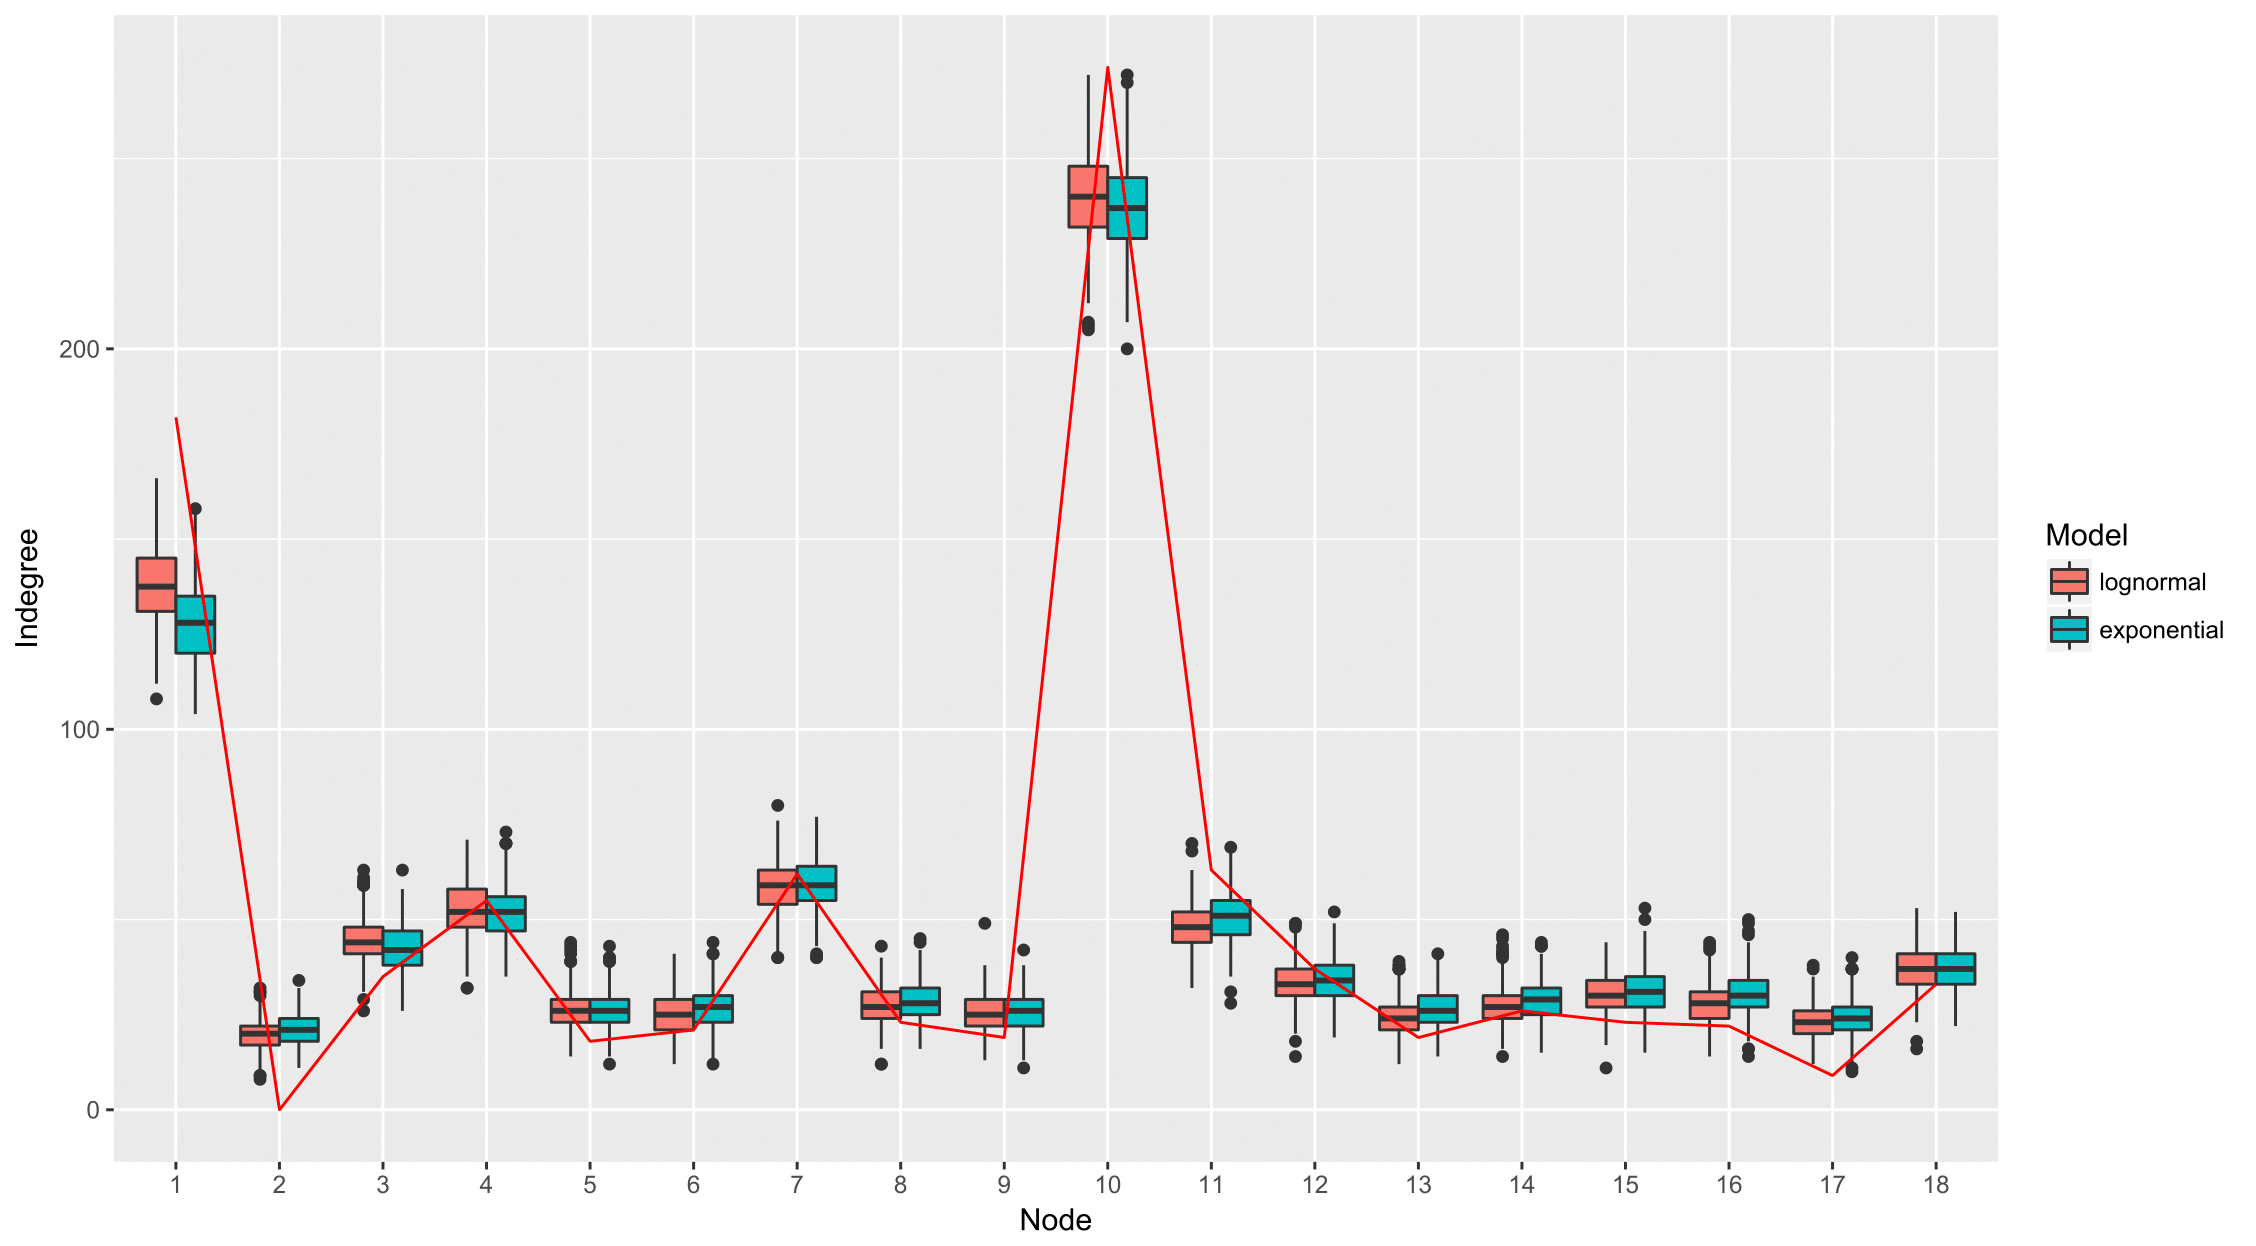
\includegraphics[width=\textwidth]{img/indegree_two-1.png}	
				\end{subfigure}\\
				\begin{subfigure}[b]{0.495\textwidth}
					\caption{Receiver size distribution}
					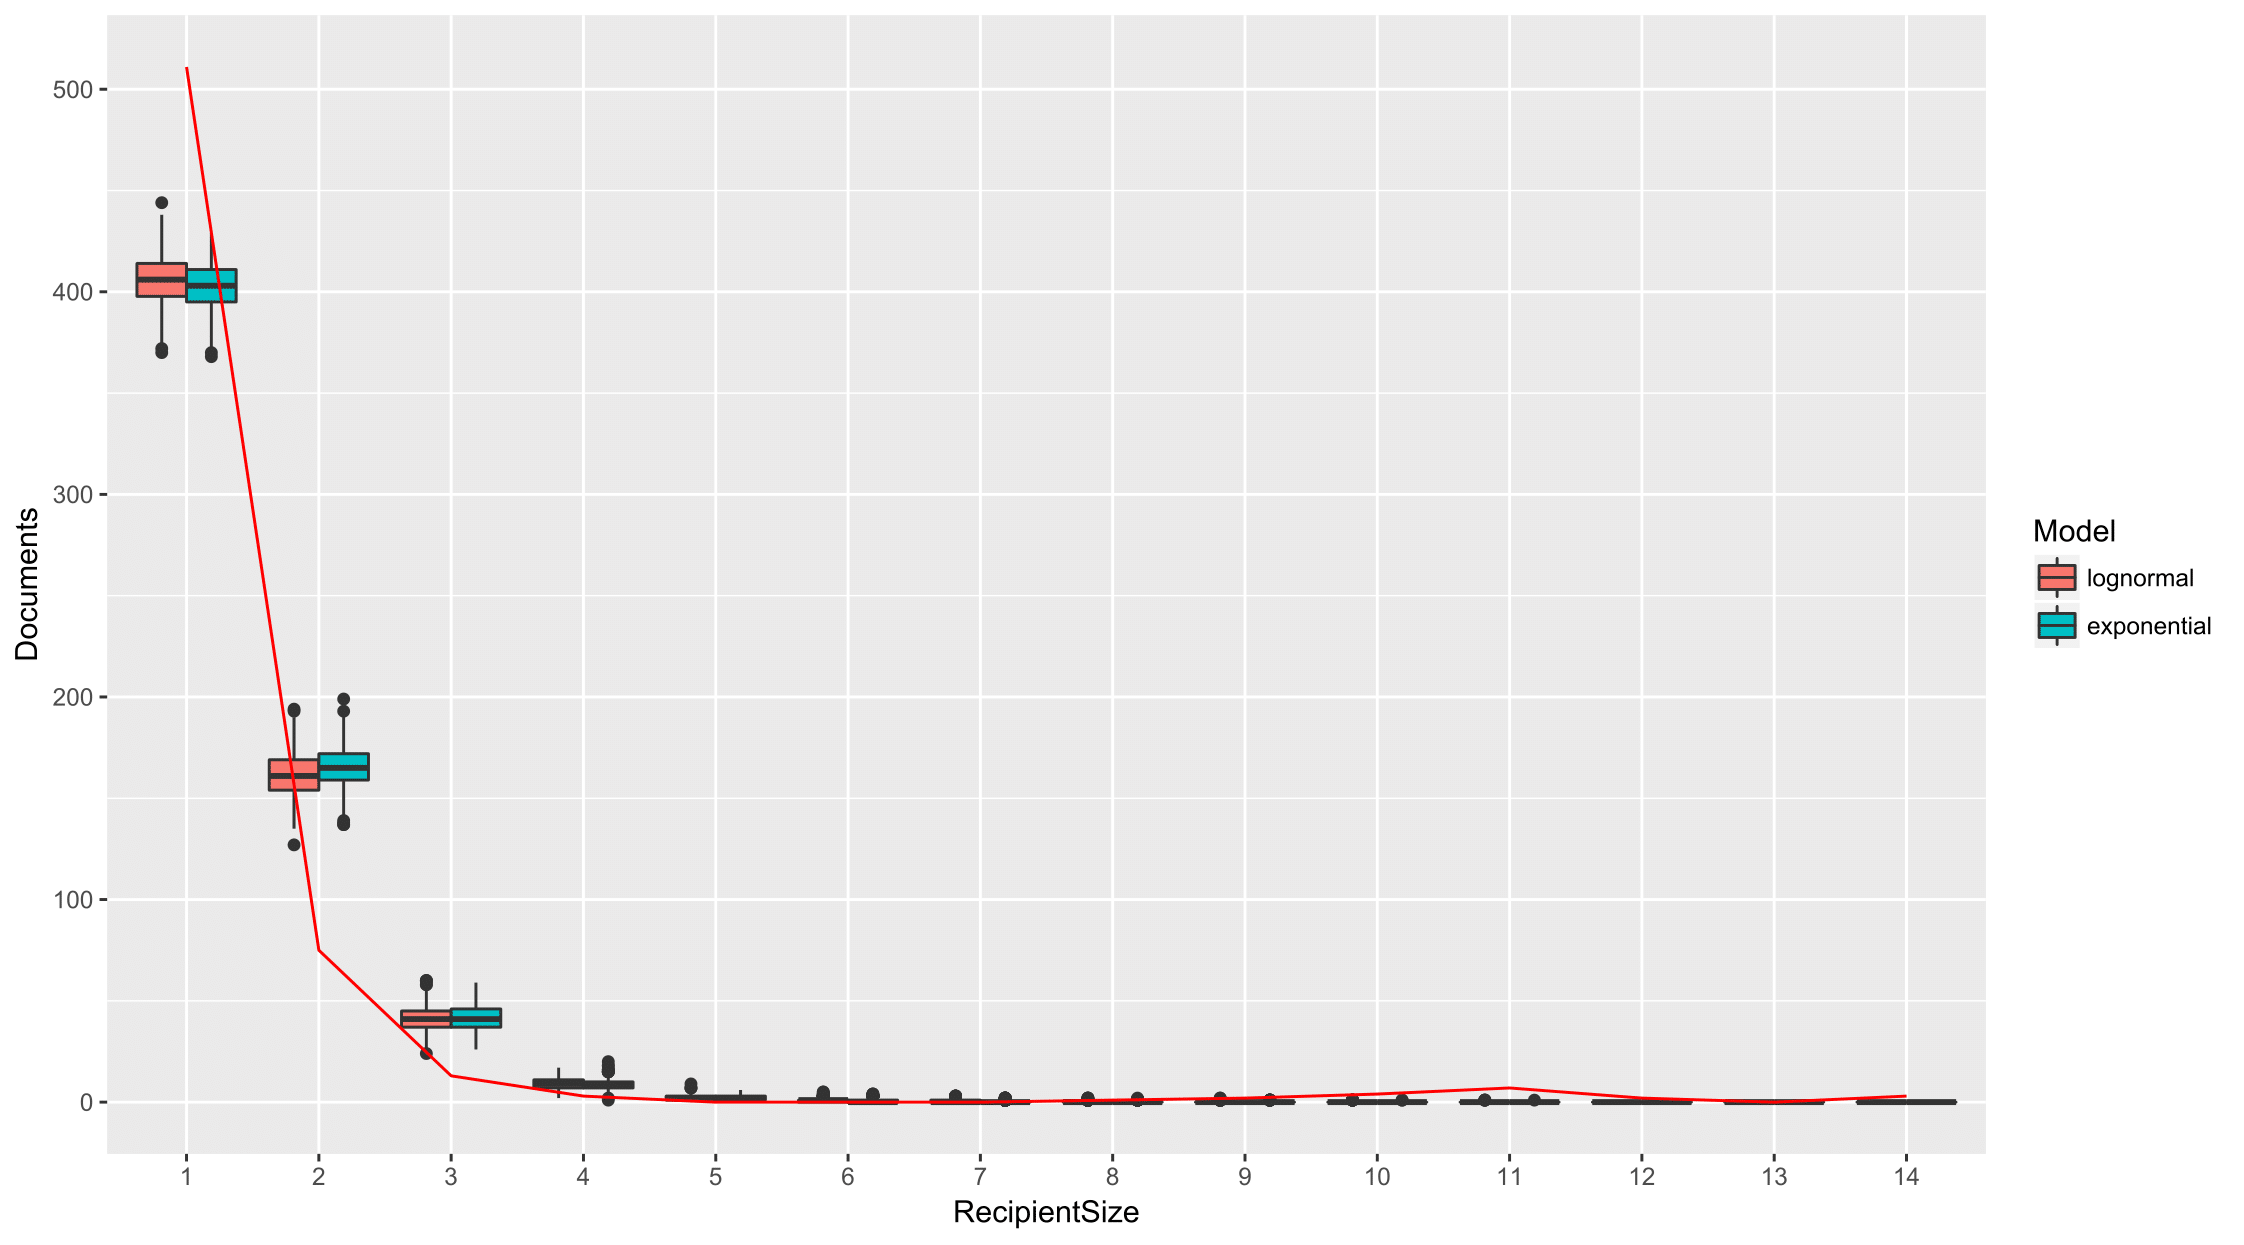
\includegraphics[width=\textwidth]{img/recipientsize_two-1.png}	
				\end{subfigure}
				\begin{subfigure}[b]{0.495\textwidth}
					\centering
					\caption{PPplot for time increments}
					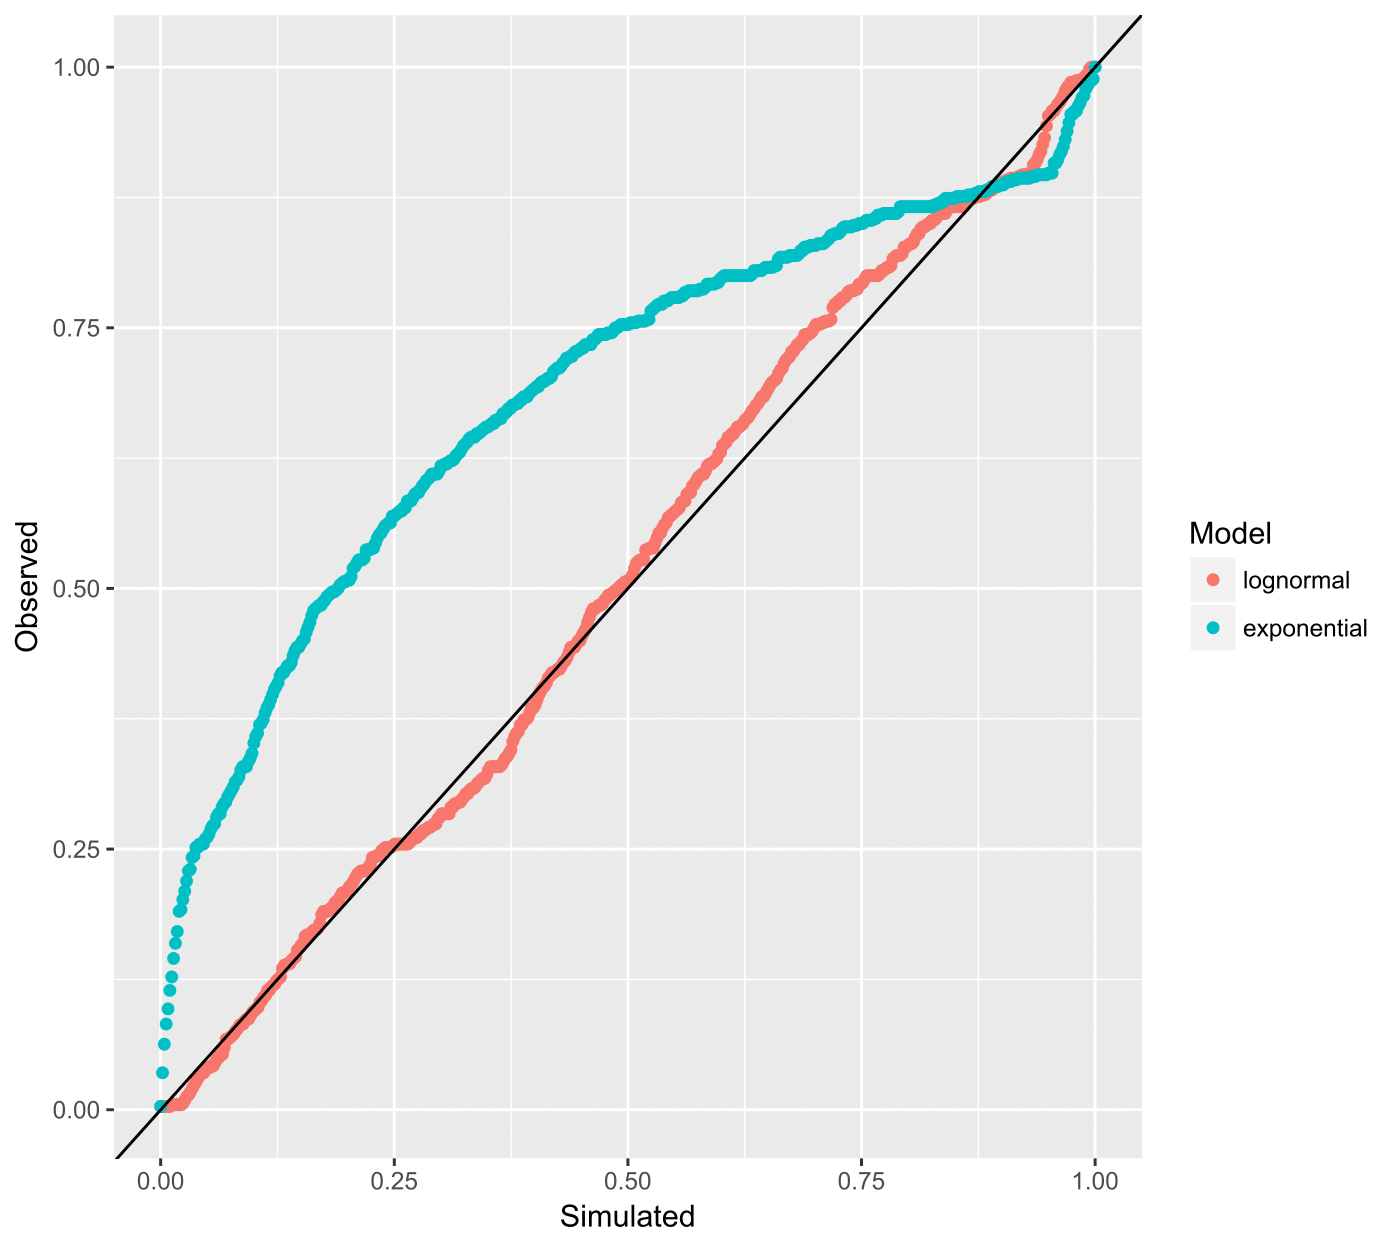
\includegraphics[width=0.625\textwidth]{img/timepp_two-1.png}
				\end{subfigure}
			\end{tabular}
			\caption {Comparison of PPC results between log-normal (\textit{red}) and exponential (\textit{green}) distributions. Blue lines denote the observed statistics in (a)--(c) and denotes the diagonal line in (d).}
			\label{figure:PPCtwo}
		\end{figure}
		\newpage
	\subsection*{Appendix D: Convergence Diagnostics}\label{appendix: convergence}
		\begin{figure}[H]
			\centering
			\begin{tabular}[t]{cc}
				\begin{subfigure}[b]{0.495\textwidth}
					\caption{Traceplots of $\boldsymbol{b}$}
					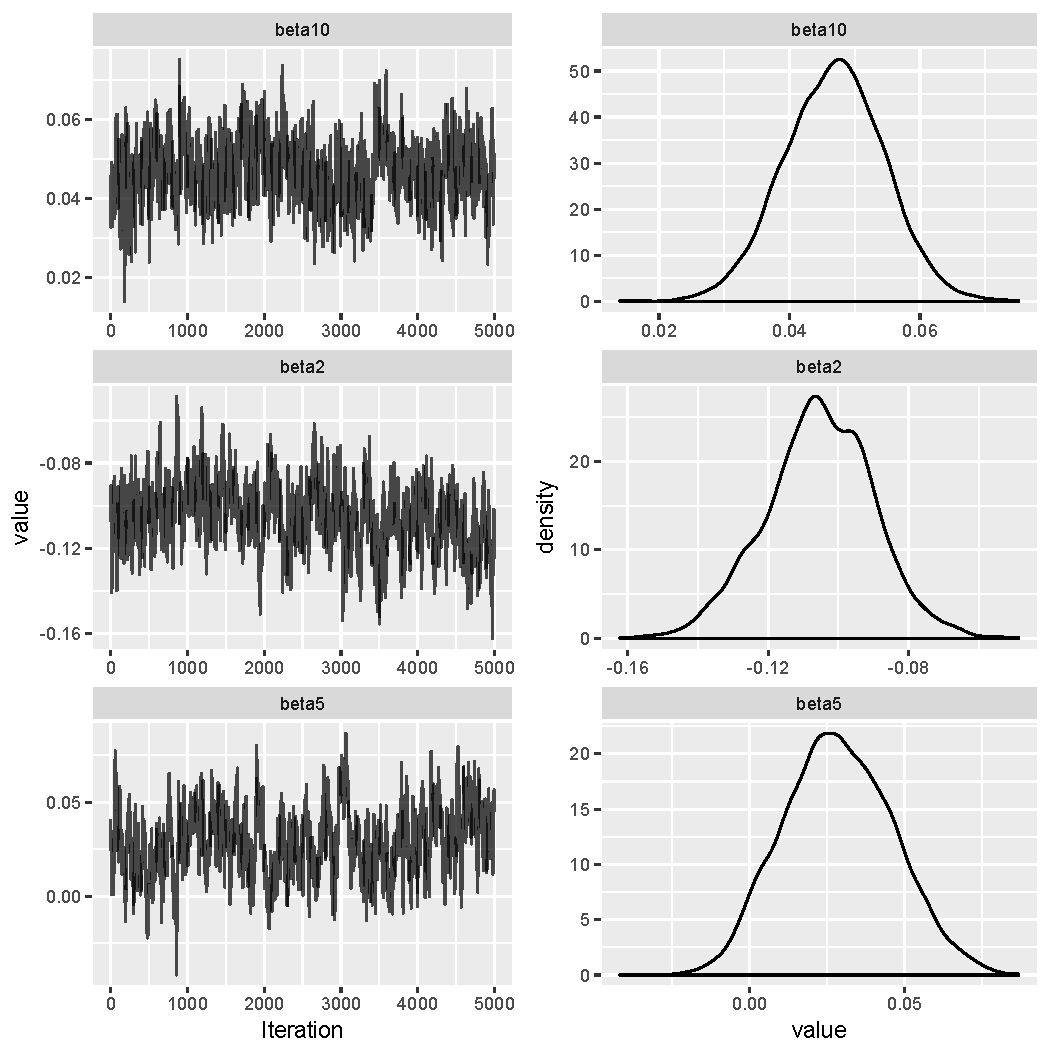
\includegraphics[width=\textwidth]{img/betatrace.pdf}	
				\end{subfigure}
				\begin{subfigure}[b]{0.495\textwidth}
					\caption{Traceplot of $\boldsymbol{\eta}$}
					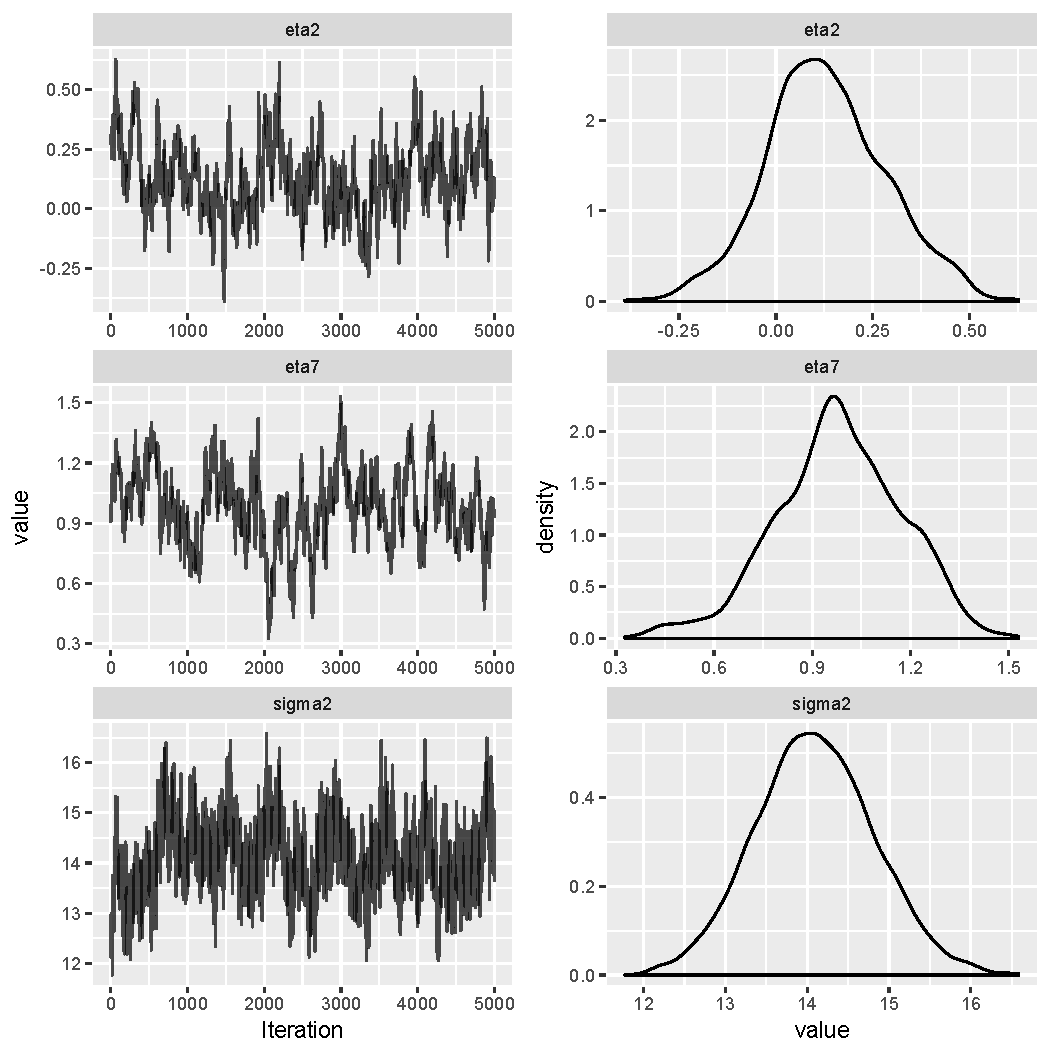
\includegraphics[width=\textwidth]{img/etatrace.pdf}	
				\end{subfigure}\\
				\begin{subfigure}[b]{0.495\textwidth}
					\caption{Geweke diagnostics for $\boldsymbol{b}$}
					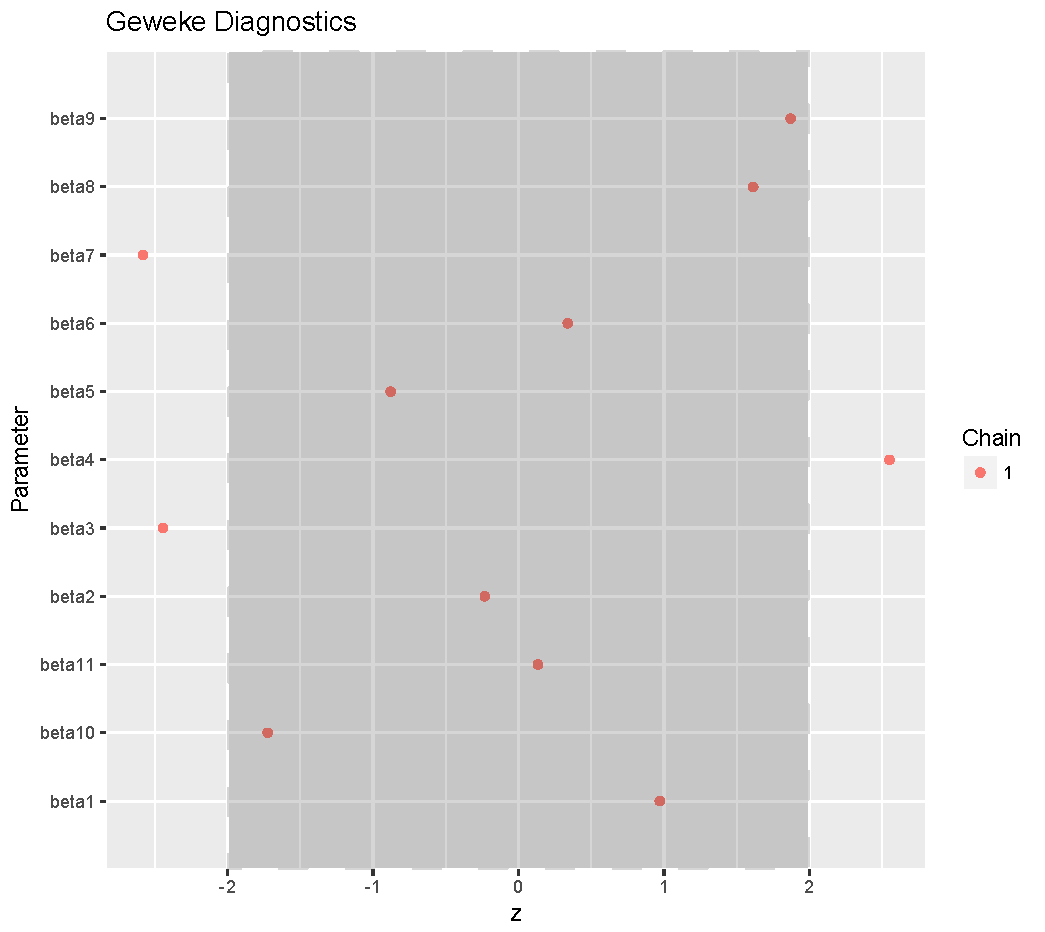
\includegraphics[width=\textwidth]{img/betageweke.pdf}	
				\end{subfigure}
				\begin{subfigure}[b]{0.495\textwidth}
					\centering
					\caption{Geweke diagnostics for $\boldsymbol{\eta}$ and $\sigma^2_\tau$}
					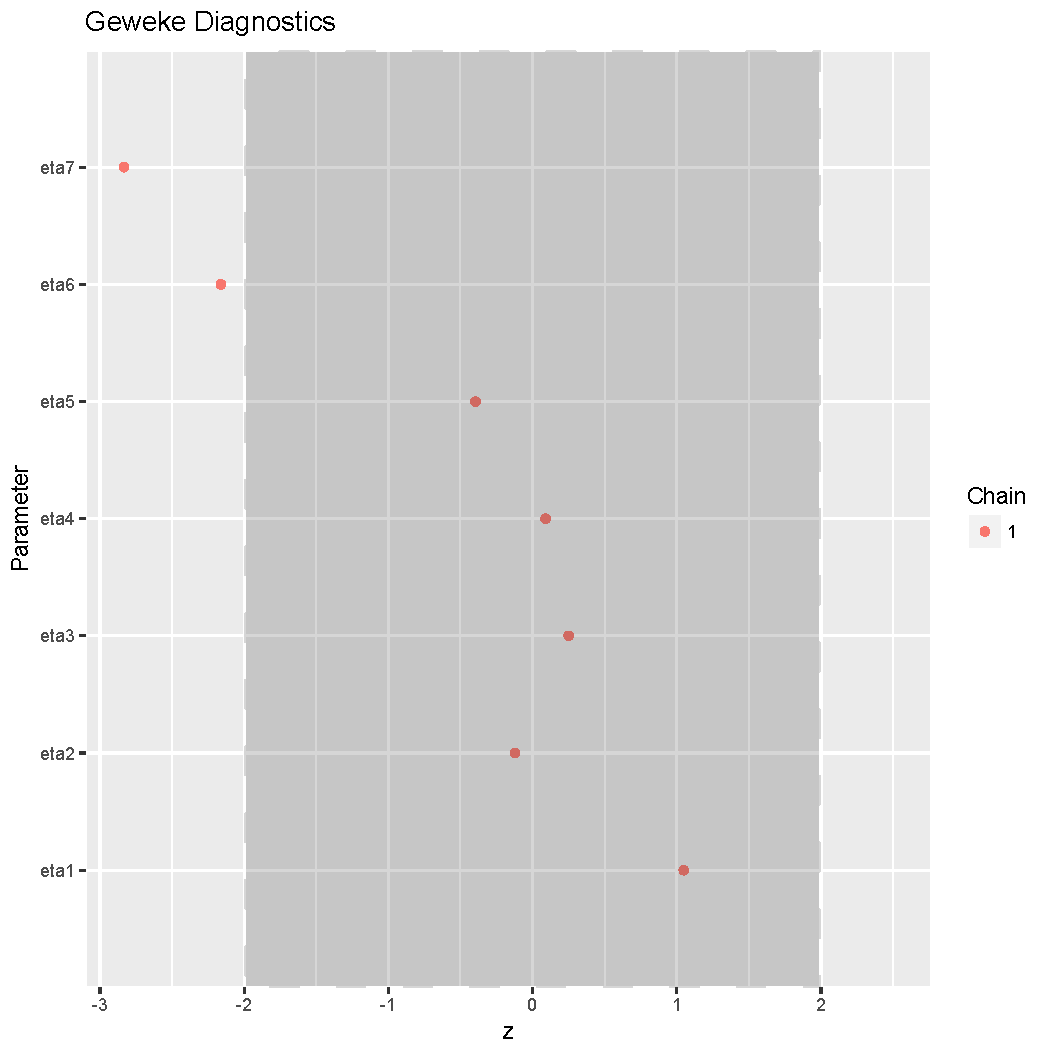
\includegraphics[width=0.89\textwidth]{img/etageweke.pdf}
				\end{subfigure}
			\end{tabular}
			\caption {Convergence diagnostics from log-normal distribution.}
			\label{figure:convergencediag}
		\end{figure}
	\begin{supplement}
\sname{Supplement A}\label{suppA} 
\stitle{Title of the Supplement A}
\slink[url]{http://www.some-url-address.org/dowload/0000.zip}
\sdescription{Add description for supplement material.}
\end{supplement}


\bibliographystyle{ba}
\bibliography{baHEM}




\end{document}

